\documentclass[11pt,a4paper]{article}

% ---- Packages ----
\usepackage[utf8]{inputenc}
\usepackage[T1]{fontenc}
\usepackage{mathpazo}           % Palatino font (matches MDPI)
\usepackage{amsmath,amssymb}
\usepackage{graphicx}
\usepackage{booktabs}
\usepackage{longtable}
\usepackage{tabularx}
\usepackage{float}
\usepackage{geometry}
\usepackage{setspace}
\usepackage[hidelinks]{hyperref}
\usepackage{cleveref}
\usepackage{caption}
\usepackage{pdflscape}          % landscape pages for wide tables

% ---- Page layout ----
\geometry{margin=2.5cm}
\onehalfspacing
\setlength{\parindent}{0pt}
\setlength{\parskip}{6pt plus 2pt minus 1pt}

% ---- Font sizes ----
% Smaller captions for figures and tables
\captionsetup{font=small, labelfont=bf}
% Equation numbers on the right (default in article class)

% ---- Pandoc compat ----
\providecommand{\tightlist}{\setlength{\itemsep}{0pt}\setlength{\parskip}{0pt}}

% ---- Line numbers for review ----
\usepackage{lineno}
\linenumbers

% ---- Section font sizes (scaled for 11pt body) ----
\usepackage{titlesec}
\titleformat{\section}{\large\bfseries}{\thesection}{1em}{}
\titleformat{\subsection}{\normalsize\bfseries}{\thesubsection}{1em}{}
\titleformat{\subsubsection}{\normalsize\itshape}{\thesubsubsection}{1em}{}
\titleformat{\paragraph}[runin]{\normalsize\bfseries}{\theparagraph}{1em}{}[.]

% ============================================================
\title{\Large A Scalable Framework for Enhancing Satellite-Derived Daily Precipitation: Adjusting Values, Aligning Distributions, and Preserving Extremes}


\author{\normalsize
Benny Istanto\textsuperscript{1,*} \and
Rizaldi Boer\textsuperscript{2,3} \and
I Putu Santikayasa\textsuperscript{2,4}
}

\date{\small
\textsuperscript{1} Applied Climatology Study Program, Department of Geophysics and Meteorology,\\
Bogor Agricultural University, Bogor 16680, Indonesia\\[2pt]
\textsuperscript{2} Department of Geophysics and Meteorology, Bogor Agricultural University, Bogor 16680, Indonesia\\[2pt]
\textsuperscript{3} International Research Institute for Environment and Climate Change,\\
Bogor Agricultural University, Bogor 16680, Indonesia\\[2pt]
\textsuperscript{4} Center for Climate Risk and Opportunity Management in South East Asia and Pacific,\\
Bogor Agricultural University, Bogor 16680, Indonesia\\[6pt]
* Correspondence: bennyistanto@gmail.com
}

\begin{document}
\maketitle

\begin{abstract}
Accurate daily precipitation estimates are essential for hydrological modeling, climate risk assessment, and disaster preparedness. Satellite-based precipitation products such as the Integrated Multi-satellitE Retrievals for Global Precipitation Measurement (IMERG) provide global coverage but exhibit systematic biases in daily accumulations, particularly in representing extreme precipitation events. This study presents a hybrid bias correction framework (LSEQM+DL) for daily satellite precipitation that sequentially integrates Linear Scaling (LS) for mean bias removal, Empirical Quantile Mapping (EQM) with Generalized Pareto Distribution (GPD) tail adjustment for distributional alignment, and a Convolutional Neural Network (CNN) refinement that selectively targets extreme precipitation pixels. A station density confidence mask modulates the deep learning influence based on gauge network density, so that the CNN refinement is strongest where the reference dataset (CPC Unified Gauge-Based Analysis of Daily Precipitation, CPC-UNI) is best constrained by observations. Applied to daily IMERG Late Run precipitation over Indonesia (2001--2025) and evaluated against CPC-UNI and 171 independent station observations from Indonesia's Meteorological, Climatological, and Geophysical Agency (BMKG), the framework is assessed through three evaluation pillars aligned with its design objectives: adjusting values, aligning distributions, and preserving extremes. At independent BMKG station locations, the hybrid correction brings the standard deviation ratio from 0.71 (LS) to 1.00 (LSEQM+DL, toward unity), the relative bias from $-$11.4\% to $-$0.6\%, and the 99th-percentile ratio from 0.71 to 1.01, indicating convergence of the corrected distribution toward the observed precipitation statistics. The wet-day frequency ratio improves from 1.21 (LS) to 0.95 (LSEQM+DL), reducing a 21\% overestimation of wet-day occurrence to within 5\% of observed. These improvements come at a known cost: event detection (POD) decreases from 0.78 to 0.65, reflecting the trade-off inherent to distributional correction methods that adjust marginal statistics without modifying temporal sequencing. Pixel-level temporal accuracy metrics (correlation, root mean square error, Nash-Sutcliffe efficiency) remain largely unchanged, confirming that the framework improves statistical properties rather than day-to-day prediction skill. The World Meteorological Organization (WMO) multi-threshold verification at station locations shows maintained detection skill at rainfall thresholds up to 100 mm/day. Because the approach relies on globally available satellite and gauge-analysis datasets, it is applicable to other tropical and subtropical regions with sparse gauge networks, though recalibration of CNN hyperparameters and GPD thresholds may be required for different climate regimes.

\noindent\textbf{Keywords:} Bias Correction, Satellite Precipitation, IMERG, Daily Precipitation, Extreme Events, Deep Learning, Quantile Mapping, Generalized Pareto Distribution, Quality Assessment, Indonesia
\end{abstract}

\newpage


\section{Introduction}\label{introduction}

Accurate and timely precipitation estimates are critical for a wide
range of scientific and societal applications, including flood
forecasting, drought monitoring, hydrological modeling, and climate risk
assessments. Satellite-derived precipitation products, such as those
from the Global Precipitation Measurement (GPM) mission \cite{ref1,ref2}, have
greatly expanded the global coverage of precipitation observations,
especially over regions with sparse ground station networks. However,
despite their transformative role, satellite-based estimates often
suffer from systematic biases, spatial inconsistencies, and challenges
in capturing the full spectrum of precipitation variability \cite{ref3},
particularly for extreme rainfall events. These limitations reduce the
reliability of satellite data for operational and scientific
applications that depend on an accurate depiction of both mean
conditions and high-impact extremes.

A wide range of bias correction techniques has been developed to address
these challenges. Traditional statistical methods, such as Linear
Scaling (LS), effectively correct mean biases by adjusting the overall
magnitude of satellite estimates to align with ground-based observations
\cite{ref4}. Empirical Quantile Mapping (EQM) extends this correction by
aligning the entire distribution of satellite precipitation with the
reference distribution, adjusting not only the mean but also
higher-order statistical moments \cite{ref5,ref6}. More recently, methods such
as Generalized Pareto Distribution (GPD) fitting have been introduced to
specifically address biases in the tails of precipitation distributions,
aiming to better preserve extreme events \cite{ref7}. In parallel, advances
in machine learning (ML) and deep learning (DL) have opened new
possibilities for bias correction, enabling more flexible and nonlinear
mappings between satellite and reference data \cite{ref8}. Convolutional
Neural Networks (CNNs) provide powerful capabilities for modeling
complex spatial patterns that traditional statistical methods may
overlook \cite{ref9,ref10}.

Despite these advances, several critical gaps remain. Traditional bias
correction techniques, while effective in adjusting mean and moderate
rainfall distributions, often underperform in preserving the frequency
and magnitude of extreme precipitation events \cite{ref8,ref11}, precisely the
events most relevant for disaster risk management and climate
adaptation. Furthermore, many machine learning approaches lack
integration with physically interpretable statistical corrections, which
can lead to potential issues such as overfitting, instability, or a lack
of transparency \cite{ref12}. There remains a need for a hybrid approach
that simultaneously addresses mean biases, distributional alignment, and
extreme event preservation in a scalable and reproducible manner.

In this study, we propose a hybrid bias correction framework that
sequentially integrates Linear Scaling, Empirical Quantile Mapping with
gamma-based distribution fitting and GPD tail adjustment, and a Deep
Learning refinement step using Convolutional Neural Networks. The
framework is designed to improve daily satellite precipitation estimates
by systematically adjusting mean values, aligning distributions, and
preserving extremes. Using globally available datasets -- the Integrated
Multi-satellitE Retrievals for GPM (IMERG) Late Run (IMERG-L) satellite
precipitation \cite{ref2} and the CPC Global Unified Gauge-Based Analysis of
Daily Precipitation (CPC-UNI) gridded station observations \cite{ref13} --
the methodology is demonstrated over the Indonesian archipelago,
selected for its vulnerability to extreme rainfall and complex
topographic and climatic conditions. Correction quality is evaluated
through 31 verification metrics organized into a composite Continuous
Quality Index (CQI), providing a structured assessment across basic
statistical, distributional, and temporal dimensions \cite{ref14,ref15}.

To address the spatial heterogeneity inherent in gauge-based reference
datasets, the framework incorporates a station density confidence mask
that modulates the influence of the deep learning component based on
gauge network density. In regions where the CPC-UNI reference is
supported by dense station coverage, the CNN refinement is applied with
greater confidence. In station-sparse regions, where the reference
dataset relies on interpolation and may not accurately capture local
precipitation characteristics, the framework reverts toward purely
statistical corrections. This design provides a systematic approach for
managing reference dataset uncertainty in operational bias correction
over regions with heterogeneous observational networks.

\section{Conceptual Framework and Theoretical Background}

Improving satellite-derived precipitation estimates requires addressing
biases across multiple statistical dimensions: the mean, the
distributional structure, and the representation of extremes. Because
these biases are multi-dimensional, this study employs a hybrid
framework that sequentially integrates physical-statistical correction
methods with machine learning refinement, targeting improvements across
the entire precipitation spectrum.

\textbf{Rationale for a Hybrid Approach}

Single-method bias correction strategies often target specific aspects
of the precipitation distribution but leave other sources of error
unaddressed. Linear Scaling (LS) methods are effective at correcting
systematic mean biases but do not modify variance or higher-order
moments, leaving distributional mismatches largely unresolved
\cite{ref4,ref16}. Empirical Quantile Mapping (EQM) extends corrections to the
full distribution, aligning the cumulative distribution functions (CDFs)
between satellite and reference datasets \cite{ref5,ref6}. However, EQM may
underestimate or misrepresent the upper extremes, where observational
data sparsity and fitting uncertainty are most pronounced \cite{ref8}.

Extreme events, which are often underrepresented in station-based
datasets and distorted in satellite retrievals, require specialized
treatment. Generalized Pareto Distribution (GPD) fitting provides a
statistical mechanism to model precipitation behavior beyond high
thresholds, complementing EQM by refining the upper tail of the
distribution \cite{ref7}. Nevertheless, statistical methods alone may
struggle to capture complex spatial structures and local-scale anomalies
that influence extreme precipitation, particularly over heterogeneous
landscapes.

Recent advances in deep learning, particularly the application of
Convolutional Neural Networks (CNNs), offer a complementary tool for
bias correction. CNNs can learn nonlinear relationships between
satellite estimates and reference data, exploiting spatial correlations
and subtle patterns not easily captured by traditional techniques
\cite{ref9,ref17}. Integrating deep learning refinement after statistical
corrections allows the framework to adaptively correct localized errors
without undermining physical plausibility \cite{ref10}.

Thus, a sequential hybrid approach, starting with mean correction (LS),
progressing to distributional correction (EQM with GPD adjustment), and
culminating in spatially aware deep learning refinement, is proposed to
systematically address all facets of satellite precipitation bias. A
critical additional consideration is the spatial heterogeneity of
reference dataset quality: the CPC-UNI product, while globally
available, relies on interpolation in station-sparse regions and may not
accurately represent local extremes \cite{ref13,ref18}. The framework addresses
this through a station density confidence mask that modulates the deep
learning influence based on gauge availability, providing an explicit
mechanism for managing training target uncertainty.

The sequential structure of the proposed methodology is illustrated in
Figure 1.

\begin{figure}[H]
\centering
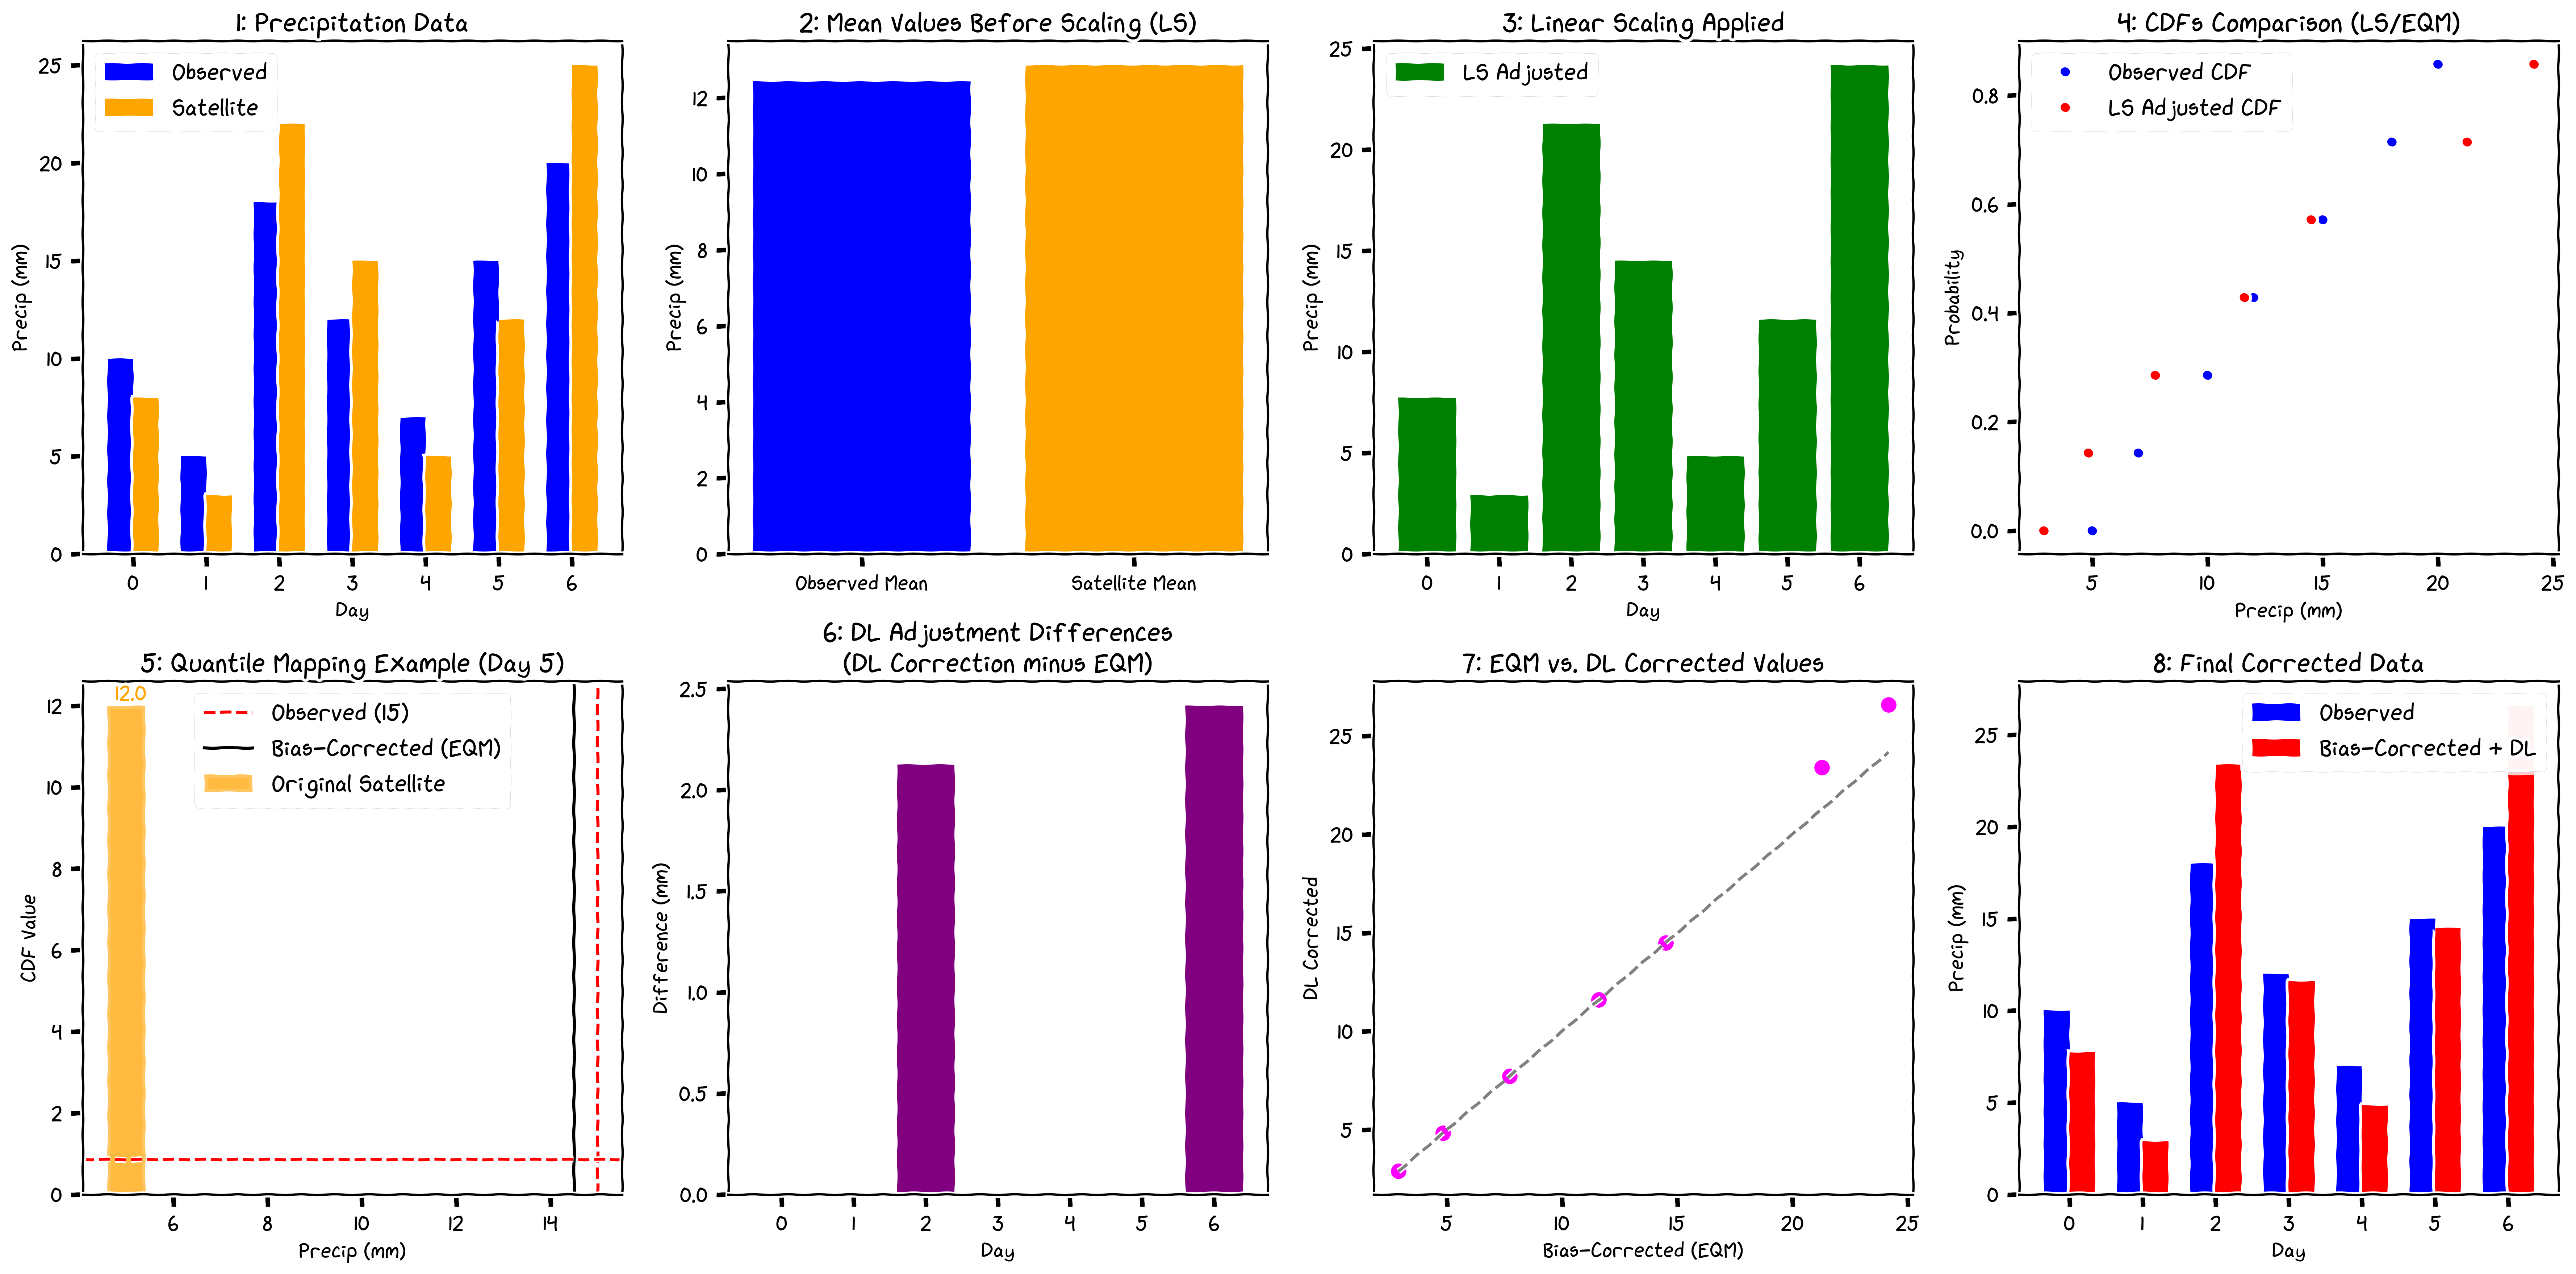
\includegraphics[width=\textwidth]{images/fig01_framework.png}
\caption{Conceptual workflow of the LSEQM+DL hybrid bias correction framework.\label{fig1}}
\end{figure}

The framework integrates sequential adjustments through LS for mean
correction, EQM with GPD tail adjustment for distributional alignment,
Deep Learning (DL) refinement targeting extreme precipitation
preservation, and station density confidence weighting to manage
reference dataset uncertainty.

\section{Methods}\label{methods}

Bias correction of satellite-derived precipitation products requires not
only robust methodological design but also careful data preparation and
study site selection. This chapter outlines the geographical focus of
the study, the datasets used, and the preprocessing steps taken to
ensure consistency and comparability between satellite and reference
observations. Each step is tailored to support the development of a
globally scalable bias correction framework that enhances precipitation
estimates across varying climatic and topographical conditions.

\subsection{Study Region}\label{study-region}

Indonesia, the world's largest archipelagic country, presents a complex
and challenging environment for precipitation estimation. Located
between the Indian and Pacific Oceans and straddling the equator,
Indonesia experiences a tropical climate characterized by high spatial
and temporal variability in rainfall \cite{ref19,ref20}. Topographical
diversity, ranging from lowland plains to mountainous regions exceeding
4,000 meters in elevation, further complicates precipitation patterns.
The country is highly vulnerable to extreme rainfall events that
frequently trigger flooding, landslides, and other hydrometeorological
disasters.

This study adopts Indonesia as the area of interest (AOI) due to its
critical need for improved precipitation monitoring and its
representative challenges for satellite-based hydrometeorological
applications. While the Indonesia's Meteorological, Climatological, and
Geophysical Agency (BMKG) station data used for validation are specific
to Indonesia, the primary datasets utilized for bias correction, IMERG
and CPC-UNI, are globally available. Moreover, the hybrid bias
correction methodology developed here is designed to be scalable and
replicable across other regions worldwide, supporting broader
applications in climate research, disaster risk reduction, and
hydrological modeling beyond Indonesia.

\subsection{Data and Preprocessing}\label{data-and-preprocessing}

Developing a reliable bias correction framework demands the careful
selection of datasets that represent both satellite-based estimates and
ground-based observations \cite{ref22}. This section describes the data
sources utilized and outlines the preprocessing steps undertaken to
harmonize their spatial and temporal characteristics.

\paragraph{IMERG Satellite Precipitation
Data}\label{imerg-satellite-precipitation-data}

The Integrated Multi-satellitE Retrievals for GPM (IMERG) Late Run
(IMERG-L) product is selected as the satellite-derived precipitation
dataset for this study \cite{ref2,ref21}. IMERG-L offers an optimal balance
between latency and data quality, providing near-real-time precipitation
estimates with a delay of approximately 14 hours. Unlike the IMERG Final
Run, which incorporates station data into its post-processing, the Late
Run product relies purely on satellite observations, making it ideal for
evaluating bias correction methods without the influence of gauge data
assimilation. IMERG-L data are available at a high spatial resolution of
0.1 degrees (\textasciitilde10 km) and are directly accessed from the
official NASA Goddard Earth Sciences Data and Information Services
Center (GES DISC).

\paragraph{IMERG Final Run for Complementary
Evaluation}

In addition to the IMERG-L data used for bias correction, this study
also utilizes the IMERG Final Run (IMERG-F) product as a complementary
evaluation dataset. IMERG-F incorporates gauge-based observations during
its post-processing, aiming to further improve precipitation accuracy
relative to purely satellite-derived estimates. Although it benefits
from station assimilation, the IMERG-F is not used in the bias
correction procedure itself to maintain independence between correction
inputs and validation references. Instead, the IMERG-F is employed for
comparative analysis, providing an additional benchmark to assess the
effectiveness of the bias correction applied to the IMERG-L data.
IMERG-F data are also available at a 0.1-degree spatial resolution and
were obtained directly from the NASA GES DISC.

\paragraph{CPC-UNI Gridded Observational
Data}\label{cpc-uni-gridded-observational-data}

The Climate Prediction Center Unified Gauge-Based Analysis of Global
Daily Precipitation (CPC-UNI) dataset is employed as the reference
observation for bias correction \cite{ref13,ref18}. CPC-UNI offers the
highest-resolution global daily gridded precipitation product derived
from station measurements, available at a 0.5-degree spatial resolution
(\textasciitilde50 km). Its broad spatial coverage and gauge-based
foundation make it suitable for large-scale satellite precipitation
correction efforts. However, the gridded values in CPC-UNI are derived
through interpolation, and the density of contributing stations varies
geographically. In regions with sparse station networks, including parts
of Indonesia, interpolated values may fail to accurately capture local
extremes, particularly in complex terrain. This limitation highlights
the need to integrate CPC-UNI with satellite-derived data and apply
additional distributional and extreme-event corrections. The CPC-UNI
data used in this study were obtained directly from the NOAA Physical
Sciences Laboratory.

\paragraph{Independent Validation
Data}\label{independent-validation-data}

Independent validation is conducted using ground-based observations from
Indonesia's Meteorological, Climatological, and Geophysical Agency
(BMKG). BMKG operates an extensive network of weather stations providing
daily precipitation measurements across the Indonesian archipelago.
These independent station data are not used in the bias correction
process itself but serve to evaluate the performance of the corrected
IMERG precipitation estimates. Validation focuses on key criteria,
including the correct detection of rainfall events, the ability to
represent observed extremes, and the assessment of spatial consistency
between corrected satellite estimates and ground truth. Independent
validation data provide an external assessment of correction quality
that is not influenced by the CPC-UNI training reference, particularly
for extreme rainfall conditions relevant to disaster risk management.
BMKG daily precipitation records were obtained directly from the
agency's online data repository.

\paragraph{Preprocessing and
Harmonization}\label{preprocessing-and-harmonization}

To ensure comparability between the satellite-derived and ground-based
datasets, several preprocessing steps were undertaken.

\begin{itemize}
\item
  \textbf{Spatial harmonization.} The CPC-UNI dataset is available at
  0.5° spatial resolution, five times coarser than the 0.1° IMERG grid.
  To enable pixel-level correction, CPC-UNI is regridded to the IMERG
  grid using nearest-neighbor interpolation, which preserves the
  discrete gauge-analyzed values without artificial smoothing \cite{ref13}.
  This regridded product is used for daily time-series pairing during
  the correction loop. To preserve the statistical independence of the
  gauge-based reference during distribution fitting, the framework
  retains the CPC-UNI data at its native 0.5° resolution alongside the
  regridded product. Following the Bias Correction Spatial
  Disaggregation (BCSD) principle \cite{ref23}, distribution parameters and
  climatological means are estimated at the native 0.5° CPC-UNI
  resolution, then bilinearly interpolated to the 0.1° IMERG grid before
  quantile mapping is applied. This produces spatially smooth correction
  fields while preserving the statistical integrity of the gauge-based
  reference. The approach is described in detail in Section 3.3.
\item
  \textbf{Temporal alignment.} Daily time steps were synchronized across
  all datasets, and a strictly monotonic, duplicate-free time axis was
  enforced. Where duplicate time stamps existed due to data processing
  artifacts, only the first occurrence was retained.
\item
  \textbf{Land-sea masking.} A binary land-sea mask derived from
  official land boundary datasets was applied to both IMERG and CPC-UNI
  at data loading, setting all ocean grid cells to missing values. This
  prevents ocean zeros from contaminating statistical calculations
  (e.g., mean bias, percentile estimation) that rely on the assumption
  of land-based precipitation sampling.
\item
  \textbf{Wet-day threshold.} A wet-day threshold of 1.0 mm/day is
  applied throughout the framework for categorical metric computation
  and precipitation day classification, following World Meteorological
  Organization (WMO) recommendations for operational precipitation
  monitoring in tropical regions where trace precipitation is frequent
  \cite{ref24}.
\item
  \textbf{Latitude orientation.} The CPC-UNI dataset uses descending
  latitude ordering. To ensure consistent array operations, latitude
  coordinates are checked and reindexed to ascending order where
  necessary prior to any spatial alignment or computation.
\end{itemize}

These preprocessing steps produce spatially and temporally consistent
datasets, enabling robust application of bias correction techniques and
minimizing errors due to resolution or coverage discrepancies.

\subsection{Hybrid Bias Correction
Methodology}\label{hybrid-bias-correction-methodology}

Building upon the conceptual framework introduced in Chapter 2, the
operational implementation follows a sequential four-stage structure.
Each processing stage targets a specific source of bias in
satellite-derived daily precipitation estimates. All bias correction
steps are performed separately for each dekadal period (three
subdivisions per month: days 1--10, 11--20, and 21 to end of month).
Within each dekad, daily precipitation values are pooled across all
available years (2001--2025), yielding approximately 250 samples per
dekad. This multi-year pooling strategy enhances the statistical
robustness of distribution fitting and extreme value estimation, while
preserving the seasonal characteristics of each dekadal window.

The overall hybrid bias correction workflow is illustrated in Figure 2.

\begin{figure}[H]
\centering
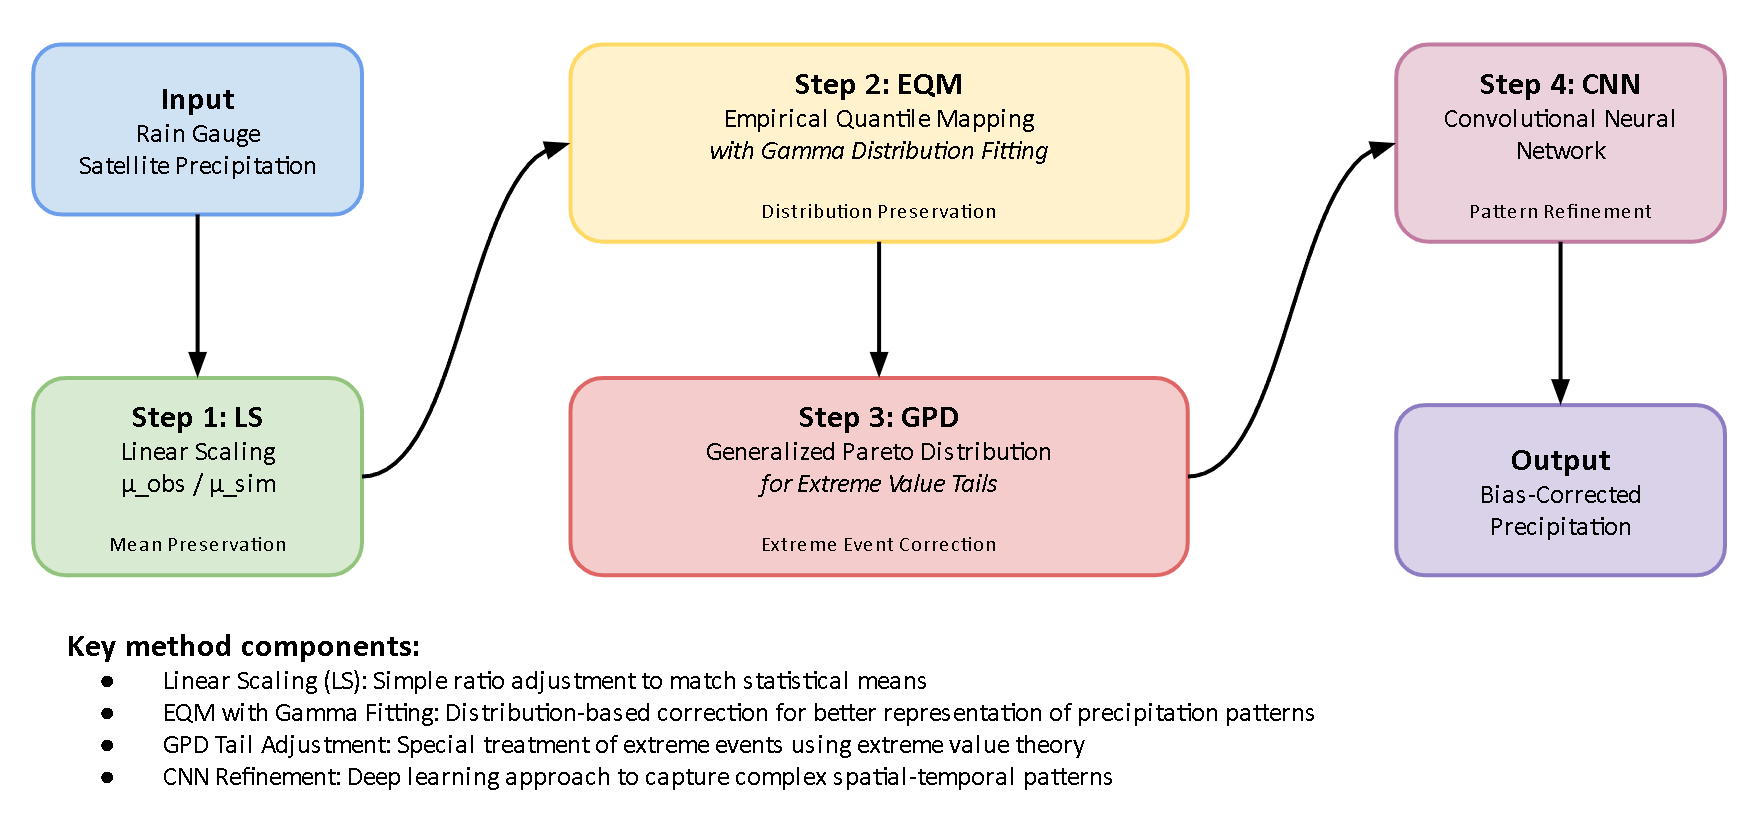
\includegraphics[width=\textwidth]{images/fig02_workflow.png}
\caption{Overview of the hybrid bias correction workflow integrating Linear Scaling (LS), Empirical Quantile Mapping (EQM) with Gamma fitting, Generalized Pareto Distribution (GPD) tail adjustment, and Convolutional Neural Network (CNN) refinement.\label{fig2}}
\end{figure}

\textbf{Stage 1: Linear Scaling}

Linear Scaling corrects the systematic mean bias by applying a
multiplicative factor derived from the ratio of reference to satellite
mean precipitation. For each dekad, the scaling factor \(C_{LS}\) is
computed as:

\begin{equation}C_{LS} = \frac{\bar{P}_{ref}}{\bar{P}_{sat}}\end{equation}

where \(\bar{P}_{ref}\) and \(\bar{P}_{sat}\) are the mean daily
precipitation of the CPC-UNI reference and IMERG-L satellite datasets,
respectively, pooled over the same dekadal period across all years. The
corrected precipitation is:

\begin{equation}P_{LS} = P_{sat} \cdot C_{LS}\end{equation}

Grid cells where the satellite mean is zero are left unchanged (scaling
factor set to unity). Following the dual-resolution strategy described
in Section 3.2, the CPC-UNI dekadal mean \(\bar{P}_{ref}\) is computed
at the native \(0.5^{\circ}\) grid and bilinearly interpolated to
\(0.1^{\circ}\) before computing \(C_{LS}\).

This produces a spatially smooth scaling field that transitions
gradually across CPC-UNI cell boundaries, rather than exhibiting the
stepwise jumps that would result from computing the mean on the
regridded product. This step aligns the first moment of the
precipitation distribution prior to distributional corrections.

\textbf{Stage 2: Empirical Quantile Mapping with Gamma Distribution
Fitting (EQM)}

Empirical Quantile Mapping aligns the full cumulative distribution
function (CDF) of the LS-corrected satellite precipitation to that of
the reference observations. To improve the stability and smoothness of
the CDFs, particularly in regions with limited sample sizes, gamma
distributions are fitted to the precipitation data prior to mapping.
Gamma parameters (shape \(k\) and scale \(\theta\)) are estimated using
maximum likelihood estimation (MLE) with the location parameter fixed at
zero to ensure physical validity of non-negative precipitation values
\cite{ref15}. The quantile correction for each satellite precipitation value
\(P_{LS}\) is performed by:

\begin{equation}P_{EQM} = F_{ref}^{-1}\left( F_{sat}\left( P_{LS} \right) \right)\end{equation}

where \(F_{sat}\) and \(F_{ref}\) denote the fitted gamma CDFs of the
satellite and reference datasets, respectively, and \(F_{ref}^{-1}\) is
the inverse CDF (quantile function) of the reference distribution.

The IMERG-side gamma CDF (\(F_{sat}\)) is fitted independently at each
\(0.1^{\circ}\) pixel, preserving the full spatial detail of the
satellite product. The CPC-UNI-side gamma CDF (\(F_{ref}\)) is fitted at
the native \(0.5^{\circ}\) resolution, where each cell contains a
statistically independent time series of gauge-analyzed values. The
resulting gamma parameters (shape \(k_{ref}\) and scale
\(\theta_{ref}\)) are then bilinearly interpolated to the
\(0.1^{\circ}\) IMERG grid.

This dual-resolution fitting strategy follows the BCSD principle
\cite{ref23}: by fitting at the resolution where independent information
exists and spatially disaggregating the fitted parameters, the quantile
transfer function varies smoothly across the domain while each parameter
estimate draws on a genuinely distinct observational sample.

\textbf{Dry-day handling.} Because daily tropical precipitation is a
mixed discrete-continuous variable with a large atom at zero, the gamma
distribution is fitted only on wet days (\(P \geq 1\) mm/day) rather
than on the full sample. Fitting a gamma to the mixed sample would bias
the shape parameter toward zero and distort the mapped quantiles. The
dry-day fraction is handled explicitly at the mapping stage following
the unconditional-CDF construction of Cannon et al.~\cite{ref11}. Let
\(p_{dry}^{sat}\) and \(p_{dry}^{ref}\) denote the satellite and
reference dry-day probabilities estimated at each pixel from the
empirical sample. For a satellite wet-day value \(P_{LS} \geq 1\)
mm/day, the unconditional quantile position is
\begin{equation}y = p_{dry}^{sat} + (1 - p_{dry}^{sat}) \cdot F_{sat}^{wet}(P_{LS}),\end{equation}
where \(F_{sat}^{wet}\) is the gamma CDF fitted on wet values only. The
reference quantile is then obtained from the analogous reference
unconditional CDF, with values falling below \(p_{dry}^{ref}\) mapped to
zero. This construction preserves the reference dry-day frequency by
design and prevents satellite drizzle from being mapped to spurious
low-intensity wet-day values.

\textbf{Stage 3: Generalized Pareto Distribution (GPD) Tail Adjustment}

Extreme precipitation values are modeled separately to preserve the
frequency and magnitude of high-impact events that gamma-based EQM may
underrepresent. Precipitation exceedances above the 80th percentile of
the wet-day sample are fitted using the Generalized Pareto Distribution,
with separate thresholds \(u_{sat}\) and \(u_{ref}\) estimated from the
satellite and reference wet-value distributions, respectively. The 80th
percentile threshold was selected to balance two competing requirements:
a sufficiently large number of exceedances for stable GPD parameter
estimation, and a threshold high enough to isolate genuinely extreme
behavior from the bulk distribution \cite{ref7}. This threshold is
consistent with recommendations for tropical regions with frequent heavy
rainfall, where lower thresholds risk contaminating GPD fits with
moderate rainfall, while higher thresholds yield too few exceedances for
reliable estimation \cite{ref25}.

For precipitation values exceeding threshold \(u\), the exceedances
\(y = P - u\) are modeled using the GPD probability density function:

\begin{equation}f(y) = \frac{1}{\sigma} \left( 1 + \xi \frac{y}{\sigma} \right)^{-(1 + 1/\xi)}\end{equation}

where \(\xi\) is the shape parameter and \(\sigma\) is the scale
parameter. The location parameter is fixed at zero because exceedances
are non-negative by construction; leaving the location free would bias
the fitted tail \cite{ref7}. To improve robustness against data sparsity,
GPD parameters are estimated using \(K\)-fold cross-validation
(\(K = 5\)) with shuffled folds, and the final parameters are averaged
across all folds to reduce sensitivity to individual outliers \cite{ref25}.
Conditional probability mapping is then applied to correct extreme
quantiles. For a satellite value \(P_{sat} > u_{sat}\), the conditional
exceedance probability is computed on the satellite side using its own
threshold,

\begin{equation}p_c = \frac{F_{sat}(P_{sat}) - F_{sat}(u_{sat})}{1 - F_{sat}(u_{sat})},\end{equation}

and the GPD-corrected value is obtained from the reference GPD as

\begin{equation}P_{LSEQM} = u_{ref} + G_{ref}^{-1}(p_c),\end{equation}

where \(G_{ref}^{-1}\) is the inverse GPD fitted to the reference
exceedances and \(u_{ref}\) is the reference wet-value 80th percentile.
Computing \(p_c\) on the satellite side ensures that the
tail-substitution probability chain is internally consistent with the
unconditional gamma CDF used in the body of the distribution, and
maintains continuity at the gamma-GPD boundary.

As with the gamma parameters, the GPD threshold, shape, and scale
parameters for the CPC-UNI reference are fitted at the native
\(0.5^{\circ}\) resolution and bilinearly interpolated to the
\(0.1^{\circ}\) grid. The 99.9th percentile cap is similarly computed at
\(0.5^{\circ}\) and interpolated, maintaining spatial consistency across
all correction stages.

After GPD adjustment, corrected values are capped at the interpolated
99.9th percentile of the reference distribution to prevent physically
unrealistic extremes arising from GPD extrapolation.

\textbf{Stage 4: Deep Learning Refinement (CNN)}

Although the preceding statistical corrections substantially reduce
biases in mean, distribution, and extremes, residual errors in extreme
precipitation pixels often persist due to complex local topographic and
atmospheric processes. To address these remaining biases, a
Convolutional Neural Network (CNN) is employed to refine the corrected
precipitation fields, with its corrections selectively applied to
extreme pixels through alpha-blending.

The CNN is trained separately for each dekadal period, using the
LSEQM-corrected fields as input and CPC-UNI observations as the training
target. This two-stage design means the CNN receives input from the same
statistical domain at both training and inference time, avoiding the
domain shift problem that arises when training directly on raw satellite
data \cite{ref9}.

Each daily precipitation field is independently normalized to \([0, 1]\)
by dividing by its maximum value, allowing the CNN to focus on spatial
pattern learning rather than absolute intensity differences:

\begin{equation}\hat{P}_{i} = \frac{P_{i}}{\max(P_{i})}\end{equation}

The CNN architecture consists of:

\begin{itemize}
\tightlist
\item
  Two convolutional layers (\(3 \times 3\) filters) with 32 and 64
  filters, respectively, using ReLU activation and same-padding;
\item
  Max pooling (\(2 \times 2\)) and dropout regularization after each
  convolutional layer (rates of 0.2 and 0.3);
\item
  A flattening layer followed by a dense layer (128 units, ReLU
  activation) with dropout (rate 0.4);
\item
  A linear output layer reconstructing the corrected precipitation
  field.
\end{itemize}

The model is trained by minimizing the mean squared error (MSE) loss:

\begin{equation}\mathcal{L} = \frac{1}{N} \sum_{i=1}^{N} \left( \hat{P}_{DL,i} - \hat{P}_{ref,i} \right)^2\end{equation}

using the Adam optimizer \cite{ref26}, with an 80/20 training-validation
split. Early stopping with a patience of 5 epochs prevents overfitting,
and a batch size of 64 is used for gradient updates.

The schematic of the CNN refinement architecture, including the
alpha-blending integration, is provided in Figure 3.

\begin{figure}[H]
\centering
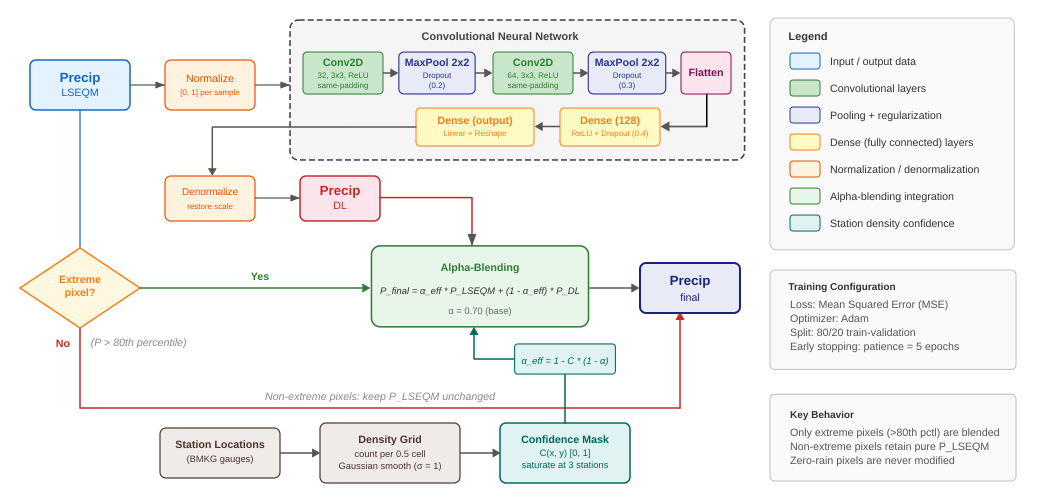
\includegraphics[width=\textwidth]{images/fig03_cnn_pipeline.png}
\caption{CNN refinement pipeline: LSEQM-corrected daily fields are normalized, passed through two convolutional blocks and a Flatten-Dense bottleneck, and reconstructed as a refined field. The refined field is then combined with the LSEQM field through the station-density-modulated alpha-blending step applied only to pixels exceeding the 80th percentile.\label{fig3}}
\end{figure}

\textbf{Alpha-Blending Integration}

The CNN predictions are not applied uniformly across all grid cells.
Instead, an alpha-blending strategy selectively integrates the DL
refinement with the statistical corrections. For each grid cell and time
step, the final corrected precipitation is:

\begin{equation}P_{final} = \alpha_{eff} \cdot P_{LSEQM} + (1 - \alpha_{eff}) \cdot P_{DL}\end{equation}

where \(\alpha_{eff}\) is the effective blending weight. This blending
is applied only to pixels identified as extreme, defined as those where
\(P_{LSEQM}\) exceeds the 80th percentile of the pixel's dekadal
distribution.

Non-extreme pixels retain their LSEQM values without modification, and
pixels with zero precipitation are preserved as zero. The base blending
weight \(\alpha = 0.70\) assigns 70\% weight to the physical-statistical
correction and 30\% to the DL refinement.

\textbf{Station Density Confidence Weighting}

The reliability of the CPC-UNI reference varies spatially depending on
the density of contributing gauge stations. To account for this
heterogeneity, a station density confidence mask modulates the blending
parameter. Gauge station counts per CPC-UNI native grid cell
(\(0.5^{\circ}\)) are computed from the BMKG station network,
Gaussian-smoothed (\(\sigma = 1.0\) grid cells) to prevent sharp
boundaries, then normalized to \([0, 1]\) by dividing by a saturation
count of 3 stations per cell. The confidence mask \(C(x, y)\) modulates
the blending parameter as:

\begin{equation}\alpha_{eff}(x, y) = 1.0 - C(x, y) \cdot (1.0 - \alpha)\end{equation}

This formulation provides a smooth spatial transition: station-dense
areas receive the full DL contribution (\(\alpha_{eff} = 0.70\)), while
station-sparse areas revert toward pure LSEQM
(\(\alpha_{eff} \rightarrow 1.0\)). This approach reduces the risk of
the DL model introducing artifacts in regions where the training target
itself is uncertain \cite{ref27}.

\subsection{Model Evaluation and Quality
Assessment}\label{model-evaluation-and-quality-assessment}

Evaluating bias correction of daily precipitation requires a
multi-metric framework that captures statistical accuracy,
distributional consistency, temporal pattern preservation, and the
representation of extreme events. Daily precipitation exhibits high
temporal variability, frequent dry periods, and intermittent extreme
events, making it more difficult to evaluate than monthly-aggregated
precipitation. A single performance metric cannot capture correction
quality across all relevant dimensions --- event timing, intensity
distribution, dry spell behavior, and extremes --- and this study
therefore employs a structured suite of statistical, categorical,
temporal, and distributional metrics combined with integrated quality
indices, consistent with recommended practice for satellite
precipitation verification \cite{ref14,ref15}.

\paragraph{Nine-Combination Evaluation
Design}\label{nine-combination-evaluation-design}

The evaluation follows a systematic 3 x 3 factorial design (Table 1).
Three reference datasets are used: (1) CPC-UNI, the gauge-based product
used as the training reference for bias correction; (2) IMERG-L, the
uncorrected satellite product; and (3) IMERG-F, the gauge-adjusted IMERG
Final Run product, which serves as an independent benchmark. Each
reference is compared against three correction stages: LS (mean
correction only), LSEQM (mean + distributional correction), and LSEQM+DL
(full hybrid correction). This yields nine reference-test combinations,
enabling three complementary perspectives:

\begin{itemize}
\tightlist
\item
  \textbf{CPC-UNI vs.~corrected products:} Measures absolute correction
  quality against the training reference, assessing how well each stage
  reproduces the gauge-based observations.
\item
  \textbf{IMERG-L vs.~corrected products:} Quantifies improvement
  relative to the uncorrected satellite baseline, isolating the added
  value of bias correction.
\item
  \textbf{IMERG-F vs.~corrected products:} Evaluates performance against
  an independent, gauge-adjusted satellite product that was not used in
  the correction procedure, providing a less circular validation.
\end{itemize}

\textbf{Table 1.} Evaluation matrix: nine reference-test combinations.

\begingroup\small
\begin{longtable}[]{@{}llll@{}}
\toprule
& \textbf{LS} & \textbf{LSEQM} & \textbf{LSEQM+DL} \\
\midrule
\endhead
\bottomrule
\endlastfoot
\textbf{CPC-UNI} & CPC-UNI vs LS & CPC-UNI vs LSEQM & CPC-UNI vs
LSEQM+DL \\
\textbf{IMERG-L} & IMERG-L vs LS & IMERG-L vs LSEQM & IMERG-L vs
LSEQM+DL \\
\textbf{IMERG-F} & IMERG-F vs LS & IMERG-F vs LSEQM & IMERG-F vs
LSEQM+DL \\
\end{longtable}
\endgroup

\subsubsection{Evaluation Metrics}\label{evaluation-metrics}

The performance of each bias correction stage is evaluated using 31
verification metrics organized into four categories: continuous
statistical measures, categorical event detection, temporal pattern
fidelity, and distributional consistency. All metrics are computed at
the pixel level for each dekadal period, enabling spatially explicit
assessment of correction quality.

A wet-day threshold of 1.0 mm/day is applied for all categorical
metrics, consistent with recommendations for tropical regions where
trace precipitation is frequent \cite{ref24}.

Table 2 summarizes the complete metric suite. Formulas for the principal
metrics are provided below; standard definitions for the remaining
metrics follow established references \cite{ref14,ref15}.

Table 2. Summary of verification metrics

\begingroup\small
\begin{longtable}[]{@{}llccc@{}}
\toprule
Category & Metric & Abbreviation & Unit & Perfect Score \\
\midrule
\endhead
\bottomrule
\endlastfoot
Continuous & Relative Bias & RB & ratio & 0 \\
& Pearson Correlation & CORR & -- & 1 \\
& Root Mean Square Error & RMSE & mm/day & 0 \\
& Mean Absolute Error & MAE & mm/day & 0 \\
& Nash-Sutcliffe Efficiency & NSE & -- & 1 \\
& Standard Deviation (ref, test) & STDEV & mm/day & equal \\
& Standard Deviation Ratio & SDR & ratio & 1 \\
& KS Test Statistic / \(p\)-value & KS & -- & 0 / 1 \\
Categorical & Probability of Detection & POD & -- & 1 \\
& False Alarm Ratio & FAR & -- & 0 \\
& Critical Success Index & CSI & -- & 1 \\
& Equitable Threat Score & ETS & -- & 1 \\
Temporal & Frequency of Precipitation Days & FPD & \% & equal \\
& Mean Wet-Day Precipitation & MDWP & mm/day & equal \\
& Maximum Dry Spell Length & DSL & days & equal \\
Distributional & Percentiles (\(Q_{25}\) -- \(Q_{99}\)) & \(Q_{xx}\) &
mm/day & equal \\
\end{longtable}
\endgroup

\textbf{Continuous metrics.}

The Relative Bias measures the proportional difference between test and
reference totals:

\begin{equation}\text{RB} = \frac{\sum_{i=1}^{n} P_{test,i} - \sum_{i=1}^{n} P_{ref,i}}{\sum_{i=1}^{n} P_{ref,i}}\end{equation}

The Pearson Correlation Coefficient quantifies the linear relationship:

\begin{equation}r = \frac{\sum_{i=1}^{n}(P_{ref,i} - \bar{P}_{ref})(P_{test,i} - \bar{P}_{test})}{\sqrt{\sum_{i=1}^{n}(P_{ref,i} - \bar{P}_{ref})^2 \cdot \sum_{i=1}^{n}(P_{test,i} - \bar{P}_{test})^2}}\end{equation}

The Root Mean Square Error and Mean Absolute Error quantify error
magnitude:

\begin{equation}\text{RMSE} = \sqrt{\frac{1}{n} \sum_{i=1}^{n} (P_{test,i} - P_{ref,i})^2}\end{equation}

\begin{equation}\text{MAE} = \frac{1}{n} \sum_{i=1}^{n} |P_{test,i} - P_{ref,i}|\end{equation}

The Nash-Sutcliffe Efficiency provides a normalized measure of
prediction skill relative to the reference mean:

\begin{equation}\text{NSE} = 1 - \frac{\sum_{i=1}^{n}(P_{ref,i} - P_{test,i})^2}{\sum_{i=1}^{n}(P_{ref,i} - \bar{P}_{ref})^2}\end{equation}

NSE values range from \(-\infty\) to 1, where values above 0.5 indicate
satisfactory performance and values below zero indicate that the
reference mean is a better predictor than the corrected product
\cite{ref28,ref29}.

The Standard Deviation is computed independently for both reference and
test datasets using the sample estimator (with Bessel's correction,
\(\text{ddof} = 1\)):

\begin{equation}\sigma = \sqrt{\frac{1}{n-1} \sum_{i=1}^{n} (P_i - \bar{P})^2}\end{equation}

The Standard Deviation Ratio (SDR) quantifies the relative variability
of the corrected product compared to the reference:

\begin{equation}\text{SDR} = \frac{\sigma_{test}}{\sigma_{ref}}\end{equation}

SDR values greater than 1 indicate over-dispersion (excessive
variability), while values less than 1 indicate under-dispersion. A
perfect correction preserves the reference variability
(\(\text{SDR} = 1\)).

\textbf{Categorical metrics.}

Event detection is assessed using the probability of detection, false
alarm ratio, and critical success index, defined in terms of contingency
table entries (hits \(H\), misses \(M\), and false alarms \(F\)):

\begin{equation}\text{POD} = \frac{H}{H + M}, \quad \text{FAR} = \frac{F}{H + F}, \quad \text{CSI} = \frac{H}{H + M + F}\end{equation}

The Equitable Threat Score (ETS) adjusts CSI by removing hits
attributable to random chance:

\begin{equation}\text{ETS} = \frac{H - H_{random}}{H + M + F - H_{random}}, \quad H_{random} = \frac{(H + M)(H + F)}{N}\end{equation}

where \(N\) is the total number of observations. ETS = 0 indicates no
skill beyond random forecasts; ETS = 1 indicates perfect detection
\cite{ref15}.

\textbf{Temporal metrics.}

Three metrics characterize the temporal precipitation patterns. The
Frequency of Precipitation Days (FPD) measures the percentage of days
exceeding the wet-day threshold, computed separately for reference and
test datasets:

\begin{equation}\text{FPD} = \frac{N_{wet}}{N_{valid}} \times 100\end{equation}

where \(N_{wet}\) is the number of days with precipitation \(\geq\) 1.0
mm and \(N_{valid}\) is the total number of valid (non-missing) days.
Comparing FPD between reference and test reveals whether the correction
alters the wet-day frequency.

The Mean Wet-Day Precipitation (MDWP) captures the average intensity on
days that exceed the wet-day threshold:

\begin{equation}\text{MDWP} = \frac{1}{N_{wet}} \sum_{i=1}^{N_{wet}} P_i \quad \text{for } P_i \geq 1.0 \text{ mm/day}\end{equation}

The Maximum Dry Spell Length (DSL) is defined as the longest consecutive
run of days below the wet-day threshold within the evaluation period. It
is computed as:

\begin{equation}\text{DSL} = \max_{j} \{ L_j \}\end{equation}

where \(L_j\) is the length of the \(j\)-th consecutive dry spell. This
metric evaluates whether the bias correction preserves realistic dry
spell persistence, which is relevant for drought monitoring and
agricultural applications.

\textbf{Distributional metrics.}

Six percentiles (\(Q_{25}\), \(Q_{50}\), \(Q_{75}\), \(Q_{90}\),
\(Q_{95}\), \(Q_{99}\)) are computed for both reference and test
datasets to evaluate distributional agreement across the full
precipitation spectrum, with particular emphasis on the upper tail
(\(Q_{90}\) and above) relevant to extreme event assessment. The
two-sample Kolmogorov-Smirnov test evaluates whether the corrected and
reference samples originate from the same underlying distribution:

\begin{equation}D_{KS} = \sup_{x} |F_{test}(x) - F_{ref}(x)|\end{equation}

Metrics are computed in two modes: (1) a timeseries mode producing one
metric grid per year, enabling temporal trend analysis of correction
quality; and (2) a single-dekad mode pooling all years into one
aggregated assessment.

\paragraph{Composite Quality Assessment
Framework}\label{composite-quality-assessment-framework}

While individual metrics provide insight into specific aspects of
correction performance, a composite framework is needed to evaluate the
overall quality of bias-corrected products across multiple dimensions
simultaneously. The Continuous Quality Index (CQI) aggregates multiple
metrics into three principal dimensions: basic statistical quality,
distributional quality, and temporal pattern quality.

\textbf{Basic Statistical Quality Score (BSQS)}

The basic statistical quality score combines three continuous metrics:

\begin{equation}\text{BSQS} = 0.30 \cdot S_{RB} + 0.30 \cdot S_{RMSE} + 0.40 \cdot S_{NSE}\end{equation}

where \(S_{RB} = 1 - \min(|\text{RB}|, 1)\) penalizes both over- and
under-estimation, \(S_{RMSE} = \exp(-\text{RMSE}/5)\) applies
exponential decay normalization, and
\(S_{NSE} = \max(\min(\text{NSE}, 1), 0)\) clips NSE to \([0, 1]\). The
Pearson Correlation Coefficient is not included as a separate component
because it is implicitly captured within the NSE formulation; including
both would introduce double-counting of linear association \cite{ref30}. NSE
receives a higher weight (0.40) as it simultaneously accounts for bias,
variance, and correlation.

\textbf{Distribution Quality Score (DQS)}

The distribution quality score evaluates the preservation of
precipitation intensity distributions across both moderate and extreme
regimes:

\begin{equation}\text{DQS} = 0.45 \cdot S_{extreme} + 0.25 \cdot S_{general} + 0.15 \cdot S_{var} + 0.15 \cdot S_{KS}\end{equation}

where \(S_{extreme}\) is the weighted score across the 90th, 95th, and
99th percentile differences (sub-weights 0.30, 0.30, and 0.40),
\(S_{general}\) captures the 25th, 50th, and 75th percentile differences
(sub-weights 0.30, 0.40, 0.30), and \(S_{var}\) measures the relative
error in the standard deviation ratio. The term \(S_{KS}\) is the
Kolmogorov-Smirnov test \(p\)-value, providing an overall measure of
distributional similarity. The weighting scheme assigns the largest
share (0.45) to extreme percentile matching, reflecting the emphasis on
preserving high-impact events.

Each percentile score is computed as:

\begin{equation}S_{Q_p} = 1 - \min\left(\frac{|Q_{p,test} - Q_{p,ref}|}{Q_{p,ref} + 0.1}, \; 1\right)\end{equation}

and the variability score as:

\begin{equation}S_{var} = 1 - \min(|1 - \text{SDR}|, \; 1)\end{equation}

\textbf{Temporal Quality Score (TQS)}

The temporal quality score assesses the corrected dataset's ability to
reproduce realistic temporal precipitation patterns:

\begin{equation}\text{TQS} = 0.40 \cdot S_{CSI} + 0.30 \cdot S_{event} + 0.30 \cdot S_{spell}\end{equation}

where \(S_{CSI}\) is the Critical Success Index, providing a balanced
joint measure of detection and false alarm performance; \(S_{event}\)
combines Probability of Detection and False Alarm Ratio:

\begin{equation}S_{event} = 0.6 \cdot \text{POD} + 0.4 \cdot (1 - \text{FAR})\end{equation}

and \(S_{spell}\) evaluates the normalized error in maximum dry spell
length:

\begin{equation}S_{spell} = 1 - \min\left(\frac{|\text{DSL}_{test} - \text{DSL}_{ref}|}{\text{DSL}_{ref} + \epsilon}, \; 1\right)\end{equation}

where \(\epsilon = 10^{-6}\) prevents division by zero.

\textbf{Overall Continuous Quality Index (CQI)}

The CQI synthesizes the three component scores into a single normalized
indicator:

\begin{equation}\text{CQI} = 0.35 \cdot \text{BSQS} + 0.35 \cdot \text{DQS} + 0.30 \cdot \text{TQS}\end{equation}

Equal emphasis is placed on basic statistical and distributional quality
(0.35 each), with slightly lower weight for temporal quality (0.30),
reflecting the particular importance of intensity accuracy for climate
risk applications. The CQI is classified into four quality categories
(Table 3).

\textbf{Table 3.} CQI categorical classification

\begingroup\small
\begin{longtable}[]{@{}ccl@{}}
\toprule
Class & CQI Range & Interpretation \\
\midrule
\endhead
\bottomrule
\endlastfoot
Excellent & \(\geq 0.8\) & Correction meets high-performance standards
across all metrics \\
Good & \([0.6, 0.8)\) & Well-performing with minor deficiencies in some
areas \\
Fair & \([0.4, 0.6)\) & Basic improvements achieved but moderate
performance gaps remain \\
Poor & \(< 0.4\) & Substantial deficiencies and limited reliability \\
\end{longtable}
\endgroup

Note: Because the majority of pixels in this study fall within the Fair
range, Figure 6b employs a finer six-tier subdivision (Poor, Marginal,
Fair-Low, Fair-High, Good, Excellent) to reveal spatial structure within
the dominant quality class.

\subsubsection{Confidence Assessment}\label{confidence-assessment}

The confidence score provides an additional layer of information
indicating the reliability of the computed quality metrics. Because the
statistical stability of pixel-level metrics depends on sample size,
metric consistency, and distributional agreement, the confidence
computation is adapted to the evaluation mode.

For the aggregated (single-dekad) evaluation, where sample sizes are
large by design ($\sim$230 daily values pooled across all years):

\begin{equation}C = 0.60 \cdot S_{consistency} + 0.40 \cdot S_{dist}\end{equation}

For the timeseries evaluation, where sample sizes vary per year
($\sim$10 daily values per dekad):

\begin{equation}C = 0.40 \cdot S_{sample} + 0.30 \cdot S_{dist} + 0.30 \cdot S_{consistency}\end{equation}

where \(S_{sample}\) is the fraction of valid (non-missing) time steps,
\(S_{consistency}\) measures agreement among normalized basic metrics
computed as:

\begin{equation}S_{consistency} = 1 - \text{std}\left(\tilde{S}_{RB}, \; \tilde{S}_{NSE}, \; \text{POD}, \; 1 - \text{FAR}\right)\end{equation}

where \(\tilde{S}\) denotes the normalized score (mapped to \([0, 1]\)
where 1 is optimal), and \(S_{dist}\) is the Kolmogorov-Smirnov test
\(p\)-value (higher \(p\)-values indicate greater distributional
similarity and thus higher confidence).

Grid cells or time periods with low confidence scores are flagged,
highlighting regions where the evaluation may be less reliable due to
data limitations or inconsistent correction behavior.

\section{Results and Discussion}\label{results-and-discussion}

Before examining correction performance, it is important to characterize
the starting conditions. The uncorrected IMERG Late Run over Indonesia
exhibits a systematic wet bias against the CPC-UNI reference, with
domain-median relative bias of approximately +15\% during the wet season
(October--March). This bias has a conditional structure: IMERG
overestimates precipitation on days that CPC-UNI classifies as light
rain while simultaneously underestimating moderate-to-heavy events
(Section 4.1.1), a pattern consistent with published IMERG-L evaluations
over the Maritime Continent \cite{ref31,ref32,ref33}. The CPC-UNI reference itself
carries important limitations: at \(0.5^{\circ}\) resolution with 180
contributing stations across Indonesia, gauge density is heavily
concentrated in Java and southern Sumatra (Section 4.6, Figure 10a),
leaving eastern Indonesia (Papua, Maluku, Nusa Tenggara) dependent on
interpolation that may not capture local extremes. The independent BMKG
station network used for validation (171 stations with \(\geq\) 30 valid
days) shares a similar spatial distribution, with station density
highest in Java. This geographic concentration means that domain-median
validation statistics are more representative of conditions in
station-dense western Indonesia than in the data-sparse east --- a
caveat that should be borne in mind when interpreting the results below.

\subsection{Progressive Improvement Across Correction
Stages}

The hybrid framework targets three complementary aspects of satellite
precipitation bias: adjusting values (mean and magnitude), aligning
distributions (statistical shape), and preserving extremes (tail
accuracy). To evaluate whether each correction stage delivers on its
intended objective, domain-wide verification metrics were computed for
the uncorrected IMERG Late Run and the three correction products (LS,
LSEQM, and LSEQM+DL) against the CPC-UNI gauge-based reference. Table 4
organizes the evaluation around these three design objectives,
supplemented by categorical event detection metrics. All values
represent the spatial median across Indonesian land pixels, averaged
over 36 dekadal periods (12 months \(\times\) 3 dekads per month). Ratio
metrics express the corrected product relative to the reference (target
= 1.0).

\begin{landscape}
\textbf{Table 4.} Domain-wide evaluation by correction stage against
CPC-UNI, organized by the three design objectives of the hybrid
framework. Values represent the spatial median across all land pixels,
averaged over all 36 dekadal periods. Ratio metrics express
test/reference. Bold indicates the value closest to the target.

\begingroup\small
\begin{longtable}[]{@{}llllll@{}}
\toprule
Evaluation Objective & Metric & LS & LSEQM & LSEQM+DL & Target \\
\midrule
\endhead
\bottomrule
\endlastfoot
\textbf{Value Adjustment} & Relative Bias & 0.0000 & 0.0697 & 0.0652 &
0 \\
& Std. Dev. Ratio & 0.9707 & 1.1587 & 1.1475 & 1.0 \\
\textbf{Distribution Alignment} & KS \(p\)-value (\%) & 6.56 & 0.00 &
0.00 & 100 \\
& Wet-Day Freq. Ratio & 1.0397 & 0.9466 & 0.9462 & 1.0 \\
& Mean Wet-Day Precip Ratio & 0.9611 & 1.1569 & 1.1519 & 1.0 \\
\textbf{Extreme Preservation} & \(Q_{95}\) Ratio & 0.9459 & 1.1711 &
1.1626 & 1.0 \\
& \(Q_{99}\) Ratio & 0.9669 & 1.2117 & 1.1964 & 1.0 \\
\textbf{Event Detection} & POD & 0.7669 & 0.7069 & 0.7069 & 1.0 \\
& CSI & 0.5890 & 0.5723 & 0.5724 & 1.0 \\
& FAR & 0.2705 & 0.2476 & 0.2475 & 0 \\
\textbf{Temporal Skill} (acknowledged limitation) & Pearson Corr &
0.3430 & 0.3451 & 0.3476 & 1.0 \\
& RMSE (mm/day) & 13.1051 & 14.1797 & 14.0717 & 0 \\
& NSE & $-$0.2728 & $-$0.5479 & $-$0.5241 & 1.0 \\
\end{longtable}
\endgroup
\end{landscape}

The results reveal a pattern consistent with the design intent of each
correction stage. Linear Scaling drives the domain-wide relative bias
against CPC-UNI to zero by construction, since \(C_{LS}\) is defined
exactly as the ratio of reference to satellite dekadal means; the
standard deviation ratio of \(\approx 0.97\) indicates that a uniform
multiplicative rescaling leaves the distributional shape essentially
unchanged. The addition of EQM with GPD tail adjustment (LSEQM) then
modifies the shape of the distribution: the wet-day-mean ratio moves
from 0.96 (LS) to 1.16 and the \(Q_{95}\)/\(Q_{99}\) ratios move from
below unity to above unity (Table 4). These shifts are intentional
rather than deficient: LS by construction under-represents wet-day
intensity because it also rescales drizzle days upward, and EQM with a
wet-day-only gamma fit plus explicit dry-day handling (Section 3.3)
lifts the conditional wet-day distribution back toward the reference.
The apparent ``overshoot'' at the upper percentiles against CPC-UNI is
analyzed further in Sections 4.5 and 4.8.5, where independent BMKG
station validation shows that the LSEQM+DL \(Q_{99}\) ratio lands at
1.01 against gauge observations, compared with 0.71 for LS --- the
opposite direction from the CPC-UNI-based assessment.

The CNN refinement (LSEQM+DL) provides targeted adjustment at the
extreme end: the standard deviation ratio moves slightly closer to unity
and \(Q_{95}\)/\(Q_{99}\) move modestly toward the reference. The CNN
effect is intentionally small, reflecting the conservative
alpha-blending design (\(\alpha = 0.70\) applied only to extreme
pixels), which limits the DL contribution to at most 30\% of the
correction signal and only where the station density confidence mask
permits.

Event detection shows a trade-off inherent to distributional correction:
POD and CSI shift marginally across correction stages (Table 4),
reflecting the fact that quantile mapping adjusts wet-day precipitation
magnitudes and can move marginal events above or below the 1 mm/day
detection threshold. FAR remains essentially unchanged, indicating that
the redistribution of values does not systematically inflate false
alarms.

An important characteristic of distributional bias correction methods is
that they adjust marginal distributions without modifying the temporal
sequencing of satellite estimates \cite{ref34,ref11}. Accordingly, pixel-level
temporal accuracy metrics show limited change across correction stages:
Pearson correlation remains at approximately 0.35, RMSE at approximately
13 mm/day, and NSE remains negative (approximately \(-0.3\)) for all
methods. These values reflect the inherent difficulty of reproducing
gauge-interpolated daily precipitation fields at 0.1\(^{\circ}\)
resolution rather than a deficiency of the correction framework. The
method is designed to produce climatologically unbiased rainfall fields
with correct distributional properties --- adjusting values, aligning
distributions, and preserving extremes --- rather than to improve
day-to-day prediction skill at the pixel level.

To provide a compact visual summary of these multi-dimensional
performance characteristics, Figure 4 presents Taylor diagrams \cite{ref35}
comparing all evaluated products against independent BMKG station
observations, stratified by monsoon regime. The diagram simultaneously
displays three complementary statistics: Pearson correlation (angular
position), normalized standard deviation (radial distance), and centered
RMSE (gray dashed contours). A product that perfectly reproduces the
observed variability would coincide with the reference point at
correlation = 1.0 and normalized standard deviation = 1.0.

The seasonal stratification reveals that the method ordering is stable
across both monsoon regimes. In both wet (October--March) and dry
(April--September) seasons, LS underestimates the observed variability
(median standard deviation ratio of 0.71 and 0.74, respectively), while
LSEQM and LSEQM+DL bring the ratio toward unity (1.03/1.00 in the wet
season, 1.04/1.02 in the dry season). Correlation remains largely
unchanged across correction stages (\(\approx\) 0.22--0.25), confirming
that distributional correction does not modify temporal prediction skill
--- consistent with the theoretical expectation discussed in Section
4.1. CPC-UNI, despite serving as the correction target, does not
coincide with the station reference point (standard deviation ratio
\(\approx\) 0.85), reflecting the interpolation uncertainty inherent to
the gauge analysis at \(0.5^{\circ}\) resolution --- a characteristic
that motivates the independent station validation. IMERG-F, included as
an independent benchmark, sits between the uncorrected IMERG-L and the
CPC-UNI reference, consistent with its gauge-adjusted nature.

\begin{figure}[H]
\centering
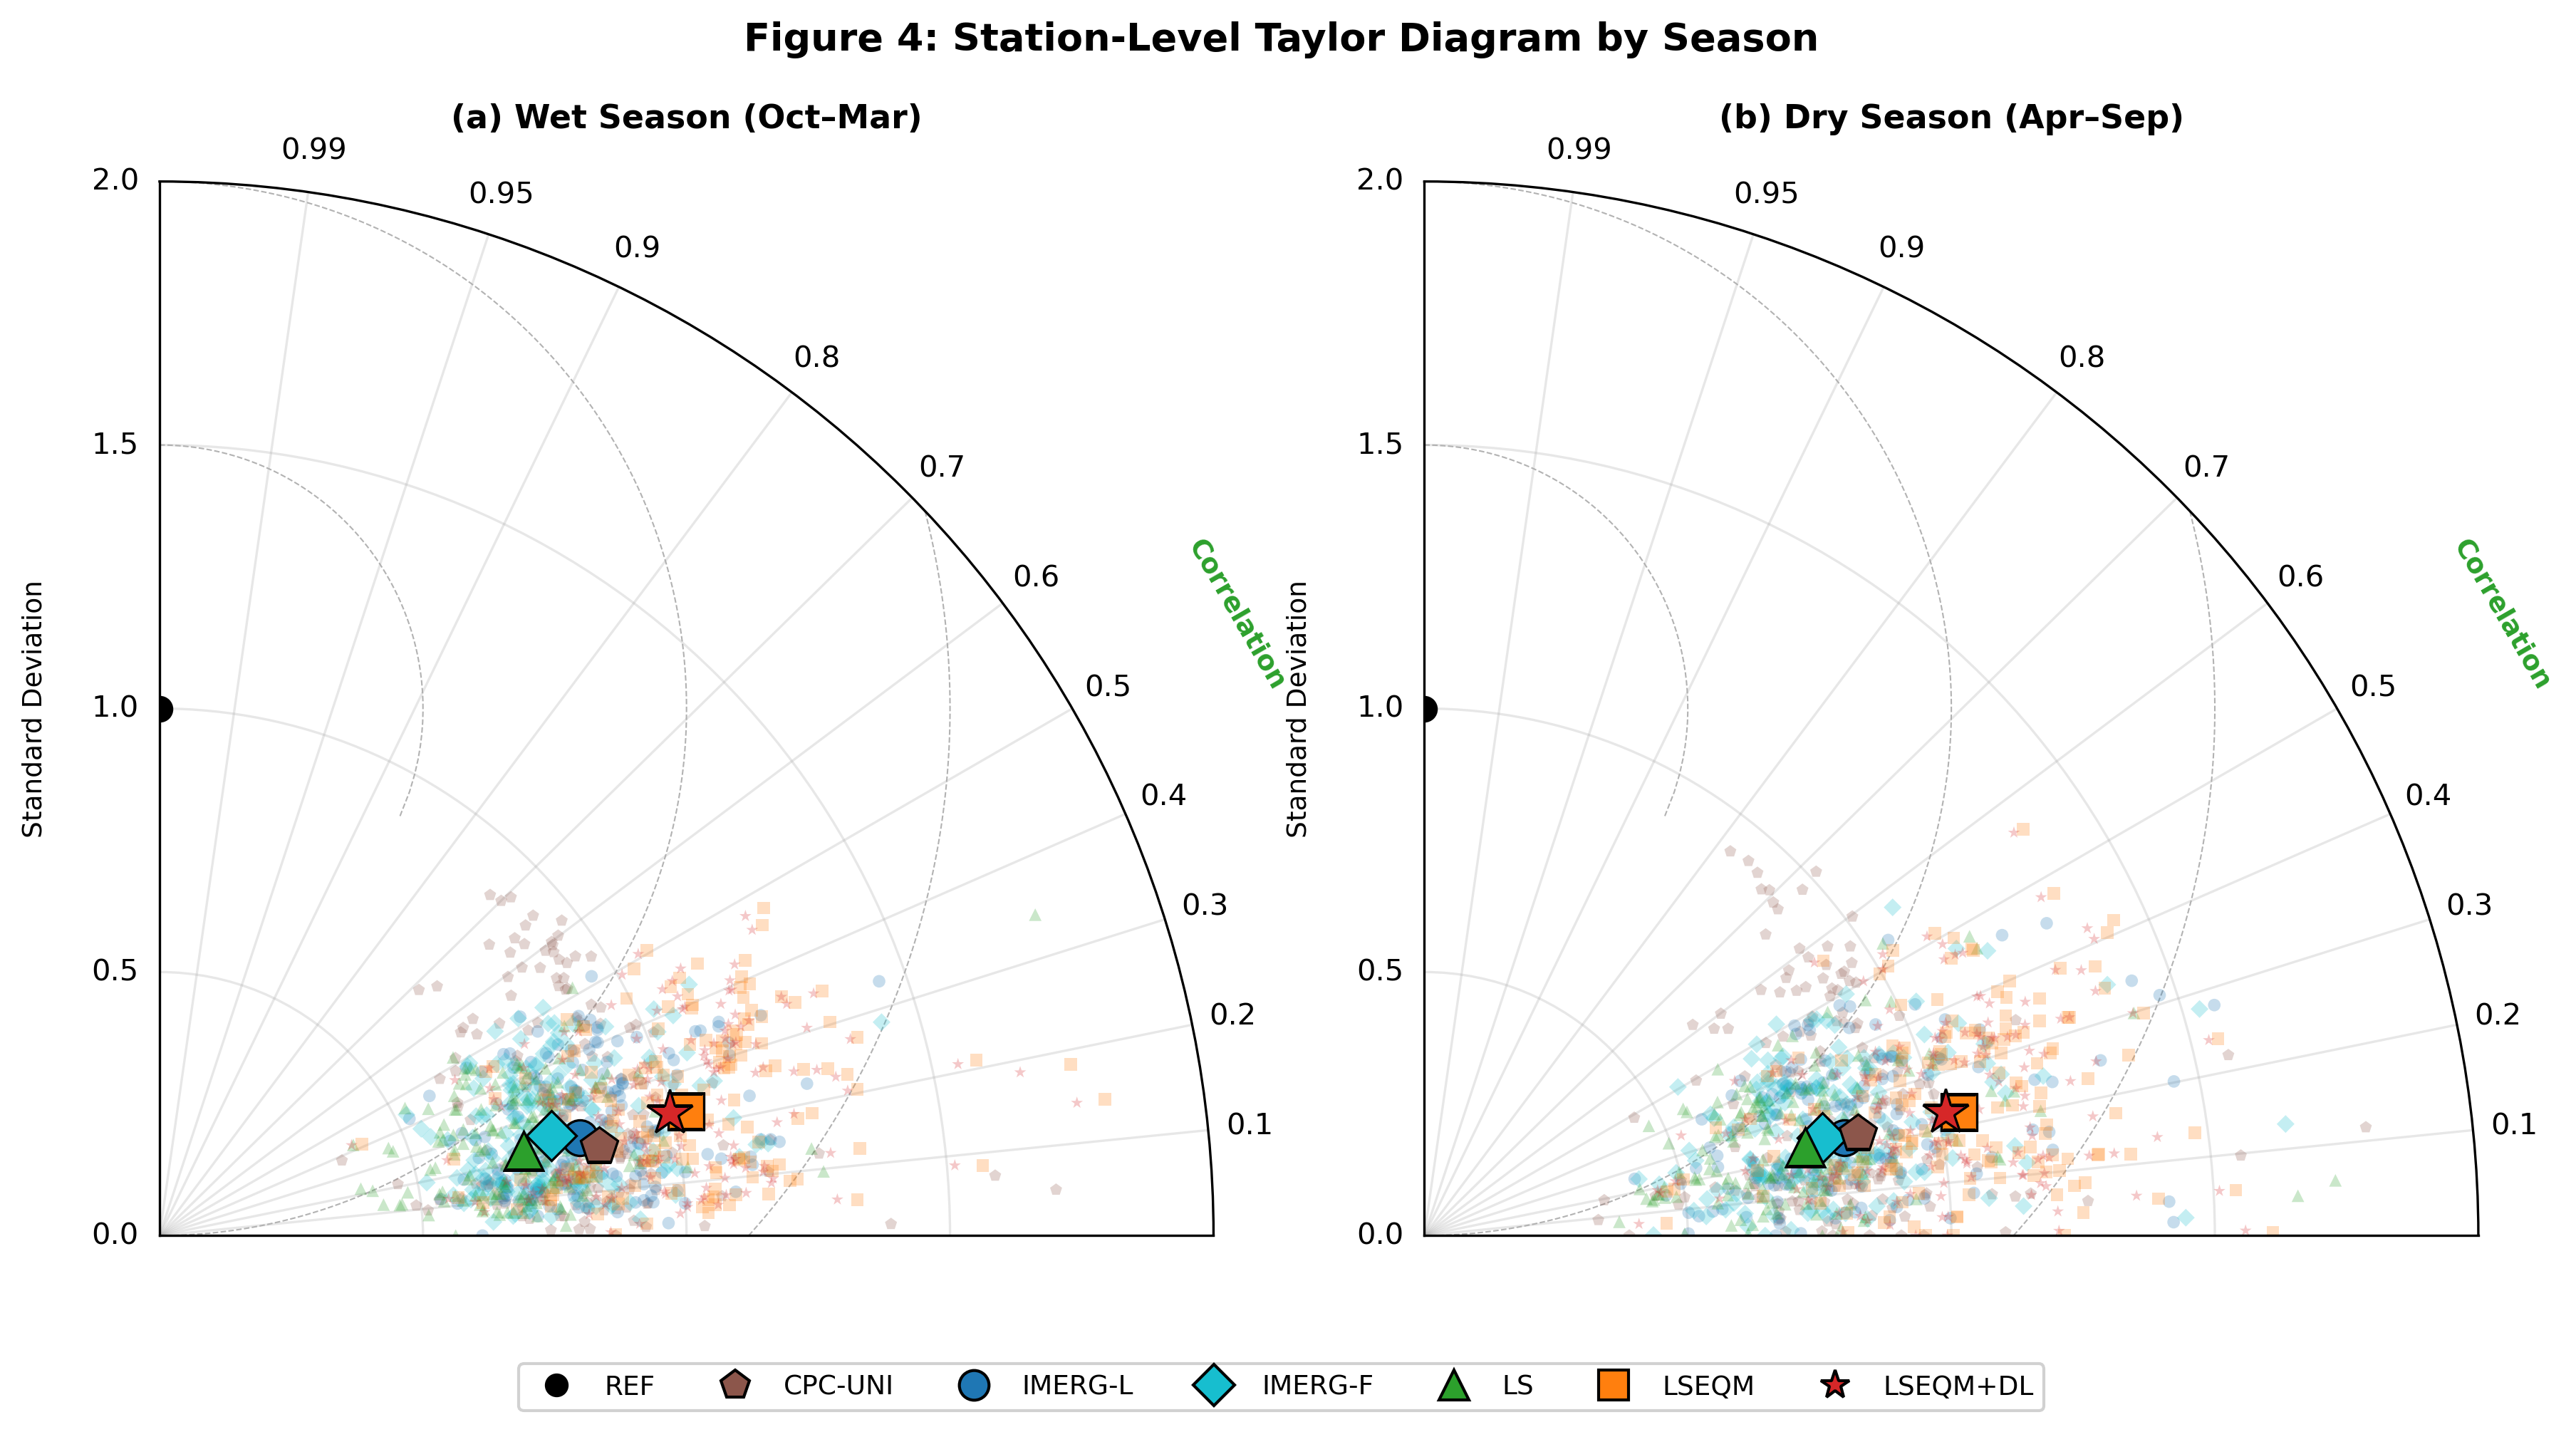
\includegraphics[width=\textwidth]{images/fig04_taylor_by_station.png}
\caption{Taylor diagrams comparing daily precipitation performance against independent BMKG station observations, stratified by (a) wet season (October--March) and (b) dry season (April--September). Products shown: CPC-UNI (brown pentagon), IMERG-L (blue circle), IMERG-F (cyan diamond, included as an independent benchmark), LS (green triangle), LSEQM (orange square), and LSEQM+DL (red star). Large markers indicate the median of per-station normalized statistics; small translucent markers show individual stations. The black circle at correlation = 1.0 and normalized standard deviation = 1.0 represents the station reference. Angular position indicates Pearson correlation, radial distance indicates normalized standard deviation, and gray dashed arcs indicate centered RMSE \cite{ref35}. Statistics are computed from daily paired values across all dekadal periods within each season, for stations with \(\geq\) 30 valid observation days.\label{fig4}}
\end{figure}

The domain-wide averages in Table 4 aggregate regions where the CPC-UNI
reference is well constrained by gauge observations alongside
station-sparse areas where CPC-UNI itself carries substantial
interpolation uncertainty. To disentangle this effect, the analysis was
stratified using the station density confidence mask (Section 4.6). In
station-covered regions (confidence \(C \geq 0.5\), representing 59 of
approximately 78,800 land pixels), the CNN refinement effect is clearly
visible: the standard deviation ratio improves from 1.16 (LSEQM) to 1.05
(LSEQM+DL), and RMSE decreases from 9.0 to 8.3 mm/day. The relative bias
drops from 0.050 (LSEQM) to 0.003 (LSEQM+DL), confirming that the CNN is
most effective where the CPC-UNI reference is well constrained. In
station-sparse regions (\(C < 0.5\)), the LSEQM-to-LSEQM+DL transition
is minimal, reflecting the confidence mask design that reverts toward
purely statistical corrections where few gauges constrain the analysis.
This spatial dependence is explored further in Section 4.6.

\paragraph{Conditional Bias Structure: Per-Pixel Quantile
Decomposition}

The domain-average relative bias reported in Table 4 conceals an
important spatial-conditional structure that is not visible in marginal
summaries. To expose this, a per-pixel decomposition of the relative
bias was performed by partitioning each pixel's time series into three
regions defined on the CPC-UNI reference distribution: R1 (body,
reference values \(\leq Q_{80}\)), R2 (moderate tail,
\(Q_{80} < \text{ref} \leq Q_{99.9}\)), and R3 (extreme, ref
\(> Q_{99.9}\)). The sum-weighted contribution of each region to the
overall domain bias is reported as a percentage-point (pp) share of the
reference total. Table 4b presents this decomposition for January dekad
1 (peak monsoon) using land pixels only.

\textbf{Table 4b.} Per-pixel R1/R2/R3 decomposition of sum-weighted
relative bias against CPC-UNI for January dekad 1, land pixels only.
Contributions are expressed in percentage points of the reference sum
and are additive to the overall RB.

\begingroup\small
\begin{longtable}[]{@{}lrrrr@{}}
\toprule
Field & Overall RB (\%) & R1 contrib (pp) & R2 contrib (pp) & R3 contrib (pp) \\
\midrule
\endhead
\bottomrule
\endlastfoot
Raw IMERG-L & +15.52 & +38.91 & -20.71 & -2.68 \\
LSEQM (this study) & +7.90 & +31.08 & -20.59 & -2.60 \\
\end{longtable}
\endgroup

The decomposition reveals a persistent signature that is conserved
across correction stages: IMERG is systematically \emph{too wet} on days
that CPC-UNI classifies as light-rain days (R1, \(+27\) to \(+39\) pp)
and simultaneously \emph{too dry} on days that CPC-UNI classifies as
moderate-heavy or extreme (R2 \(-21\) pp, R3 \(-2.6\) pp). The two
sign-opposite errors partially cancel in the marginal summary, but at
the pixel-day level they reflect a mismatch in \emph{which days are
heavy where} rather than a mismatch in the marginal distribution of
daily intensities per pixel. This is a conditional, not a marginal,
bias.

A conditional mismatch of this form cannot be removed by univariate
quantile mapping by construction, because quantile mapping adjusts the
marginal CDF of each pixel without modifying the temporal assignment of
values to days. The LSEQM correction visibly flattens R1 (from \(+38.9\)
to \(+31.1\) pp) and leaves R2 and R3 essentially unchanged, consistent
with a marginal correction acting on an underlying conditional error.
The implications of this structure for residual bias attribution are
discussed in Section 4.8.5.

\subsection{Spatial Distribution of Correction
Quality}

While domain-averaged statistics provide a useful summary, they mask
important spatial heterogeneity in correction performance. Figure 5
presents the Continuous Quality Index (CQI) spatial maps for all three
correction stages, computed as the mean CQI across all 36 dekadal
periods to provide a climatological summary of correction quality.

The CQI maps reveal a clear west-to-east gradient in correction quality.
Java, southern Sumatra, and Bali, regions characterized by dense gauge
networks and relatively homogeneous terrain at the CPC-UNI resolution,
consistently achieve CQI values in the Fair to Good range (0.5--0.65)
across all three methods. Eastern Indonesia, including Papua and Maluku,
shows lower CQI values, reflecting both the sparser station coverage of
the CPC-UNI reference and the greater topographic complexity of these
regions. The CQI ranges are {[}0.337, 0.657{]} for LS, {[}0.283,
0.602{]} for LSEQM, and {[}0.285, 0.608{]} for LSEQM+DL.

The domain-median CQI decreases from 0.541 (LS) to 0.505 (LSEQM) and
recovers slightly to 0.508 (LSEQM+DL). This decrease may appear to
contradict the distributional improvements documented in Section 4.1,
but it reflects the composite nature of CQI: the Temporal Quality Score
(TQS), which includes POD and CSI, decreases from 0.666 to 0.648 because
the dry-day frequency matching \cite{ref11} reclassifies some IMERG wet days
as dry (reducing POD from 0.77 to 0.71), while the Basic Statistical
Quality Score (BSQS) decreases from 0.326 to 0.297 (LSEQM) and 0.299
(LSEQM+DL) due to the increase in RMSE that accompanies the wider
corrected distribution. These losses outweigh the gains in Distribution
Quality Score (DQS: 0.686 to 0.656 for LSEQM, recovering to 0.661 for
LSEQM+DL). The CNN refinement partially recovers performance (LSEQM+DL
CQI 0.508 vs LSEQM 0.505), consistent with the targeted spatial
adjustment in station-covered regions.

\begin{figure}[H]
\centering
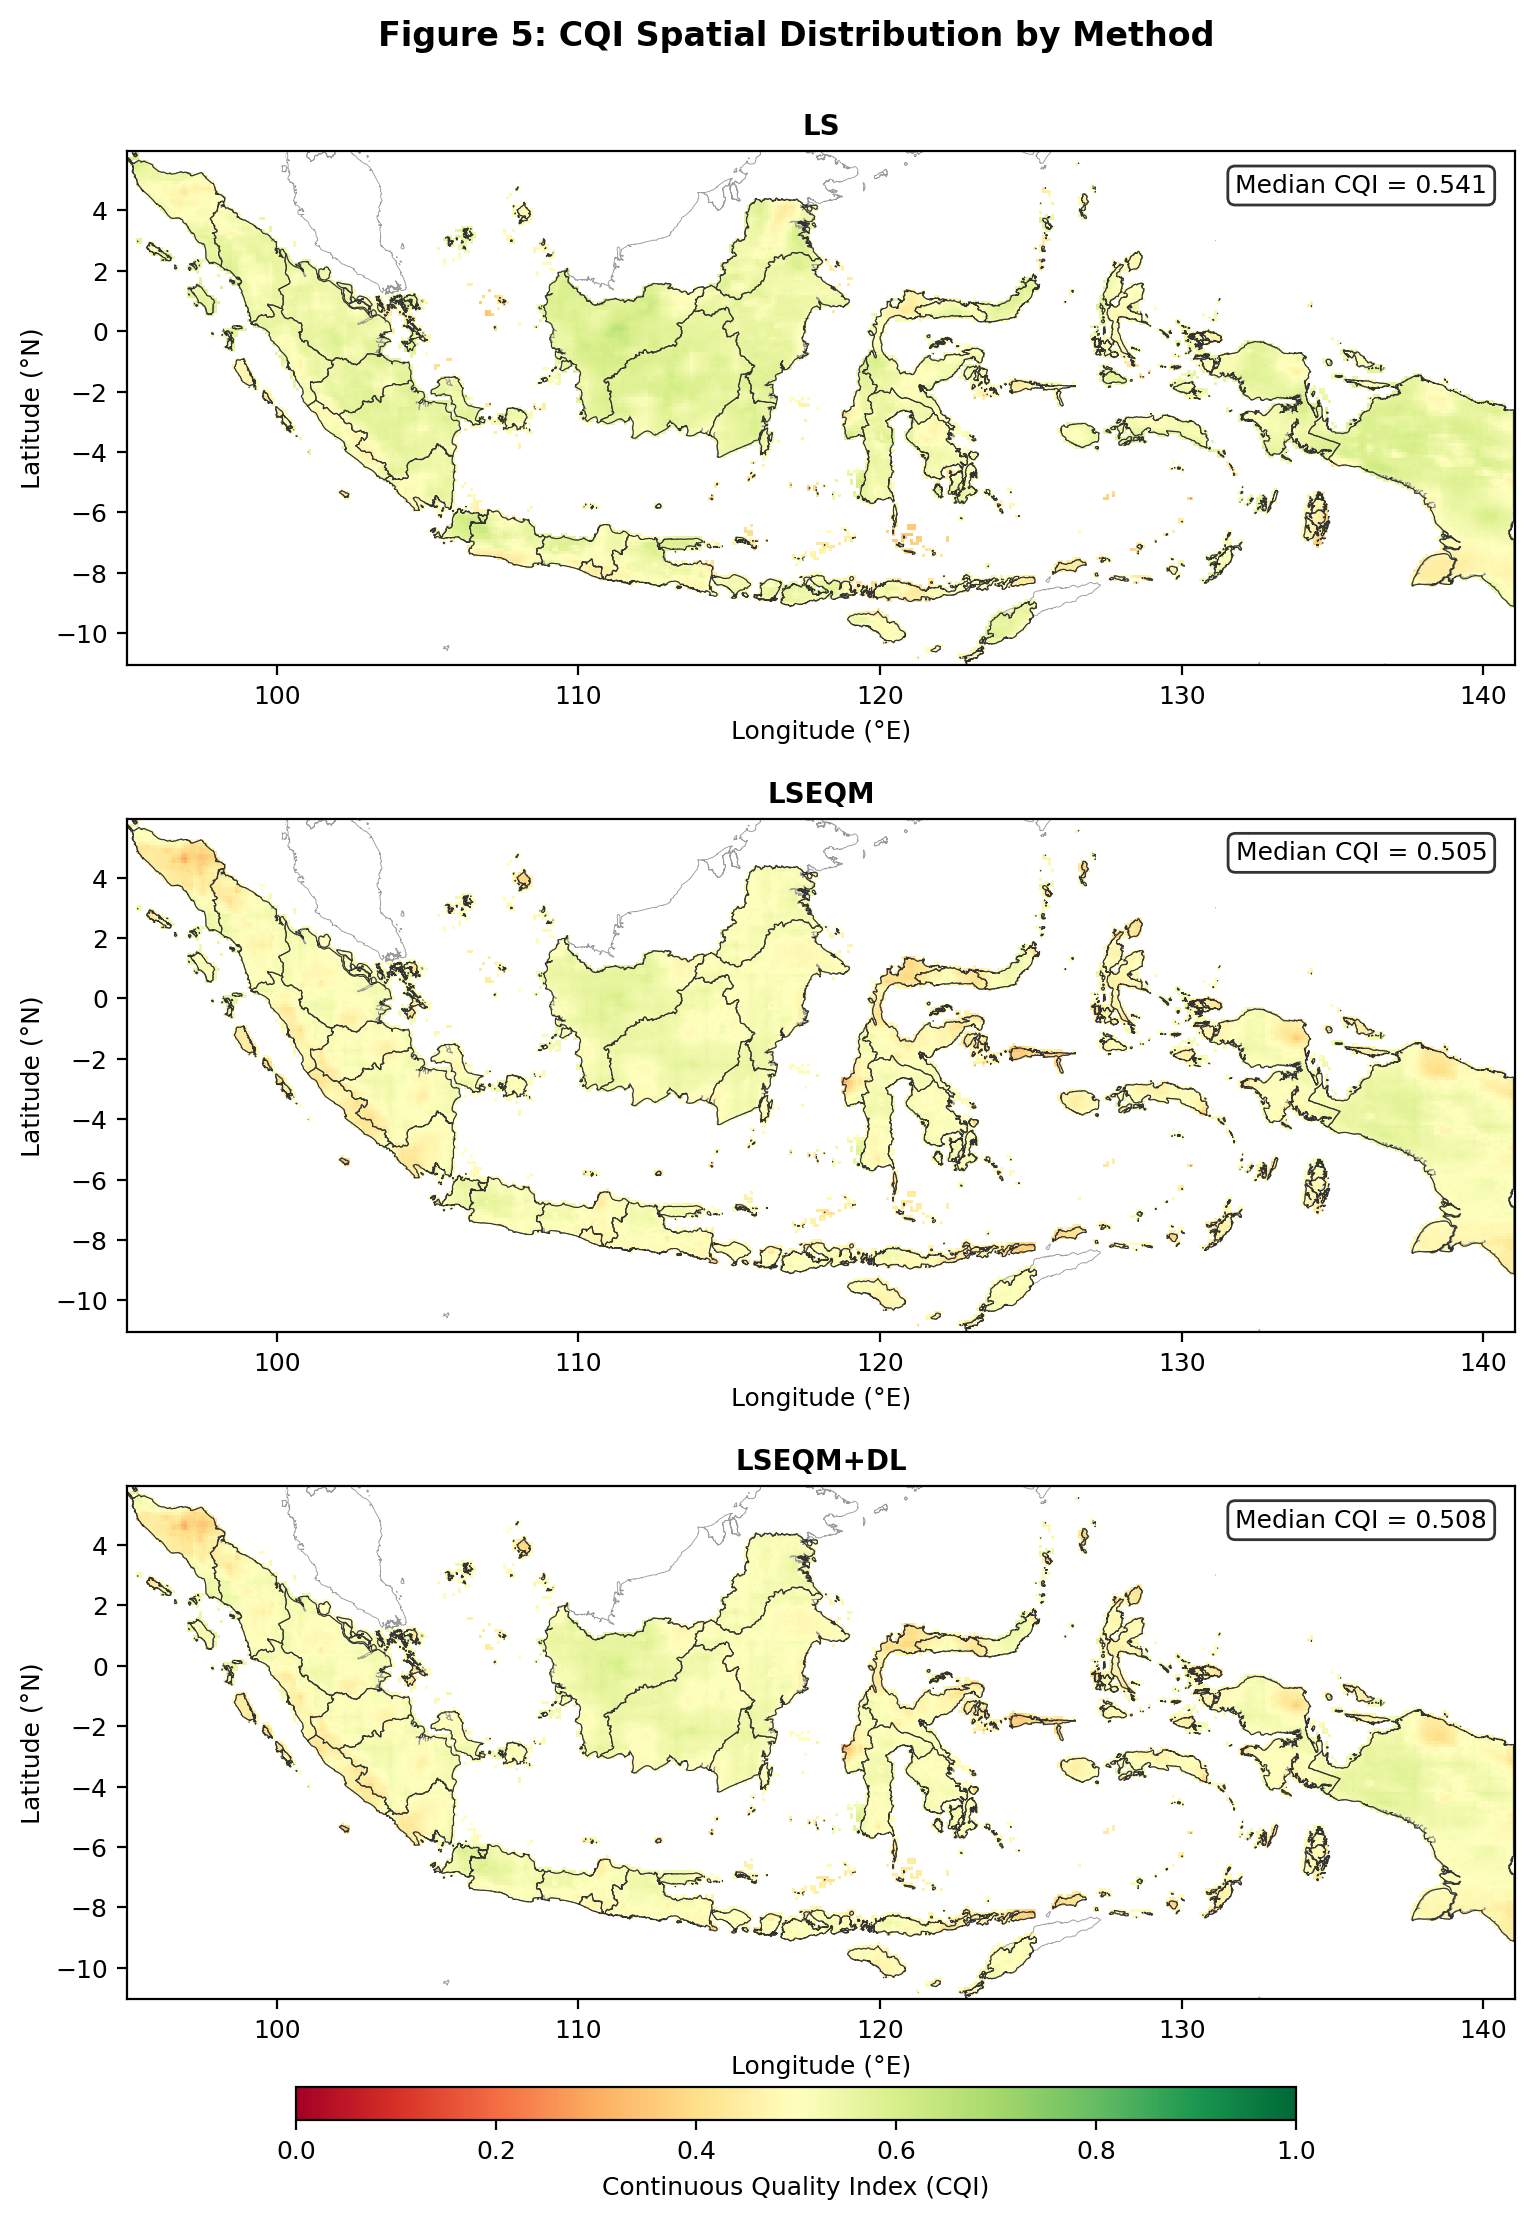
\includegraphics[width=\textwidth]{images/fig05_cqi_spatial.png}
\caption{Spatial distribution of the Continuous Quality Index (CQI) for (a) Linear Scaling, (b) LSEQM, and (c) LSEQM+DL, evaluated against CPC-UNI. Values represent the mean CQI across all 36 dekadal periods. Higher values indicate better agreement with the reference dataset. The color scale ranges from 0 (poor) to 1 (excellent).}\label{fig5}
\end{figure}

Figure 6a presents a smoothed CQI difference map (LSEQM+DL minus LS),
showing a spatially heterogeneous pattern: regions with higher station
density (Java, Bali, southern Sumatra) tend to show modest CQI gains
from the CNN refinement, while the domain majority shows small decreases
driven by the POD/RMSE trade-off discussed above. Figure 6b presents a
six-tier quality classification for LSEQM+DL that subdivides the
dominant Fair range (0.4--0.6) to reveal spatial structure: the majority
of land pixels fall in the Fair-High (0.5--0.6) and Fair-Low (0.4--0.5)
categories, with a clear west-to-east gradient from Fair-High in
station-dense regions to Fair-Low and Marginal (0.3--0.4) in
station-sparse eastern Indonesia. Only 2 pixels reach Good (\(\geq\)
0.6); no pixels achieve Excellent (\(\geq\) 0.7).

\begin{figure}[H]
\centering
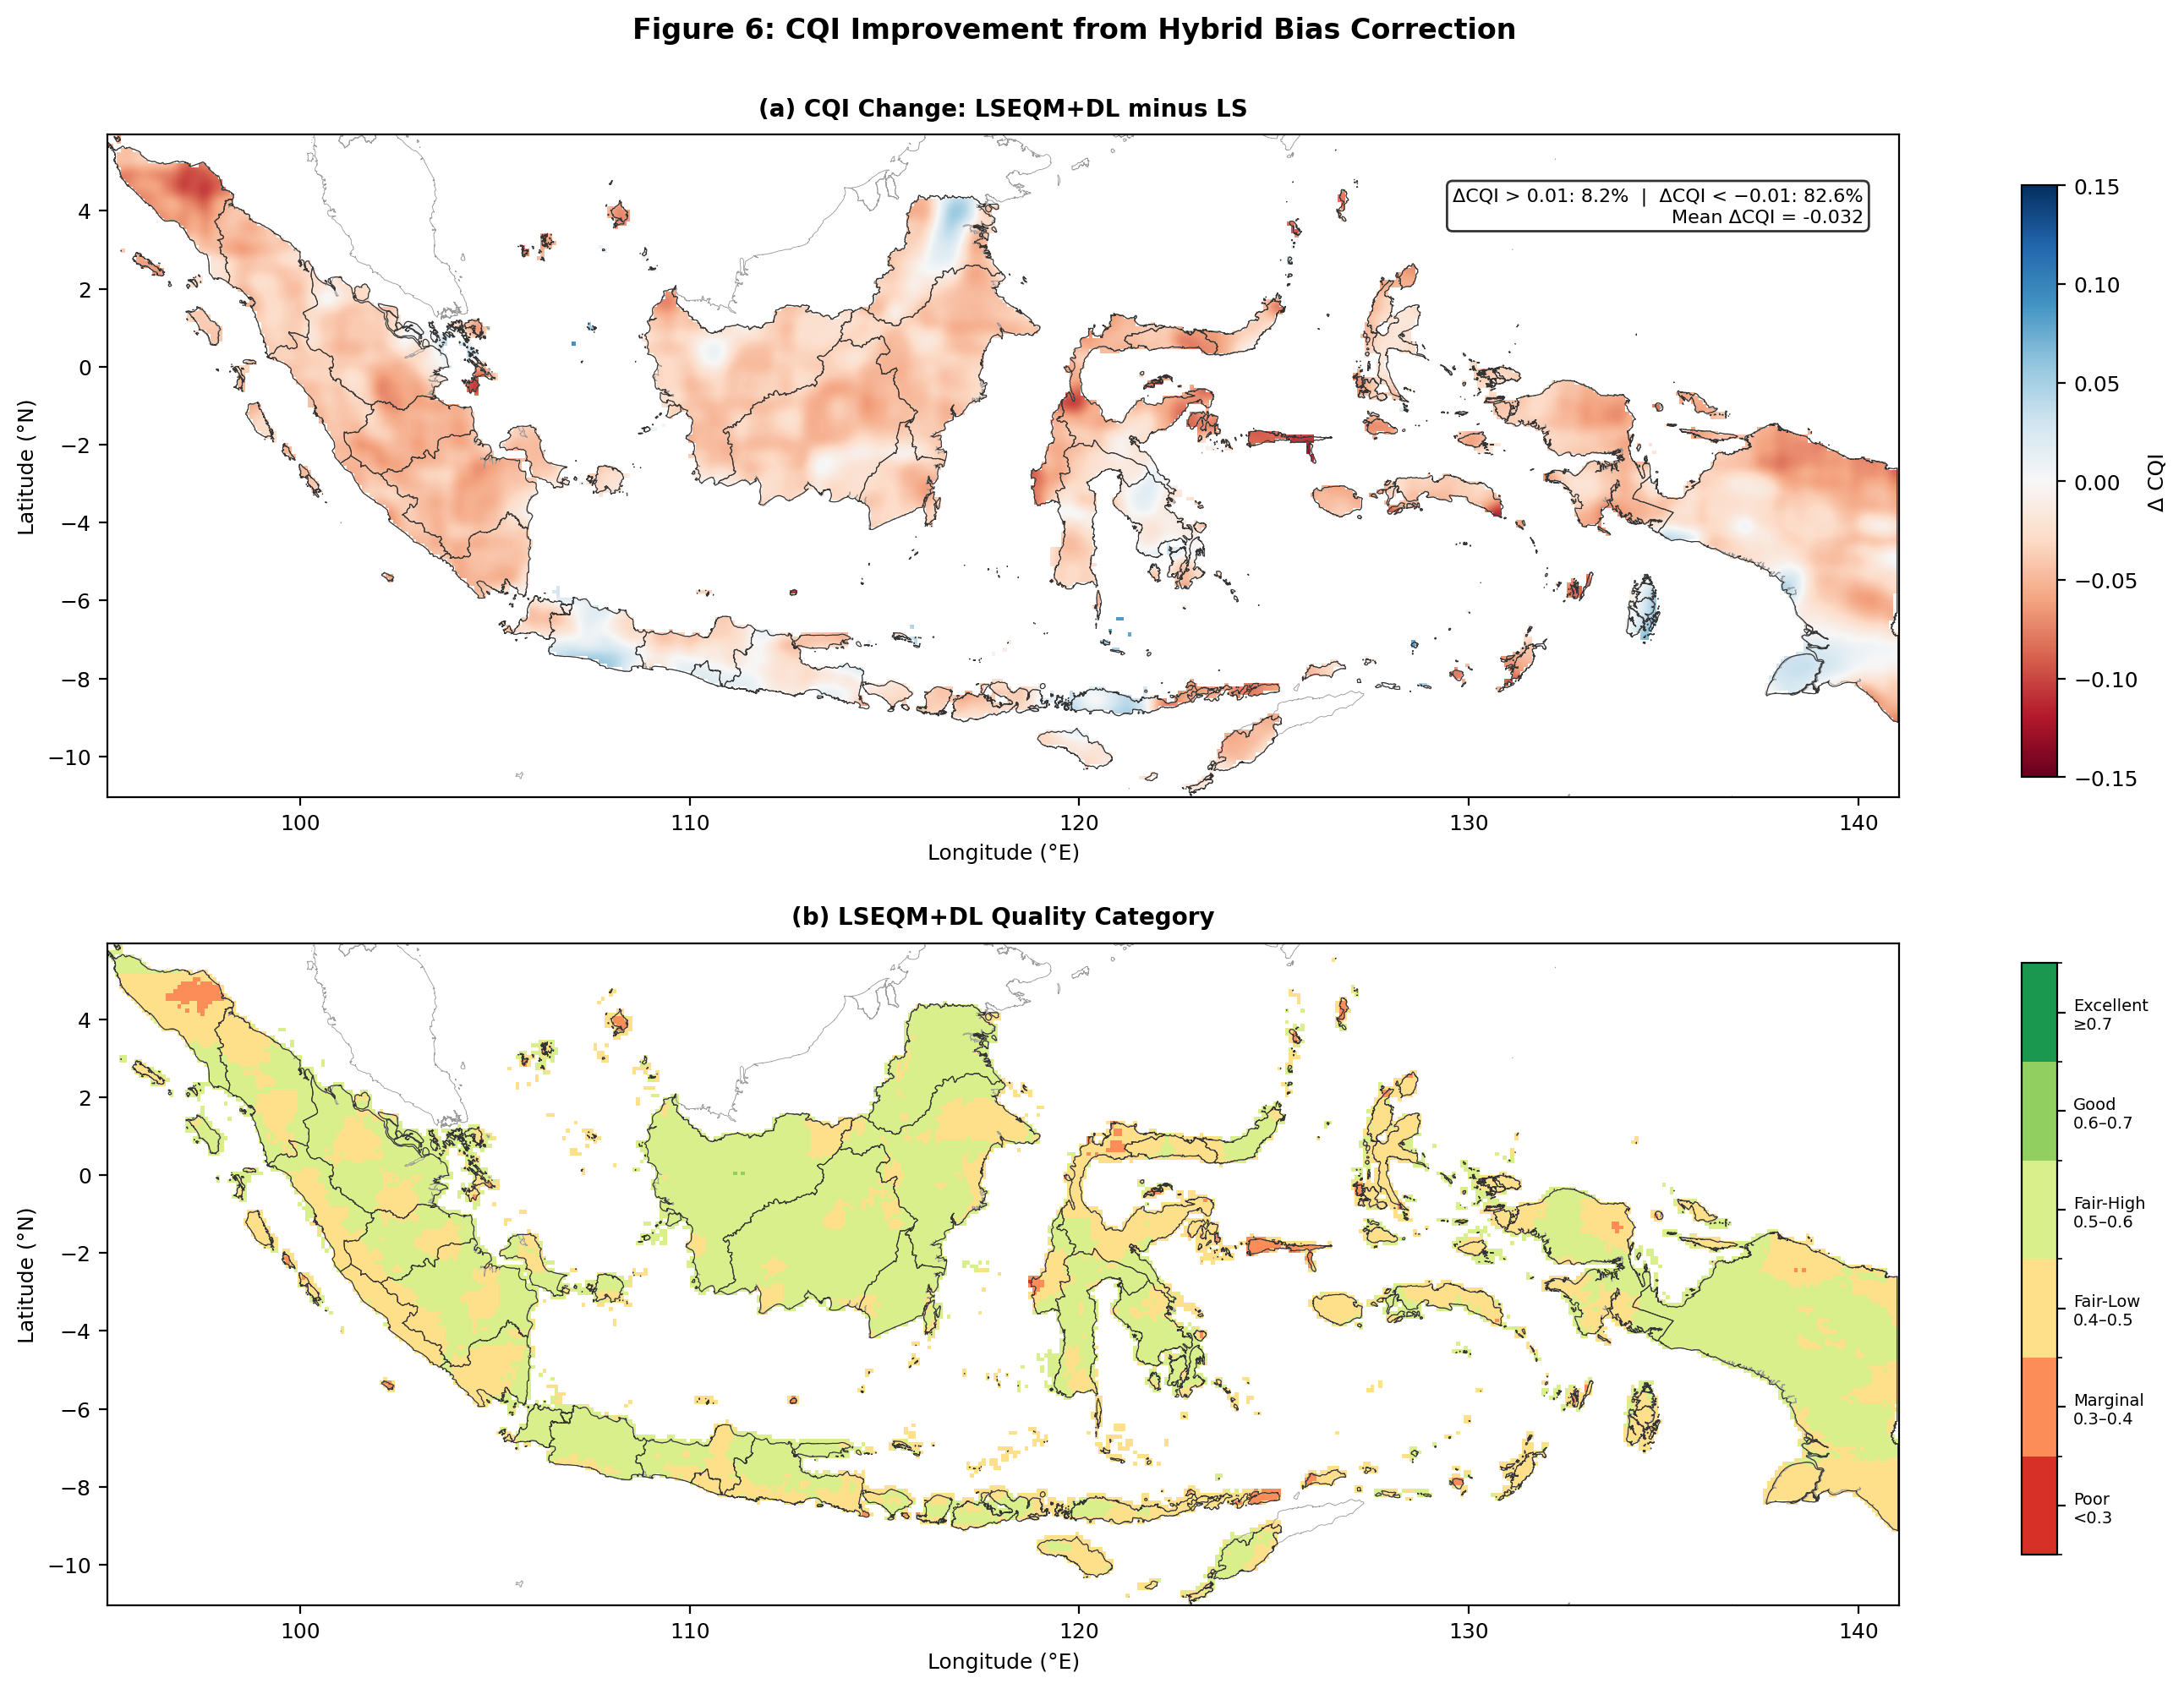
\includegraphics[width=\textwidth]{images/fig06_cqi_improvement.png}
\caption{(a) Smoothed CQI difference map showing the mean difference between LSEQM+DL and LS across all 36 dekadal periods (positive values indicate improvement; Gaussian smoothing with \(\sigma = 1.5\) pixels applied for visual clarity). (b) Six-tier quality classification of LSEQM+DL: Excellent (\(\geq\) 0.7, dark green), Good (0.6--0.7, green), Fair-High (0.5--0.6, yellow-green), Fair-Low (0.4--0.5, yellow), Marginal (0.3--0.4, orange), and Poor (\textless{} 0.3, red).}\label{fig6}
\end{figure}

The spatial pattern of the CQI difference correlates with station
density, a relationship explored further in Section 4.6. The CNN
refinement shows its largest positive contribution in station-dense
regions, indicating that the alpha-blending strategy and station density
confidence mask effectively target the DL contribution where the
reference is well constrained. This CQI result highlights an important
methodological point: composite quality indices that weight event
detection equally with distributional accuracy may undervalue
corrections that deliberately trade wet-day frequency for distributional
fidelity. The independent station validation (Section 4.5) provides the
clearest assessment of the framework's net benefit.

\subsection{Distributional Quality and Extreme Event
Representation}

A central motivation for the hybrid framework is the preservation of
extreme precipitation events \cite{ref46}, which are often attenuated by
standard bias correction methods. Table 5 presents the domain-median
percentile values for the CPC-UNI reference and each correction stage,
spanning from the median (Q50) to the 99th percentile (Q99). Percentiles
are computed from the single-dekad aggregated mode, which pools
approximately 250 daily values per pixel (25 years \(\times\) 10 days
per dekad), providing adequate sample sizes for stable quantile
estimation.

\textbf{Table 5.} Domain-median precipitation percentiles (mm/day) for
the CPC-UNI reference and each correction stage, averaged over all 36
dekadal periods. Values in parentheses indicate the relative error
against the reference.

\begingroup\small
\begin{longtable}[]{@{}lllll@{}}
\toprule
Percentile & CPC-UNI & LS, \% Err & LSEQM, \% Err & LSEQM+DL, \% Err \\
\midrule
\endhead
\bottomrule
\endlastfoot
\(Q_{25}\) & 0.27 & 0.44 (+62.6\%) & 0.00 ($-$100\%) & 0.00 ($-$100\%) \\
\(Q_{50}\) & 2.22 & 2.62 (+18.0\%) & 1.71 ($-$23.1\%) & 1.71 ($-$23.1\%) \\
\(Q_{75}\) & 8.64 & 8.84 (+2.4\%) & 8.76 (+1.4\%) & 8.76 (+1.4\%) \\
\(Q_{90}\) & 20.22 & 19.47 ($-$3.7\%) & 22.67 (+12.1\%) & 22.61 (+11.8\%) \\
\(Q_{95}\) & 29.80 & 28.47 ($-$4.5\%) & 35.53 (+19.2\%) & 35.27 (+18.4\%) \\
\(Q_{99}\) & 51.31 & 50.59 ($-$1.4\%) & 63.19 (+23.2\%) & 62.46 (+21.7\%) \\
\end{longtable}
\endgroup

Linear Scaling, which applies a uniform multiplicative factor, preserves
the relative percentile structure of the uncorrected satellite field.
Because the IMERG-L upper percentiles happen to sit close to the CPC-UNI
reference in the domain median once the mean is removed, the LS
percentile errors against CPC-UNI appear small at \(Q_{90}\) and above.
This apparent agreement is a statistical coincidence of the
multiplicative rescaling and does not reflect genuine shape correction:
LS systematically under-predicts wet-day intensity and over-predicts
wet-day frequency (Table 4), and these two errors cancel in the upper
percentiles of the pooled sample.

The LSEQM stage modifies the distribution shape through wet-day gamma
mapping and explicit dry-day handling. Against the CPC-UNI reference,
this produces a positive shift in the upper percentiles
(\(Q_{90}\)--\(Q_{99}\)). The direction of this shift is evaluated more
rigorously in Section 4.5 using independent BMKG station observations,
where the \(Q_{99}\) ratio moves from 0.71 (LS) to 1.05 (LSEQM) and 1.01
(LSEQM+DL) --- that is, the shift away from CPC-UNI is a shift
\emph{toward} the gauge ground truth. The residual overshoot observed
against CPC-UNI is interpreted in the context of published IMERG-L
Maritime Continent wet-bias assessments and CPC-UNI gauge undercatch in
Section 4.8.5.

Figure 7 presents the distribution of CQI component scores across all
land pixels, comparing the three correction stages. The box plots reveal
that all three CQI components decrease from LS to LSEQM, with partial
recovery under LSEQM+DL. The BSQS (median: LS 0.326, LSEQM 0.297,
LSEQM+DL 0.299) decreases because the wider corrected distribution
increases RMSE. The DQS (median: LS 0.686, LSEQM 0.656, LSEQM+DL 0.661)
decreases because the CPC-UNI-referenced KS statistic penalizes the
intentional distributional shift toward gauge ground truth. The TQS
(median: LS 0.666, LSEQM 0.648, LSEQM+DL 0.648) decreases because POD
and CSI drop as the dry-day handling \cite{ref11} reclassifies some IMERG
wet days. These component-level patterns explain the overall CQI
decrease discussed in Section 4.2 and underscore the tension between
CPC-UNI-referenced composite indices and the independent station
validation (Section 4.5), which confirms that the distributional
corrections represent genuine improvements.

\begin{figure}[H]
\centering
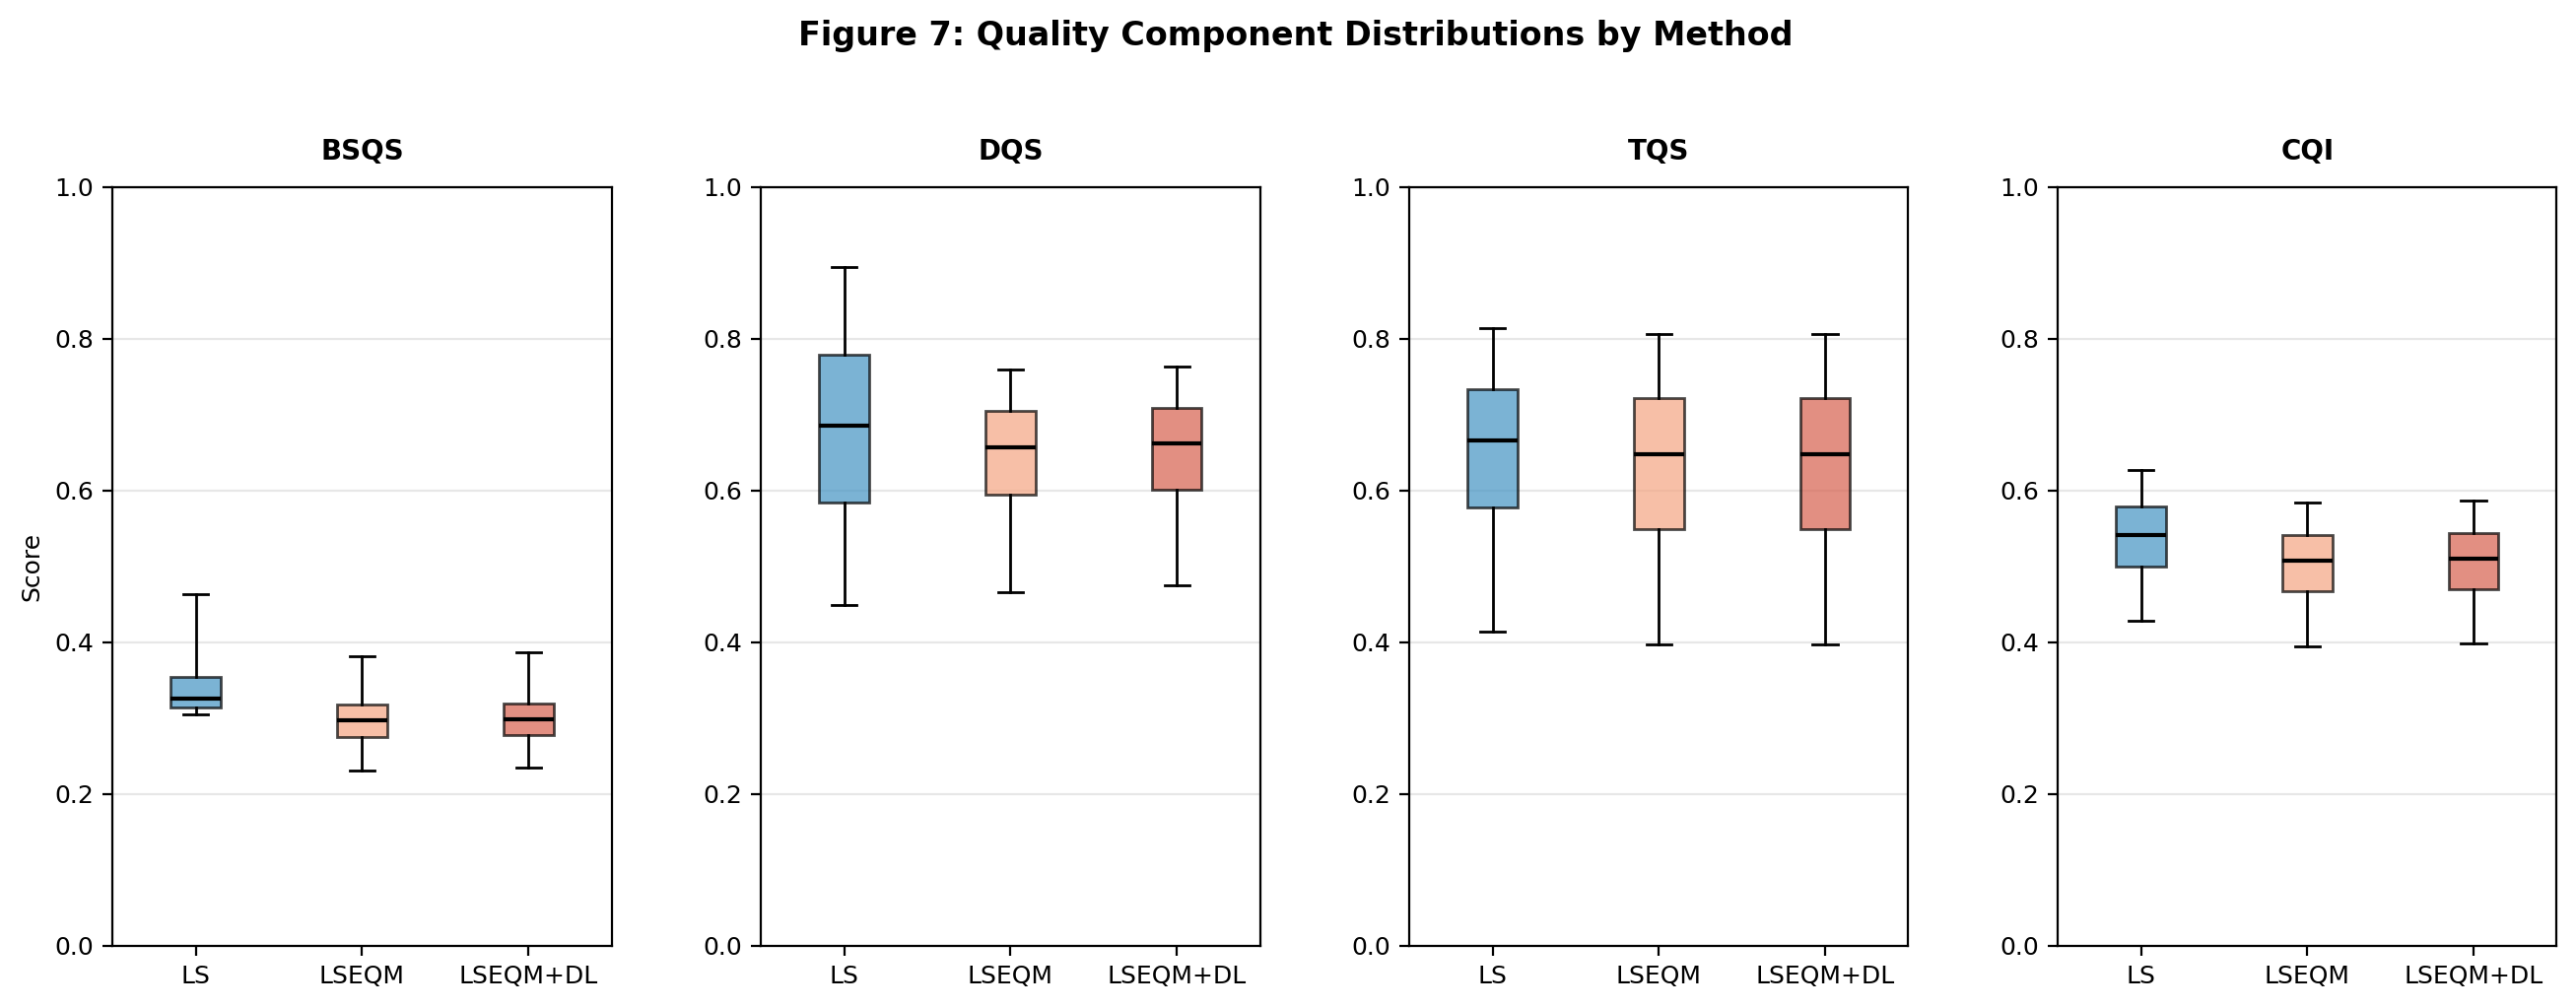
\includegraphics[width=\textwidth]{images/fig07_component_boxplots.png}
\caption{Distribution of CQI component scores across all land pixels for LS (blue), LSEQM (orange), and LSEQM+DL (green): (a) Basic Statistical Quality Score (BSQS), (b) Distribution Quality Score (DQS), (c) Temporal Quality Score (TQS), and (d) overall Continuous Quality Index (CQI). Box plots show the median, interquartile range, and 5th--95th percentile whiskers.}\label{fig7}
\end{figure}

The domain-wide KS \(p\)-values present an apparent paradox: the median
\(p\)-value decreases from 6.56\% (LS) to effectively 0.00\% (LSEQM and
LSEQM+DL), indicating that the corrected distributions are \emph{less}
similar to CPC-UNI than the LS product. This is an expected consequence
of the EQM design: the correction intentionally shifts the satellite
distribution toward independent gauge ground truth (increasing
variability and extreme magnitudes), which moves it further from the
CPC-UNI reference that underestimates these properties. At independent
BMKG stations, the KS \(p\)-value improves from 0.01\% (LS) to 19.07\%
(LSEQM and LSEQM+DL), confirming that the distributional shift
represents genuine improvement when assessed against uncontaminated
ground truth.

\subsection{Cross-Reference
Evaluation}\label{cross-reference-evaluation}

Evaluating bias-corrected products solely against the training reference
(CPC-UNI) risks overly optimistic performance estimates. The evaluation
framework includes cross-reference validation against both the IMERG
Final Run (IMERG-F), a gauge-adjusted satellite product not used in the
correction procedure (Section 3.4.1), and the uncorrected IMERG Late Run
(IMERG-L) as a baseline. This implements the 3 \(\times\) 3 factorial
design described in Table 1, enabling three complementary evaluation
perspectives. IMERG-F is also included in the station-level Taylor
diagram (Figure 4) as an independent benchmark.

Table 6 presents the full evaluation matrix using metrics aligned with
the three-pillar framework. Metrics are summarized as domain-wide
medians averaged over all 36 dekadal periods.

\textbf{Table 6.} Cross-reference evaluation matrix organized by the
three-pillar framework. RB = Relative Bias (value adjustment), SDR =
Std. Dev. Ratio, KS \(p\) = Kolmogorov-Smirnov \(p\)-value (distribution
alignment), \(Q_{99}\)R = 99th-percentile ratio (extreme preservation),
CSI = Critical Success Index (event detection). Bold indicates the value
closest to target per reference group.

\begingroup\small
\begin{longtable}[]{@{}lllllll@{}}
\toprule
Reference & Test & RB & SDR & KS \(p\) (\%) & \(Q_{99}\) Ratio & CSI \\
\midrule
\endhead
\bottomrule
\endlastfoot
CPC-UNI & LS & \textbf{0.0000} & \textbf{0.9707} & \textbf{6.56} &
\textbf{0.9669} & \textbf{0.5890} \\
& LSEQM & 0.0697 & 1.1587 & 0.00 & 1.2117 & 0.5723 \\
& LSEQM+DL & 0.0652 & 1.1475 & 0.00 & 1.1964 & 0.5724 \\
IMERG-F & LS & $-$0.0819 & 0.9549 & \textbf{51.25} & 0.9527 & \textbf{0.9016} \\
& LSEQM & \textbf{$-$0.0093} & 1.1384 & 0.00 & 1.2053 & 0.8574 \\
& LSEQM+DL & $-$0.0140 & \textbf{1.1274} & 0.00 & \textbf{1.1902} & 0.8574 \\
IMERG-L & LS & $-$0.1010 & 0.8990 & \textbf{62.26} & 0.8990 & \textbf{0.9643} \\
& LSEQM & \textbf{$-$0.0279} & 1.0783 & 0.00 & 1.1425 & 0.9117 \\
& LSEQM+DL & $-$0.0326 & \textbf{1.0678} & 0.00 & \textbf{1.1280} & 0.9116 \\
\end{longtable}
\endgroup

The CPC-UNI rows confirm the three-pillar pattern documented in Section
4.1: LS zeroes the relative bias by construction, while LSEQM shifts the
distribution toward the reference with the \(Q_{99}\) ratio moving from
0.97 to 1.21. Against CPC-UNI, LS appears closest to the target for most
metrics, because LS preserves the satellite's distributional shape,
which happens to approximate the CPC-UNI reference.

The IMERG-F rows provide an independent perspective. Because IMERG-F
incorporates gauge data during post-processing, it represents a
higher-quality satellite benchmark. The relative bias against IMERG-F
decreases substantially from $-$0.082 (LS) to $-$0.009 (LSEQM),
indicating that the distributional correction brings the product closer
to the gauge-adjusted satellite estimate. The high CSI values
(0.86--0.90) against IMERG-F reflect the shared satellite retrieval
heritage between IMERG-L and IMERG-F. The standard deviation ratio
against IMERG-F moves from 0.95 (LS) toward 1.13 (LSEQM+DL),
overshooting the IMERG-F variability --- consistent with the
interpretation that LSEQM pushes the distribution beyond the
gauge-adjusted satellite product and toward independent gauge ground
truth (Section 4.5).

The IMERG-L rows quantify the magnitude of correction applied. The
relative bias decreases from $-$0.10 (LS) to $-$0.03 (LSEQM), and
the standard deviation ratio moves from 0.90 toward 1.07, confirming
that the framework systematically increases precipitation variability
and extreme magnitudes relative to the uncorrected satellite baseline.

A consistent pattern across all three reference groups is that the KS
\(p\)-value drops to effectively zero after EQM, reflecting the
intentional distributional shift introduced by quantile mapping. This
shift is confirmed as beneficial by the independent station validation
in Section 4.5.

\subsection{Station-Level Ground Truth
Validation}\label{station-level-ground-truth-validation}

The gridded evaluation in Sections 4.1--4.4 assesses correction
performance against the CPC-UNI reference used during training. The most
rigorous test of the framework employs entirely independent ground
truth. The corrected products were compared against daily precipitation
observations from 171 BMKG (Indonesian Meteorological, Climatological,
and Geophysical Agency) weather stations, which were not used in any
stage of the bias correction procedure. A minimum of 30 valid
overlapping days per station follows WMO guidance for precipitation
verification sample sizes; results are robust to increasing this
threshold to 60 days (up to 169 stations retained per dekad).

Figure 8 presents the spatial distribution of BMKG stations alongside
the per-station standard deviation ratio for the LSEQM+DL product, which
measures how well the corrected product reproduces the observed
precipitation variability at each gauge location.

\begin{figure}[H]
\centering
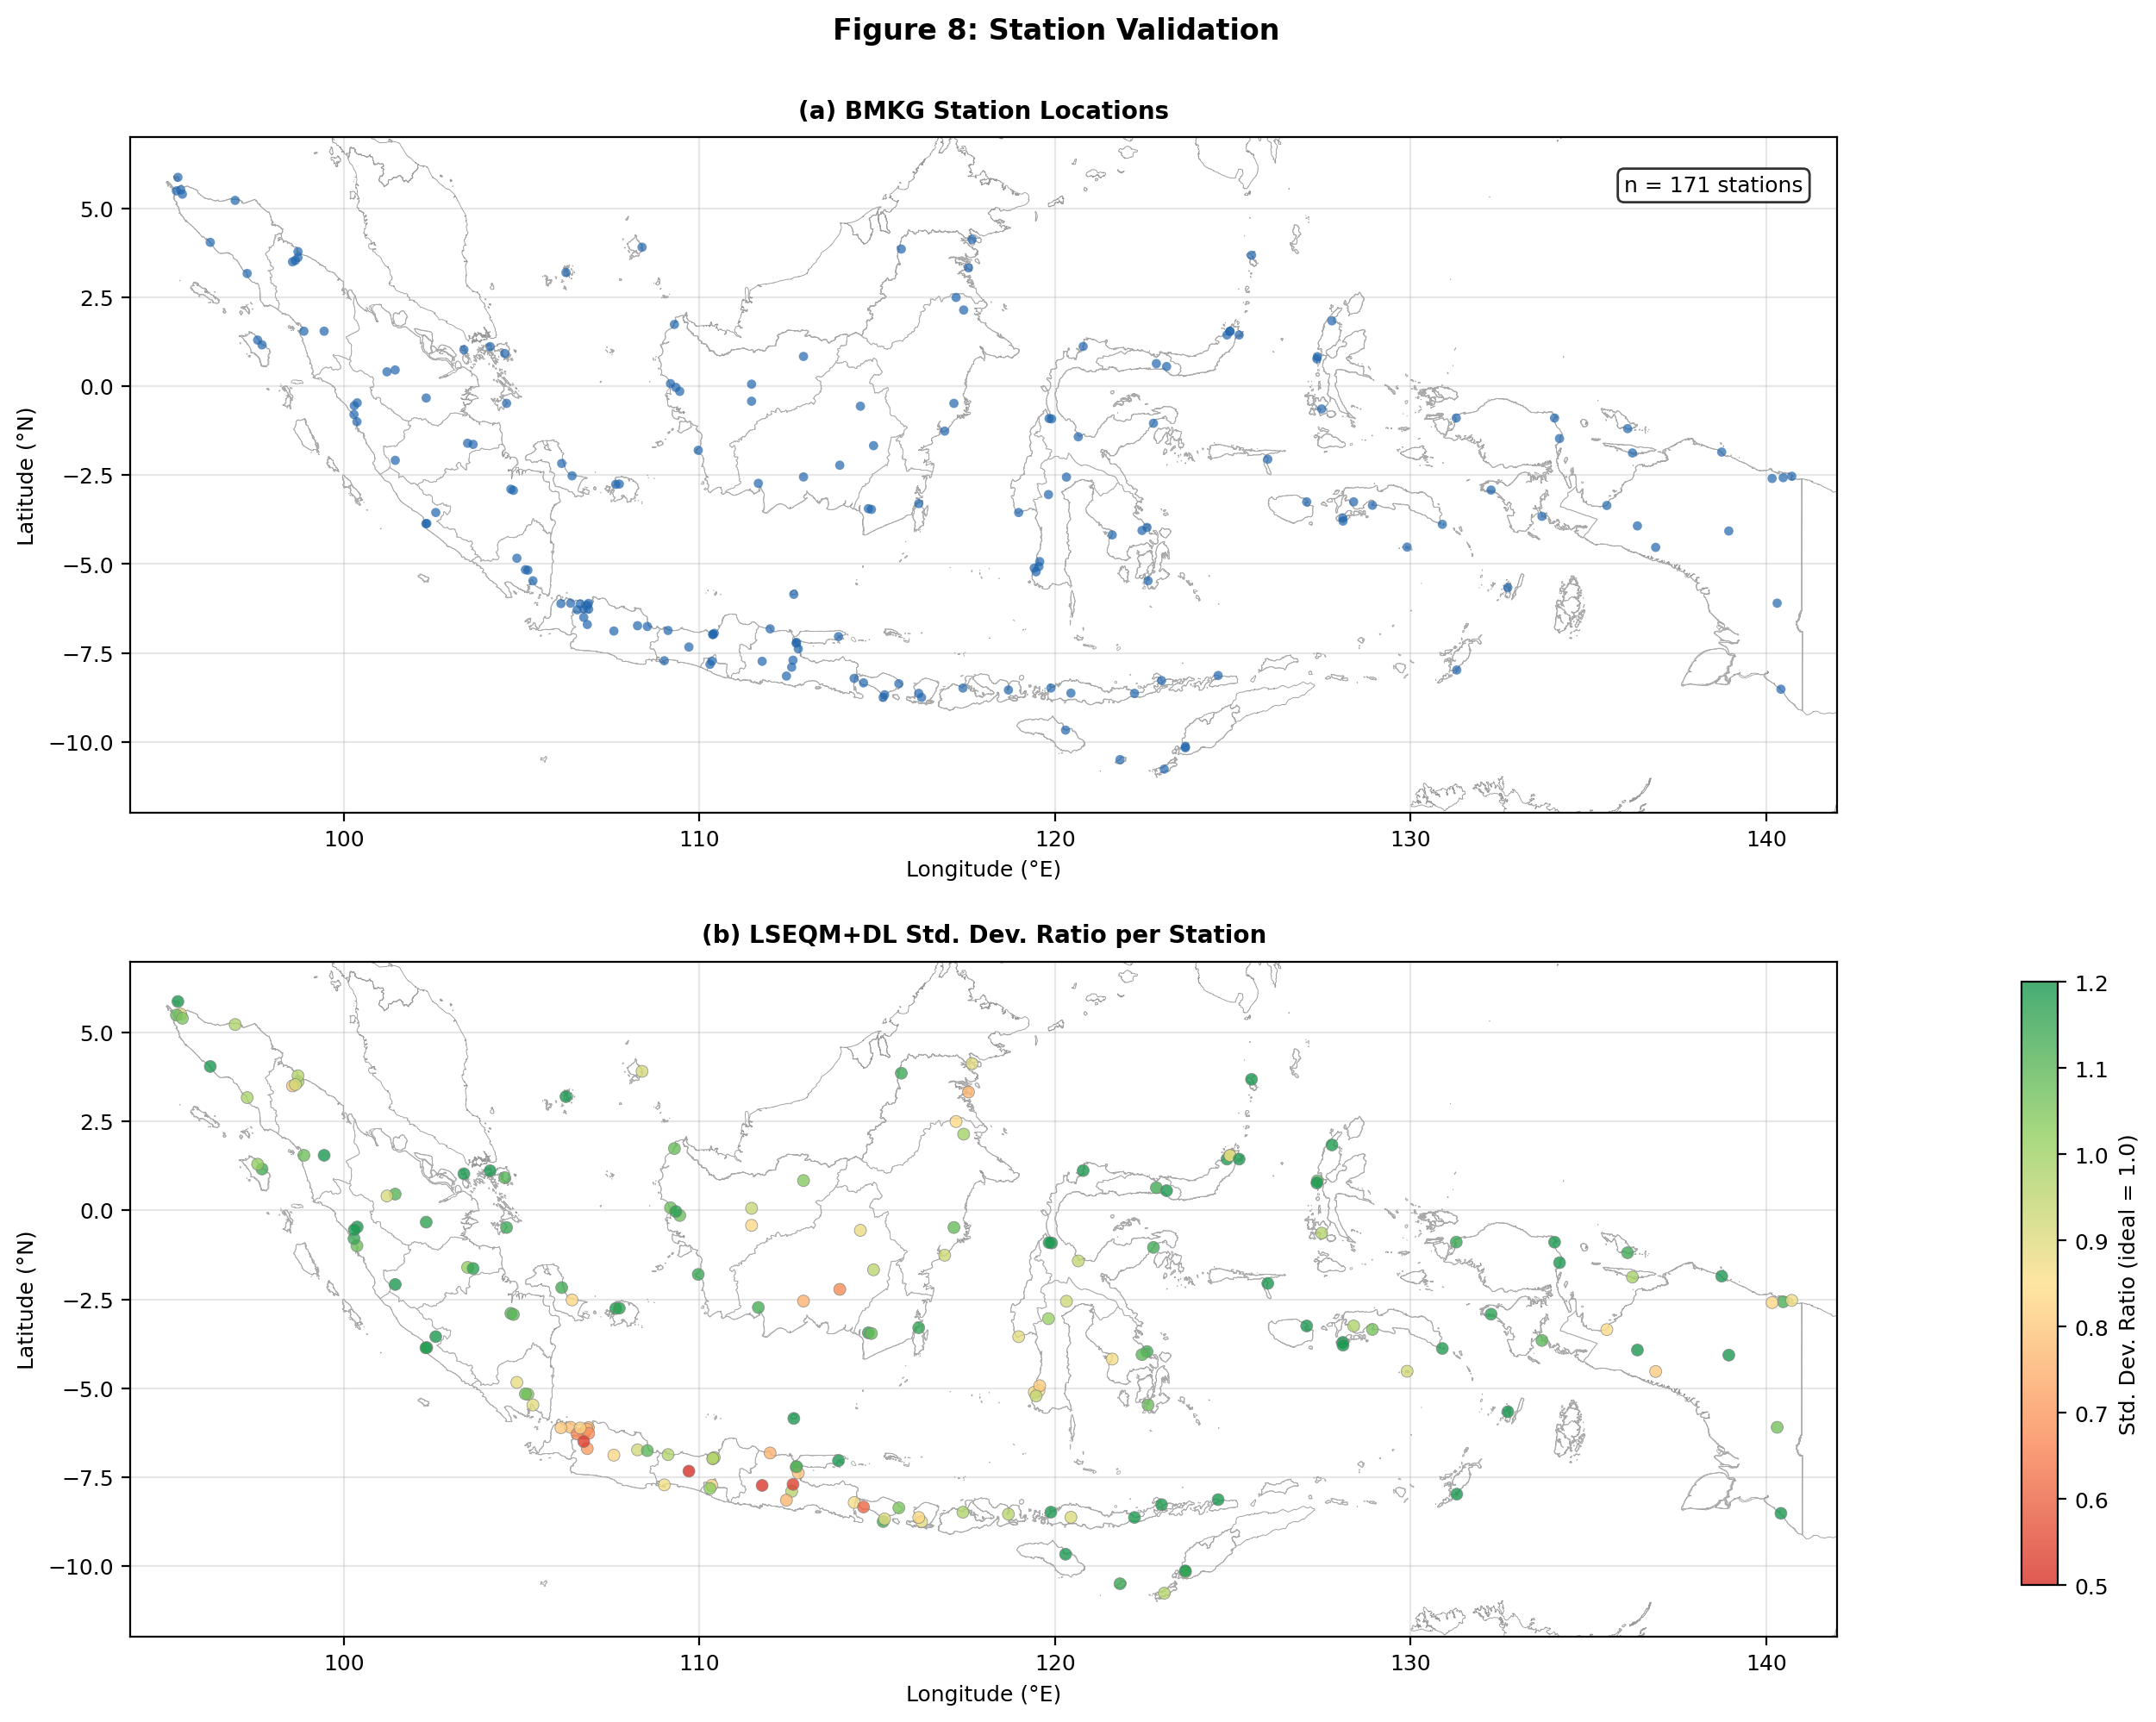
\includegraphics[width=\textwidth]{images/fig08_station_validation.png}
\caption{(a) Location of BMKG weather stations used for independent validation (\(n\) = 171). (b) Per-station standard deviation ratio (test/observed) for the LSEQM+DL product, averaged across all dekadal periods. Values near 1.0 (green) indicate good variability preservation; values below 0.7 (red) indicate underestimation of observed variability.}\label{fig8}
\end{figure}

Table 7 presents the station-level validation results organized by the
same three-pillar framework used for the domain-wide evaluation. The
station-level results provide the clearest evidence of the framework's
effectiveness, as the BMKG observations represent direct ground truth
uncontaminated by the interpolation uncertainties present in the gridded
CPC-UNI reference.

\textbf{Table 7.} Independent station validation organized by the three
design objectives of the hybrid framework. Values represent the median
across 171 BMKG stations and all 36 dekadal periods. Ratio metrics
express test/observed (target = 1.0). Bold indicates the value closest
to the target.

\begingroup\small
\begin{longtable}[]{@{}llllll@{}}
\toprule
Evaluation Objective & Metric & LS & LSEQM & LSEQM+DL & Target \\
\midrule
\endhead
\bottomrule
\endlastfoot
\textbf{Value Adjustment} & Relative Bias & $-$0.114 & \textbf{0.009}
& $-$0.006 & 0 \\
& Std. Dev. Ratio & 0.71 & 1.03 & \textbf{1.00} & 1.0 \\
\textbf{Distribution Alignment} & KS \(p\)-value (\%) & 0.01 &
\textbf{19.07} & \textbf{19.07} & 100 \\
& Wet-Day Freq. Ratio & 1.21 & \textbf{0.96} & \textbf{0.95} & 1.0 \\
& Mean Wet-Day Precip Ratio & 0.71 & \textbf{1.06} & \textbf{1.05} &
1.0 \\
\textbf{Extreme Preservation} & \(Q_{95}\) Ratio & 0.74 & \textbf{1.07}
& \textbf{1.05} & 1.0 \\
& \(Q_{99}\) Ratio & 0.71 & 1.05 & \textbf{1.01} & 1.0 \\
\textbf{Event Detection} & POD & \textbf{0.78} & 0.65 & 0.65 & 1.0 \\
& CSI & \textbf{0.53} & 0.49 & 0.49 & 1.0 \\
& FAR & 0.36 & \textbf{0.32} & \textbf{0.32} & 0 \\
\end{longtable}
\endgroup

The station-level results provide strong evidence for the framework's
effectiveness at independent ground truth locations. The most striking
changes occur in the LS-to-LSEQM transition. For value adjustment, the
standard deviation ratio improves from 0.71 to 1.03 --- meaning that LS
underestimates the observed precipitation variability by 29\%, while
LSEQM matches it within 3\%. The LSEQM+DL standard deviation ratio
reaches 1.00 (exact match to observed variability). For distribution
alignment, the wet-day frequency ratio moves from 1.21 to 0.96,
correcting a 21\% overestimation of wet-day occurrence to within 5\% of
observed. For extreme preservation, the \(Q_{99}\) ratio improves from
0.71 to 1.05, recovering the large extreme rainfall underestimation
present in the LS product; the full LSEQM+DL reaches \(Q_{99}\) = 1.01
(near perfect). The mean wet-day precipitation ratio improves from 0.71
to 1.06, indicating that the EQM adjustment corrects a systematic 29\%
underestimation of rainfall intensity on wet days to within 6\% of
observed values.

These improvements come at a measurable cost in event detection: POD
decreases from 0.78 (LS) to 0.65 (LSEQM), while FAR improves from 0.36
to 0.32. This trade-off is inherent to the dry-day frequency matching
\cite{ref11} (Section 3.3), which adjusts the marginal wet-day fraction to
match the CPC-UNI reference: some IMERG wet days that correspond to
genuine station-observed rainfall are reclassified as dry. However, the
net effect is that detected events are more reliable (lower FAR), and
the distributional properties of the corrected product are substantially
more accurate.

The LSEQM-to-LSEQM+DL transition shows targeted refinement at the
station level: the \(Q_{99}\) ratio moves from 1.05 to 1.01, and the
standard deviation ratio from 1.03 to 1.00 --- both approaching unity.
This confirms that the CNN refinement, while conservative by design,
provides measurable additional value for extreme event representation.

As with the gridded evaluation, temporal accuracy metrics at stations
show no improvement: Pearson correlation remains at approximately 0.24,
and RMSE increases from 15.9 (LS) to 18.2 mm/day (LSEQM+DL). This
confirms that the framework's value lies in statistical property
correction rather than temporal prediction skill, consistent with
Section 4.1.

To evaluate extreme event detection skill across a range of
precipitation intensities, the WMO-standard multi-threshold verification
\cite{ref24} was applied. Figure 9 presents the Probability of Detection,
Critical Success Index, and Equitable Threat Score as functions of
precipitation threshold (1, 5, 10, 20, 50, 100, and 150 mm/day).

\begin{figure}[H]
\centering
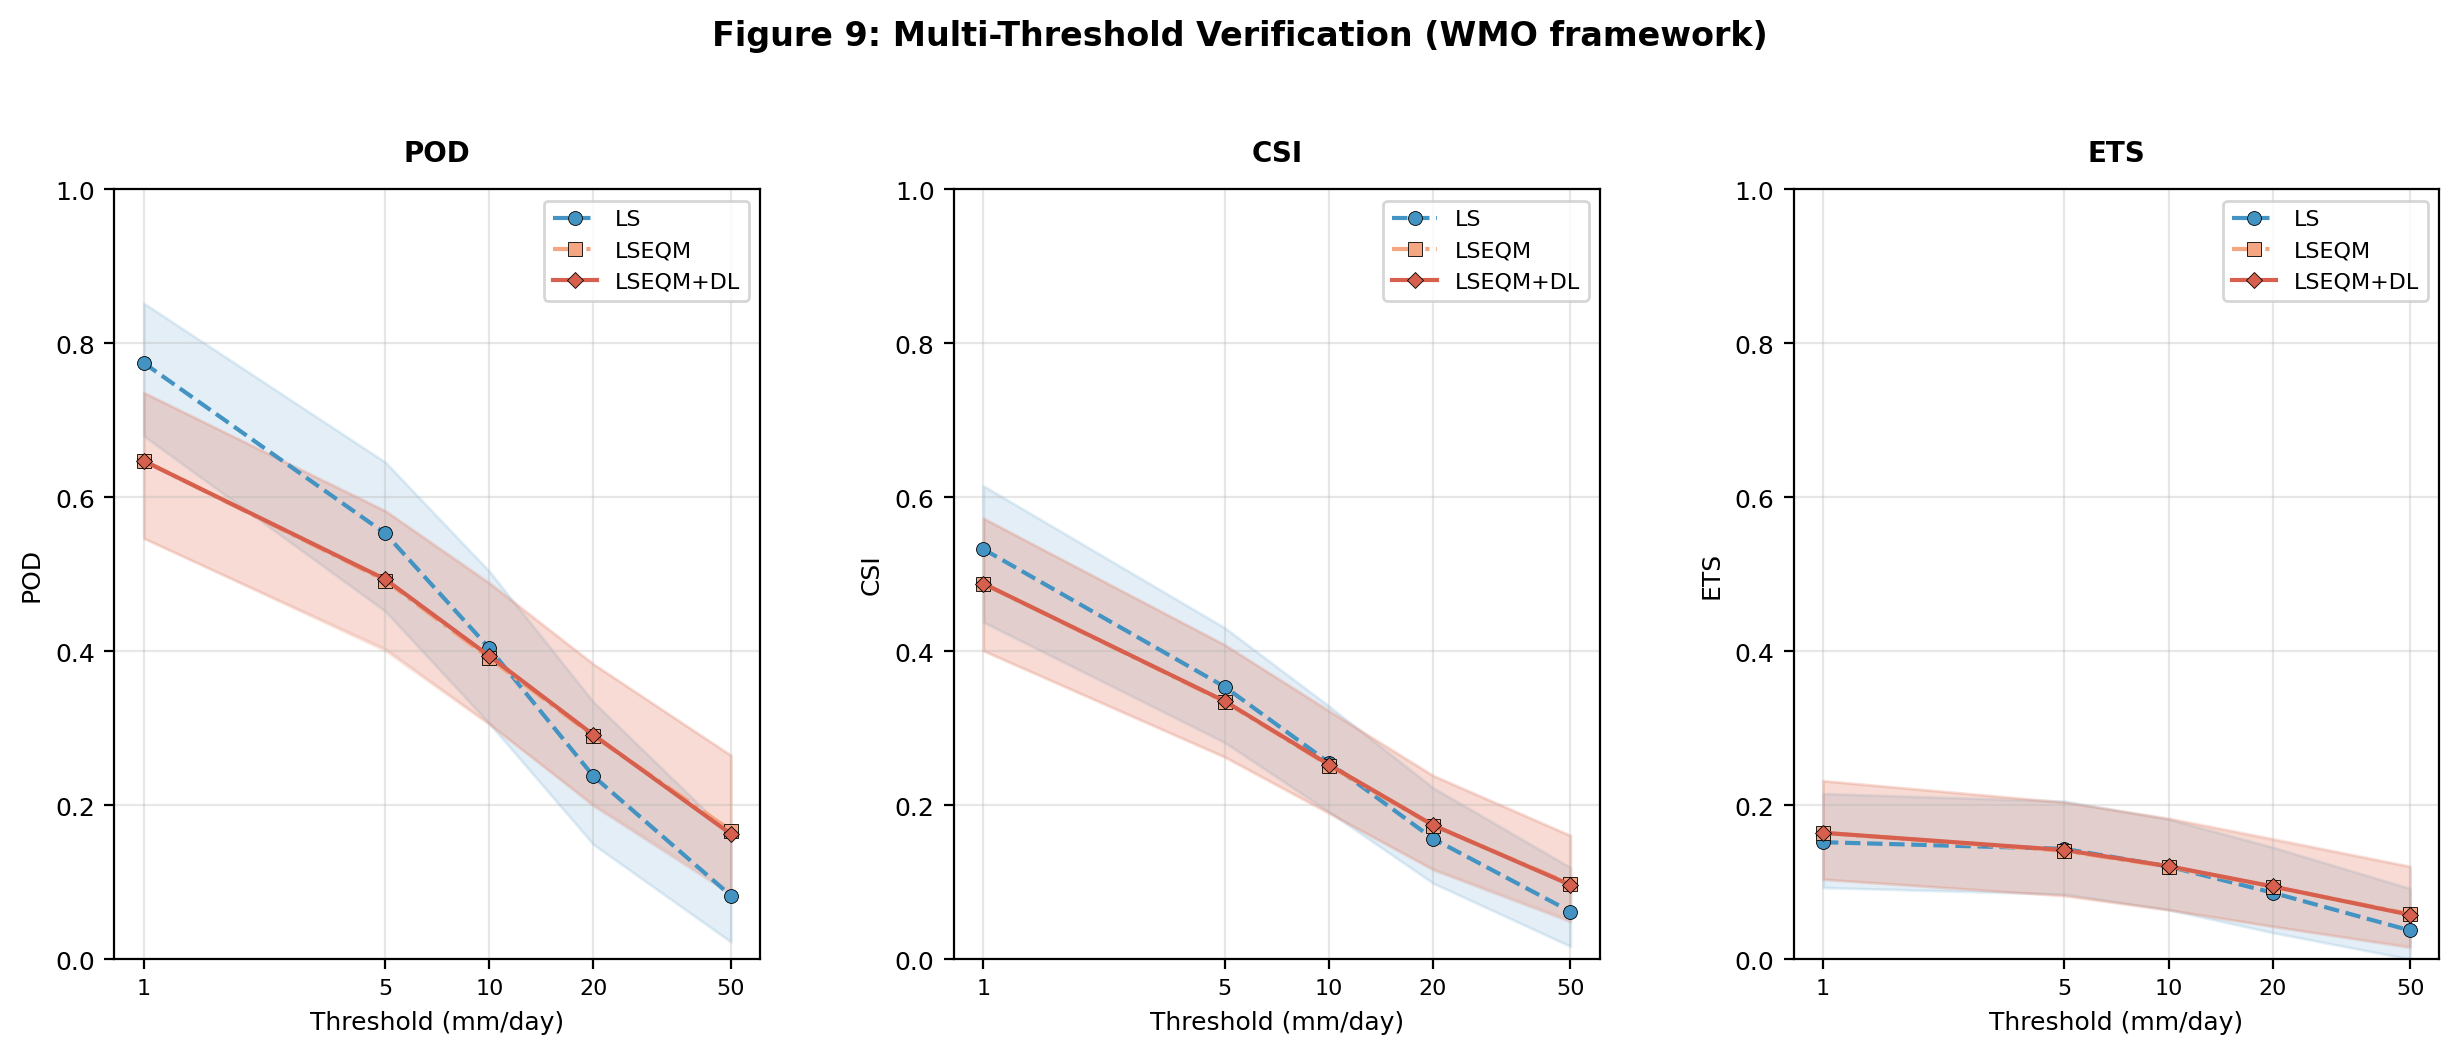
\includegraphics[width=\textwidth]{images/fig09_multi_threshold.png}
\caption{WMO multi-threshold verification: (a) Probability of Detection (POD), (b) Critical Success Index (CSI), and (c) Equitable Threat Score (ETS) as functions of precipitation threshold for LS (blue), LSEQM (orange), and LSEQM+DL (green). Lines show the median across all stations; shading indicates the interquartile range. Thresholds follow WMO classifications: 1 mm (measurable), 5 mm (light), 10 mm (moderate), 20 mm (moderate-heavy), 50 mm (heavy), 100 mm (very heavy), and 150 mm (extreme).}\label{fig9}
\end{figure}

All three methods show the expected decline in detection skill with
increasing threshold, as extreme events become rarer and more difficult
to reproduce. The LSEQM and LSEQM+DL curves are nearly indistinguishable
across all thresholds, reflecting the fact that the CNN refinement
adjusts precipitation magnitudes for extreme pixels but does not alter
wet/dry classification --- the contingency tables underlying POD, CSI,
and ETS are therefore essentially identical for both methods. At the 1
mm threshold, LS achieves the highest POD (0.77) and CSI (0.53), while
LSEQM+DL shows lower POD (0.65) but also lower FAR, reflecting the
dry-day frequency matching \cite{ref11} described in Section 3.3. However,
at thresholds above 20 mm/day, this pattern reverses: LSEQM and LSEQM+DL
maintain higher skill than LS. At the 50 mm threshold, the median CSI
for LSEQM+DL is 0.097, compared to 0.062 for LS, representing an
improvement of 56\%. At 100 mm (very heavy rainfall), the LSEQM+DL
product achieves a median POD of 0.065 and CSI of 0.042, compared to LS
values of 0.015 and 0.011 respectively, demonstrating that the GPD tail
adjustment substantially improves the detection of high-impact events.
The Equitable Threat Score, which accounts for random hits, shows a
similar pattern: at 50 mm, the ETS for LSEQM+DL (0.058) exceeds that of
LS (0.038), confirming that the improved extreme detection is not
attributable to increased frequency bias.

These station-level results provide the strongest validation evidence in
this study, as BMKG observations are entirely independent of the
correction procedure and represent direct ground truth measurements.

\subsection{Role of the Station Density Confidence
Mask}

The station density confidence mask was introduced to manage the spatial
heterogeneity of CPC-UNI reference quality by modulating the CNN
contribution based on gauge network density. To evaluate the
effectiveness of this mechanism, Figure 10a presents the confidence mask
itself, derived from BMKG station counts per CPC-UNI grid cell, and
Figure 10b examines the relationship between station density and CQI
improvement.

\begin{figure}[H]
\centering
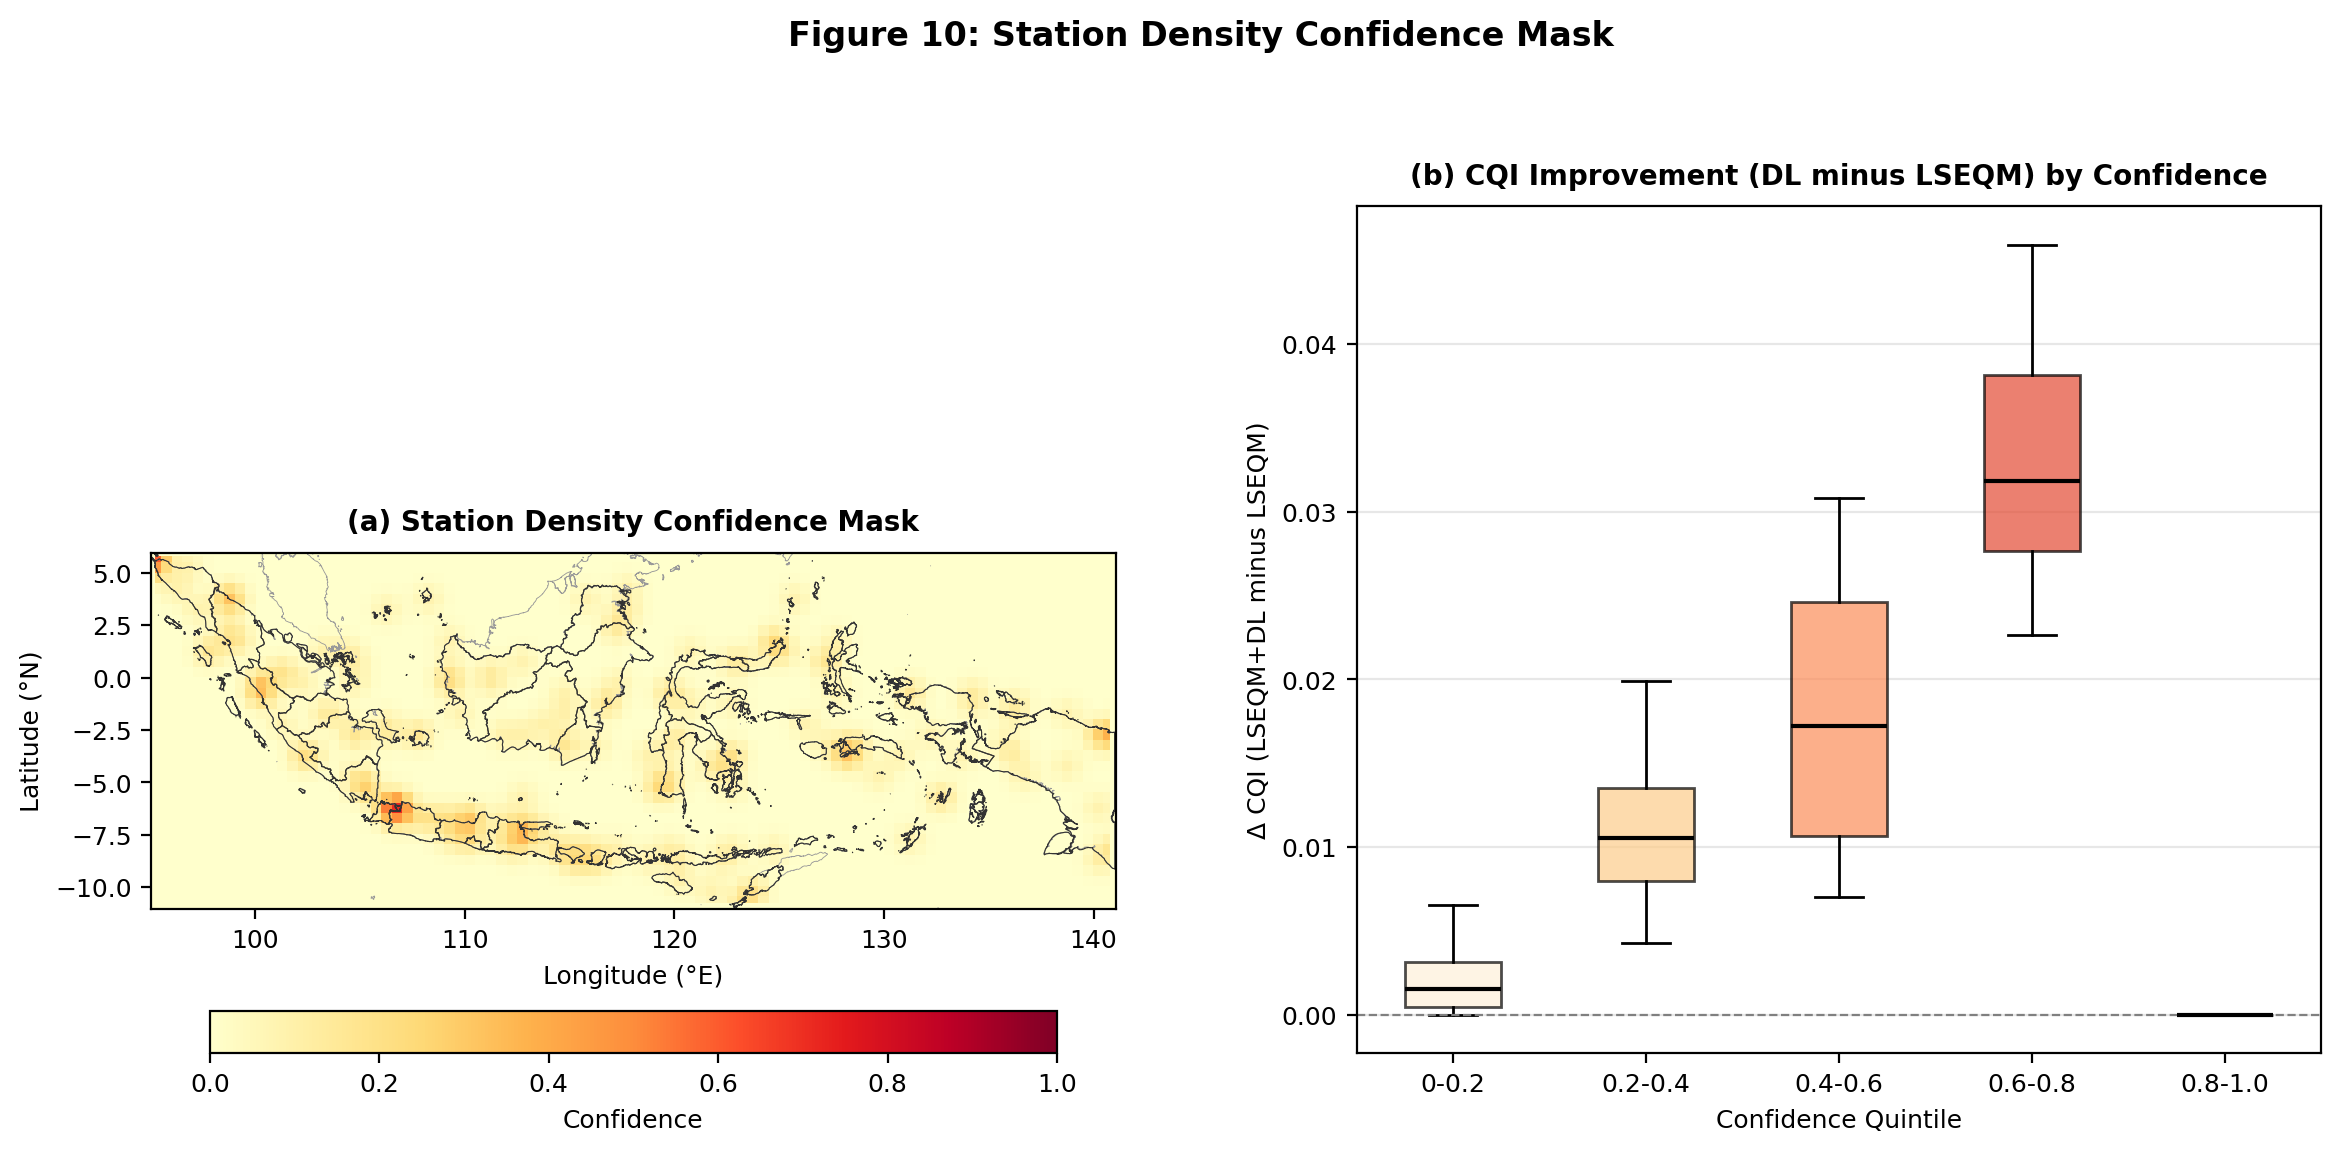
\includegraphics[width=\textwidth]{images/fig10_confidence_mask.png}
\caption{(a) Station density confidence mask \(C(x, y)\), ranging from 0 (no station coverage) to 1 (saturated coverage, \(\geq\) 3 stations per \(0.5^{\circ}\) cell). Gaussian smoothing (\(\sigma = 1\) grid cell) prevents sharp boundaries. (b) Relationship between confidence mask value and CQI improvement (LSEQM+DL minus LSEQM): box plots binned by confidence quintile.}\label{fig10}
\end{figure}

The confidence mask reveals the expected pattern: Java, Bali, and parts
of Sumatra have high confidence values (\(C > 0.7\)), while Papua,
Maluku, and oceanic boundary regions have near-zero confidence (25.8\%
of land pixels have \(C = 0\); median \(C = 0.002\)). The relationship
between confidence and CQI improvement (Figure 10b) demonstrates that
the mask operates as designed: the median \(\Delta\)CQI (LSEQM+DL minus
LSEQM) increases monotonically with confidence, from +0.002 at
\(C \in [0, 0.2)\) (\(n = 18{,}329\) pixels) to +0.011 at
\(C \in [0.2, 0.4)\) (\(n = 930\)), +0.017 at \(C \in [0.4, 0.6)\)
(\(n = 102\)), and +0.032 at \(C \in [0.6, 0.8)\) (\(n = 32\)). No
pixels reach \(C \geq 0.8\), reflecting the inherent sparsity of
Indonesia's gauge network. This monotonic relationship confirms that the
framework reverts to purely statistical corrections where the training
target is unreliable and concentrates CNN refinement where the reference
is well constrained.

This behavior has important practical implications. The confidence mask
provides users with a spatially explicit quality flag: regions with high
confidence values can be considered reliable for climate analysis and
risk assessment, while low-confidence regions require additional caution
or supplementary validation. For operational agencies such as BMKG, this
information supports decision-making about where the corrected product
can be used with confidence and where gauge-based assessments remain
necessary.

\subsection{Temporal Stability of
Corrections}\label{temporal-stability-of-corrections}

An important practical consideration for operational deployment is
whether the correction quality remains stable across the annual cycle or
varies systematically between wet and dry seasons. Figure 11 presents
monthly domain-median values of four key metrics --- standard deviation
ratio, RMSE, KS \(p\)-value, and CSI --- for all three correction
stages.

\begin{figure}[H]
\centering
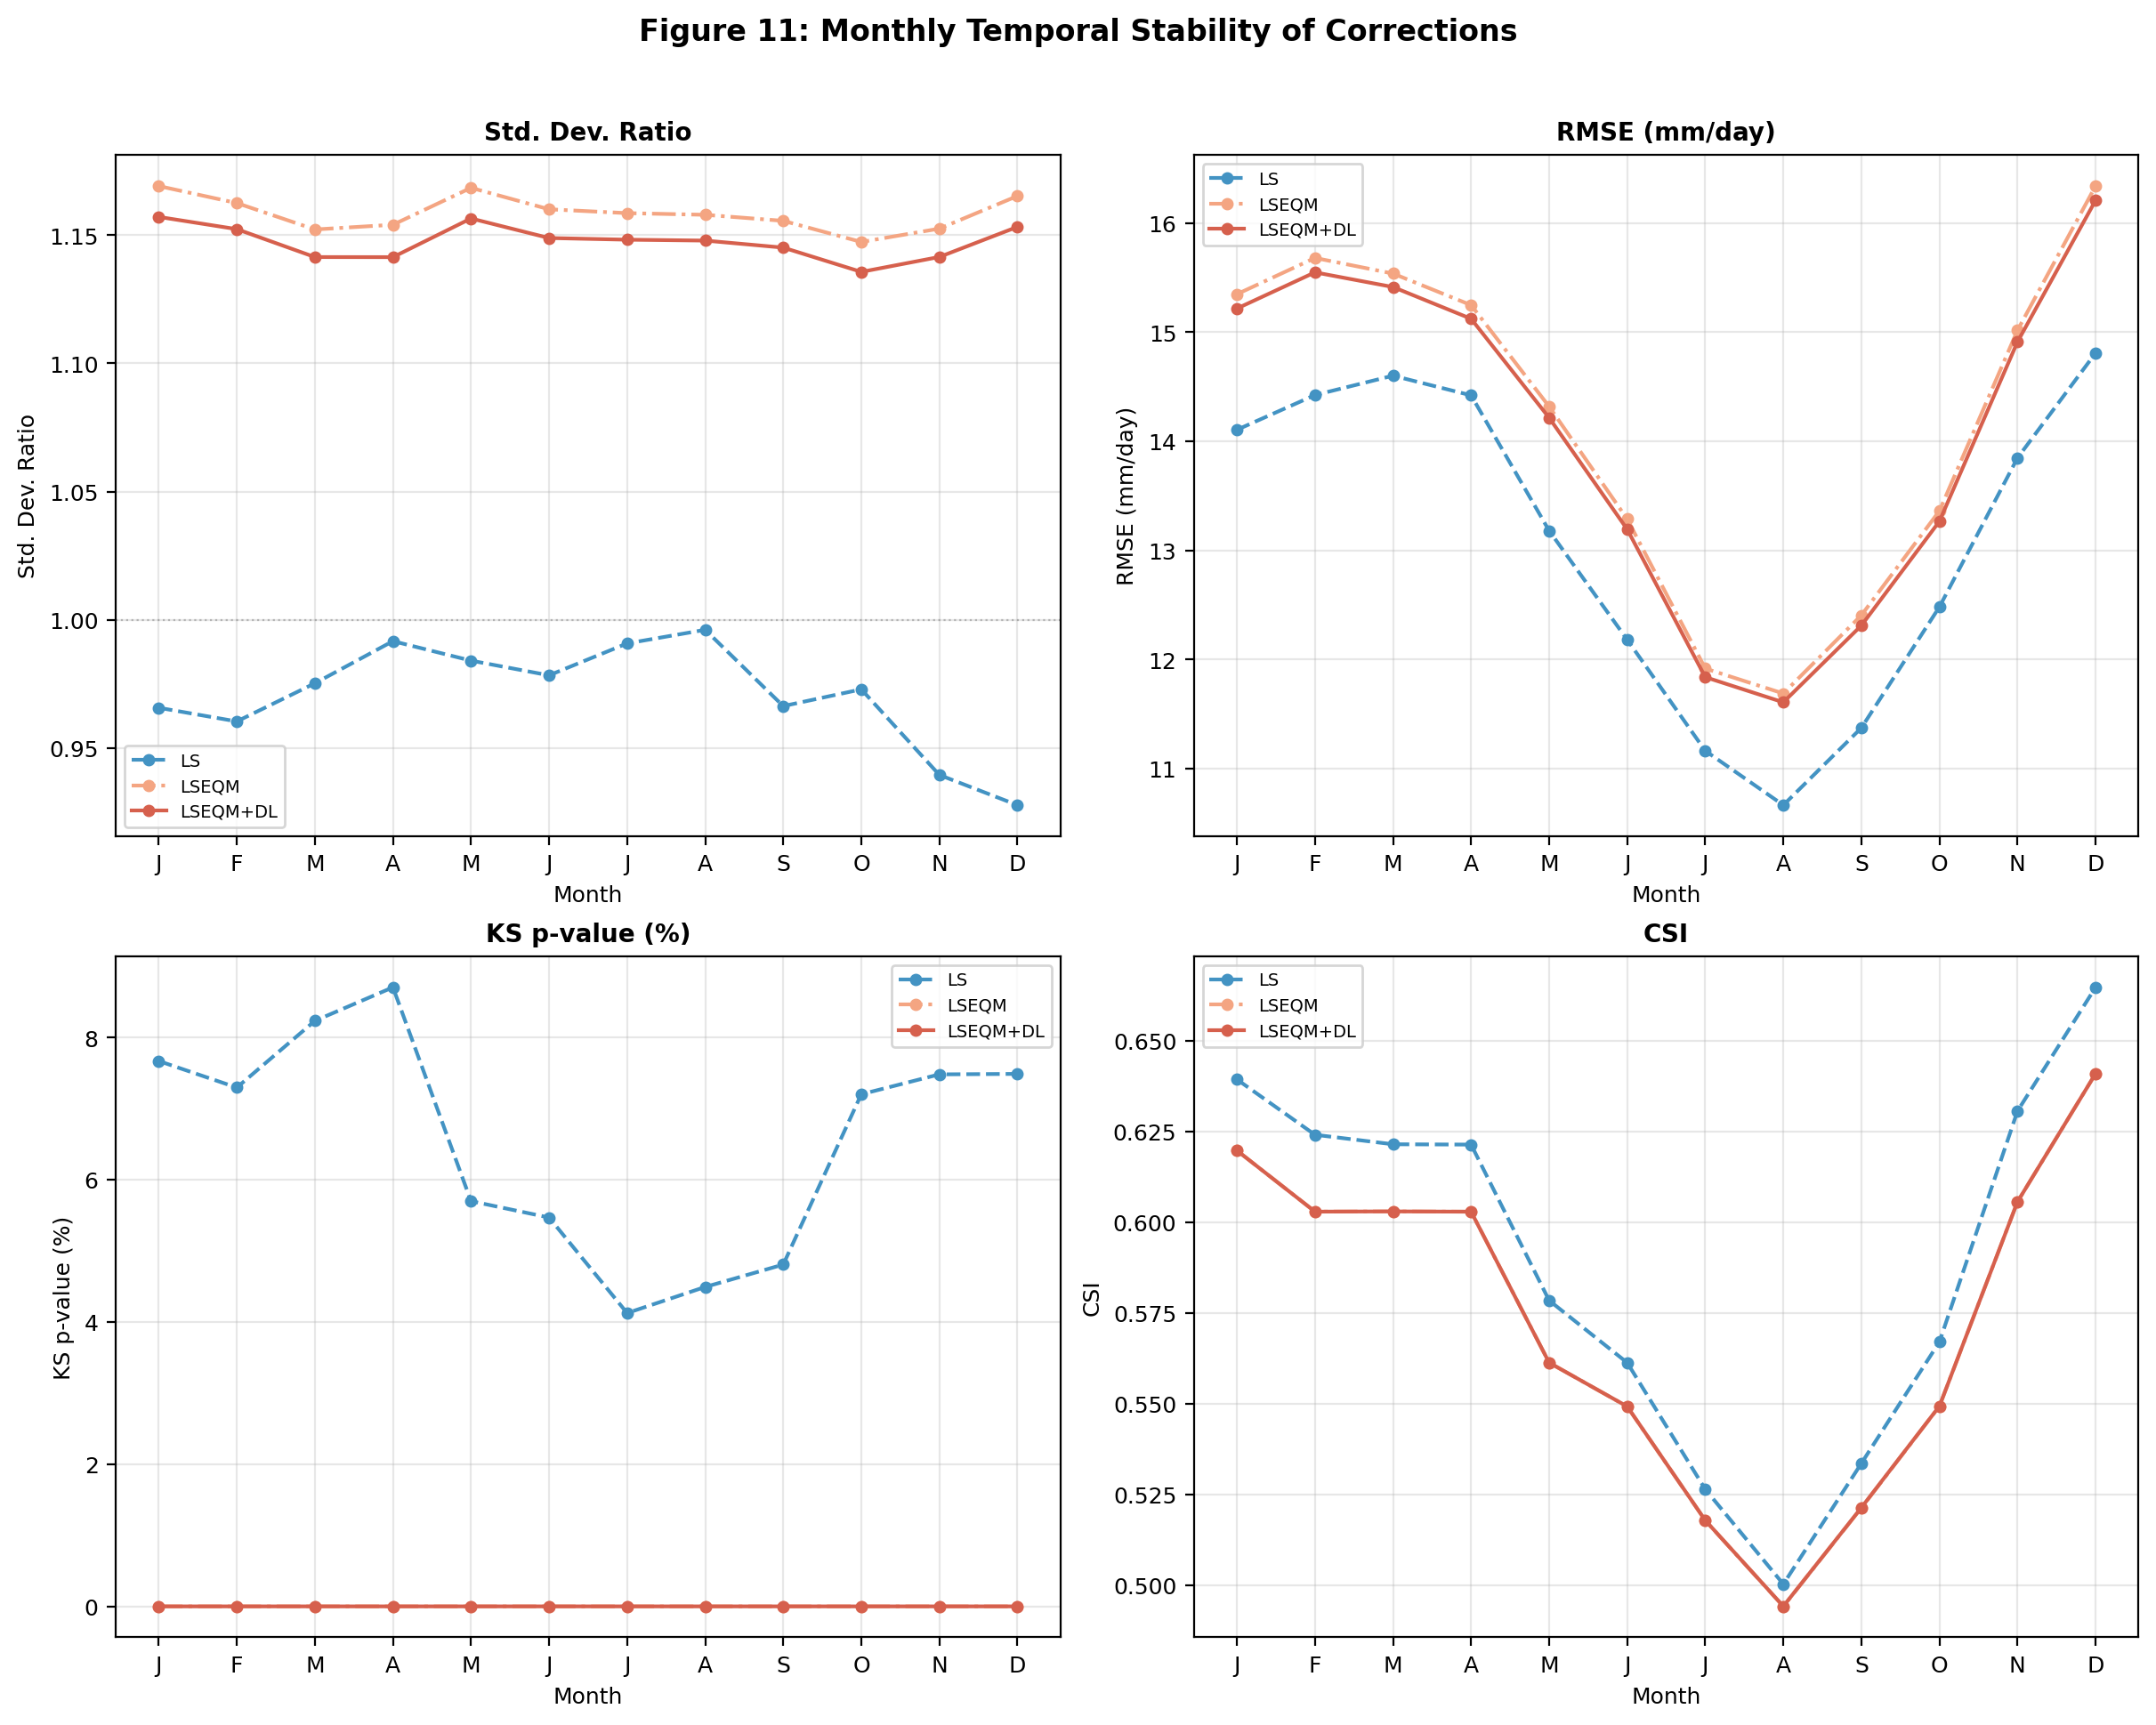
\includegraphics[width=\textwidth]{images/fig11_temporal_stability.png}
\caption{Monthly temporal stability of correction performance: (a) standard deviation ratio, (b) RMSE (mm/day), (c) KS \(p\)-value (\%), and (d) Critical Success Index (CSI). Lines show domain-median values for LS (blue), LSEQM (orange), and LSEQM+DL (green) across all 12 months. The seasonal cycle reflects the wet (October--March) and dry (April--September) monsoon regime.}\label{fig11}
\end{figure}

The standard deviation ratio (Figure 11a) shows that LSEQM and LSEQM+DL
maintain a consistently higher variability than LS across all months,
with values ranging from approximately 1.10 to 1.18 compared with
0.94--0.97 for LS. The relative ordering of methods is stable throughout
the year, indicating that the distributional correction does not
introduce seasonal artifacts. RMSE (Figure 11b) follows the expected
seasonal pattern, peaking during the wet season (December--March) when
precipitation intensities are highest and declining during the dry
season (June--September). LSEQM and LSEQM+DL show moderately higher RMSE
than LS, consistent with the wider corrected distribution discussed in
Section 4.1.

The KS \(p\)-value (Figure 11c) reveals a seasonal pattern for LS, with
higher values during the dry season when both satellite and reference
distributions are more similar due to reduced precipitation. LSEQM and
LSEQM+DL maintain near-zero KS \(p\)-values throughout the year,
reflecting the intentional distributional shift. CSI (Figure 11d) shows
a modest seasonal cycle for all methods, with slightly lower values
during the dry season transition months (April--May). The LS-to-LSEQM
gap in CSI (approximately 0.02--0.03) is consistent across months,
confirming that the POD trade-off discussed in Section 4.5 is not
seasonally concentrated.

\subsection{Discussion}\label{discussion}

\paragraph{Synthesis of the Sequential Hybrid
Approach}

The results presented in Sections 4.1 through 4.6 demonstrate that the
sequential LSEQM+DL framework delivers measurable improvements across
its three design objectives: adjusting values, aligning distributions,
and preserving extremes. Each processing stage addresses a distinct
aspect of satellite precipitation bias. Linear Scaling corrects the
first moment (mean bias). EQM aligns the full marginal distribution,
bringing the wet-day frequency, variability, and moderate percentiles
into agreement with the reference. GPD tail adjustment preserves extreme
event magnitudes that standard EQM attenuates due to limited sampling in
the upper tail. The CNN refinement provides spatial consistency by
learning residual patterns from the corrected fields. The
dual-resolution fitting strategy, which estimates CPC-UNI distribution
parameters at the native \(0.5^{\circ}\) grid and interpolates them
smoothly to the \(0.1^{\circ}\) IMERG grid (Section 3.3), produces
spatially continuous correction fields consistent with the BCSD
principle \cite{ref23}.

The clearest demonstration of this sequential design comes from the
independent station validation (Table 7), where each pillar shows
substantial improvement from LS to LSEQM: the standard deviation ratio
improves from 0.71 to 1.03 (and to 1.00 under LSEQM+DL), the \(Q_{99}\)
ratio from 0.71 to 1.05 (1.01 under LSEQM+DL), and the wet-day frequency
bias decreases from 21\% to 5\%. These improvements at independent
ground truth locations confirm that the framework addresses genuine
precipitation biases rather than merely fitting the training reference.

An equally important finding is that distributional bias correction does
not improve --- and is not designed to improve --- temporal prediction
skill at the pixel level. Correlation, RMSE, and NSE remain largely
unchanged across correction stages (Section 4.1), consistent with the
theoretical understanding that quantile mapping adjusts marginal
distributions without modifying the temporal ordering of values
\cite{ref34}. This distinction is critical for users: the corrected product
should be interpreted as having improved statistical properties (bias,
variability, distribution shape, extreme magnitudes) rather than
improved day-to-day prediction accuracy. Applications that require
temporally accurate fields, such as real-time flood forecasting, should
use the corrected product in combination with temporal downscaling or
ensemble methods.

This sequential design offers advantages over both purely statistical
and purely DL approaches. Single-method statistical corrections can
align distributions but may not capture complex spatial patterns driven
by topography and atmospheric processes \cite{ref8,ref44}. Standalone DL
approaches can learn spatial relationships but risk introducing
physically implausible values if not adequately constrained \cite{ref9,ref12}.
By positioning the CNN as a refinement step after statistical
correction, the DL component operates on partially corrected input from
the same statistical domain used during training, avoiding the domain
shift problem that can degrade purely DL methods.

The alpha-blending strategy further constrains the DL contribution by
design: the base weight of 0.70 assigns dominant influence to the
statistical correction, while the CNN provides targeted refinement for
extreme pixels only. This conservative integration reflects the
principle that statistical methods with established theoretical
foundations should anchor the correction, with machine learning serving
as a complementary tool rather than a replacement.

It should also be noted that IMERG-L is known to over-detect light and
drizzle-class precipitation over the tropical oceans and coastal zones,
a characteristic consistently reported in independent evaluations
\cite{ref31,ref32}. The R1 contribution identified in Section 4.1.1 is
consistent with this well-documented light-rain over-detection. Because
LSEQM operates pixel-wise on marginal distributions, it partially
flattens but does not eliminate this signature, which is revisited in
Section 4.8.5.

\paragraph{Extreme Event
Representation}\label{extreme-event-representation}

The preservation of extreme precipitation events emerged as a key
strength of the framework. The GPD tail adjustment at the 80th
percentile threshold addresses a well-documented limitation of standard
EQM: the tendency to attenuate extreme values due to insufficient
sampling in the upper tail of the empirical distribution \cite{ref11}. By
modeling exceedances explicitly and employing K-fold cross-validation
for parameter estimation, the GPD stage provides stable extreme quantile
corrections even in regions with limited observational samples.

The WMO multi-threshold verification (Figure 9) provides strong
quantitative evidence, as it evaluates detection skill across the full
precipitation intensity spectrum using operationally defined thresholds.
The maintained skill at thresholds above 50 mm/day is critical for
applications in flood early warning and urban drainage design, where
accurate representation of heavy and extreme rainfall directly impacts
risk assessment and emergency response planning.

\paragraph{Practical Implications of the Confidence
Mask}

The station density confidence mask addresses a challenge common to all
bias correction methods that rely on gridded gauge products: the spatial
heterogeneity of reference data quality. As demonstrated in Section 4.6,
the mask modulates the DL influence based on the density of contributing
stations, preventing CNN artifacts in poorly observed regions.

A practical advantage of this design is its transferability. The mask
adapts automatically to any station network, requiring no manual tuning
of regional parameters. For regions with denser networks (e.g., parts of
India, Japan), the mask would permit greater DL influence, while regions
with sparser coverage (e.g., Central Africa, the Amazon basin) would
receive predominantly statistical corrections. The mask also serves as a
spatially explicit quality indicator for end users, supporting
operational decisions about where the corrected product can be applied
for climate analysis, hydrological modeling, or risk assessment.

\subsubsection{Limitations}\label{limitations}

Several limitations should be acknowledged. First, the bias correction
is performed separately for each dekadal period, pooling daily values
across years. This design preserves seasonal characteristics and
provides adequate sample sizes for distribution fitting, but does not
explicitly model temporal autocorrelation within each dekad or
inter-annual trends in precipitation patterns.

Second, the CPC-UNI reference product is available at \(0.5^{\circ}\)
spatial resolution, considerably coarser than the \(0.1^{\circ}\) IMERG
grid. The dual-resolution fitting strategy (Section 3.3) produces
spatially smooth correction fields by interpolating fitted parameters,
but the correction still targets the spatial scales resolved by CPC-UNI
rather than the finer scales present in IMERG. Bilinear interpolation of
parameters does not introduce sub-grid variability. Consequently, the
framework corrects the coarse-scale distributional properties of the
precipitation field without adding fine-scale detail in regions of
complex topography.

Third, the CNN architecture employs a Flatten-Dense bottleneck that
compresses spatial information into a one-dimensional representation
before reconstruction. This relatively simple architecture was selected
deliberately: because the CNN operates as a refinement step on
already-corrected fields rather than as the primary correction, a
lightweight model reduces overfitting risk and training cost.
Nevertheless, fully convolutional architectures (e.g., U-Net) that
preserve spatial resolution throughout the network could improve
performance and would be worth exploring in future work.

Fourth, this study demonstrates the framework over a single domain
(Indonesia) and a single temporal period (2001--2025 for IMERG Late Run
and CPC-UNI). While the methodology relies on globally available
datasets (IMERG and CPC-UNI) and employs transferable statistical
methods, the optimal GPD threshold, CNN hyperparameters, and
alpha-blending weight may require recalibration for different climate
regimes \cite{ref44,ref45}. Performance varies between the wet season
(October--March) and dry season (April--September), as detailed in
Section 4.7.

Fifth, the evaluation uses the same temporal period for both correction
and assessment. A strict temporal hold-out (e.g., training on 2001--2020
and evaluating on 2021--2025) would provide a more rigorous assessment
of generalization, though at the cost of reducing the training sample
from approximately 250 to 200 daily values per dekad, which may
compromise GPD parameter stability. The use of independent validation
against BMKG stations (Section 4.5) partially mitigates this concern.

Sixth, the alpha-blending weight (\(\alpha = 0.70\)) and GPD threshold
percentile (80th) were selected based on domain expertise rather than
formal optimization. A sensitivity analysis varying these parameters
could identify performance trade-offs and inform region-specific
calibration. Similarly, the QA framework component weights (basic
statistical quality: 0.35, distribution quality: 0.35, temporal quality:
0.30) represent a subjective but informed partitioning of quality
dimensions; alternative weightings could shift the CQI values and
categorical classifications, though the relative ranking of correction
methods is expected to be robust to reasonable weight perturbations.

\paragraph{Residual Bias
Attribution}\label{residual-bias-attribution}

After LSEQM correction, IMERG-L exhibits a residual positive bias of
approximately \(+8\%\) against CPC-UNI over Indonesia during peak
monsoon (January dekad 1, land pixels only), compared with \(+15.5\%\)
for the raw IMERG-L product. This residual persists across daily and
dekadal evaluation framings and across alternative tail-handling
configurations (parametric GPD, empirical tail, frequency-matched
drizzle suppression), indicating a structural rather than methodological
origin.

Two factors inherent to the CPC-UNI reference explain the floor. First,
CPC-UNI systematically undercatches convective precipitation over
sparsely gauged mountainous terrain in the tropics, a well-documented
limitation of gauge-based interpolation products \cite{ref36,ref37}. Second,
the \(0.5^{\circ}\) gauge analysis cannot resolve sub-grid heterogeneity
that is physically present in the \(0.1^{\circ}\) satellite retrieval,
so a portion of the IMERG wet signal that is locally correct at
\(0.1^{\circ}\) is unrecoverable at the CPC-UNI resolution regardless of
statistical treatment.

The magnitude of the residual is consistent with published independent
evaluations of IMERG-L over the Maritime Continent. Several studies
using diverse reference datasets \cite{ref31,ref32,ref33,ref38,ref39,ref47} report
satellite wet biases in the range of \(+10\%\) to \(+25\%\) during the
wet season for this region. The \(+8\%\) residual reported here after
LSEQM therefore falls at the lower end of the published wet-season
range.

The per-pixel R1/R2/R3 decomposition (Section 4.1.1) further shows that
the residual is conditional in nature: IMERG is too wet on CPC
light-rain days (R1 \(\approx +31\) pp) and simultaneously too dry on
CPC moderate-to-extreme days (R2 \(\approx -21\) pp, R3 \(\approx -2.6\)
pp), and these sign-opposite errors partially cancel in the domain
summary. Because marginal quantile mapping adjusts each pixel's CDF
without reassigning values to days, a conditional mismatch of this form
cannot be removed by LSEQM or by any univariate bias correction method
by construction \cite{ref34,ref11}. It reflects a mismatch in \emph{which days
are heavy where} between IMERG and the gauge analysis, not a mismatch in
the marginal distribution of daily intensities.

Taken together, these observations support interpreting the post-LSEQM
residual as reference-side uncertainty rather than correction
deficiency. The station-level validation against BMKG observations
(Section 4.5) provides the independent ground-truth perspective required
to resolve this interpretation, and shows that LSEQM moves the standard
deviation ratio, wet-day frequency, and \(Q_{99}\) toward the gauge
observations even where it moves away from the gridded CPC-UNI
reference.

\subsubsection{Future Directions}\label{future-directions}

Several extensions of this work merit investigation. Replacing the Dense
reconstruction layer with a fully convolutional architecture (e.g.,
U-Net) could improve the spatial fidelity of the CNN refinement
\cite{ref40,ref41}, particularly over regions with sharp topographic gradients.
Incorporating additional predictive features, such as elevation, land
cover type, and distance to coast, as auxiliary CNN input channels could
provide the model with physically meaningful spatial context beyond the
precipitation field alone.

Extending the framework to other satellite precipitation products (e.g.,
CHIRPS, GSMaP, MSWEP \cite{ref42}) and other correction-reference pairings
would test the generalizability of the sequential approach. Application
to other tropical and subtropical regions with sparse gauge networks,
such as Sub-Saharan Africa and the Amazon basin, would directly assess
the transferability claim.

At the temporal scale, extending the framework from dekadal to pentad
(5-day) or individual daily corrections would increase the temporal
specificity of the bias correction, though at the cost of reduced sample
sizes per fitting window. Adaptive window sizing, where the pooling
period is adjusted based on data availability, could balance temporal
specificity against statistical robustness.

A formal sensitivity analysis of the alpha-blending weight and GPD
threshold percentile, potentially using cross-validated grid search
\cite{ref43}, would establish whether the current parameter choices are
stable across different climate regimes or require region-specific
tuning. Similarly, a strict temporal hold-out experiment would
strengthen the generalization claims, and is planned as part of the
operational deployment of this framework.

Finally, the framework could be extended to address additional
precipitation characteristics beyond daily accumulations, such as
sub-daily intensity, the diurnal cycle, or multi-day event persistence,
which are important for hydrological applications but are not explicitly
targeted by the current dekad-based correction design.

\section{Conclusions}\label{conclusions}

This study developed and evaluated a hybrid bias correction framework
(LSEQM+DL) for daily satellite precipitation that sequentially applies
Linear Scaling, Empirical Quantile Mapping with Generalized Pareto
Distribution (GPD) tail adjustment, and Convolutional Neural Network
(CNN) refinement. Applied to IMERG Late Run daily precipitation over
Indonesia (2001--2025) and evaluated against CPC-UNI and 171 independent
BMKG station observations, the framework yields four principal findings,
organized around its three design objectives: adjusting values, aligning
distributions, and preserving extremes.

First, the sequential design delivers measurable improvements across all
three objectives. At independent BMKG station locations, the standard
deviation ratio improves from 0.71 (LS) to 1.03 (LSEQM) and 1.00
(LSEQM+DL), the wet-day frequency bias decreases from 21\% to 5\%, and
the \(Q_{99}\) ratio improves from 0.71 to 1.05 (LSEQM) and 1.01
(LSEQM+DL), recovering the extreme rainfall underestimation present in
the LS product. These improvements come at a measurable cost in event
detection (POD decreases from 0.78 to 0.65), a trade-off inherent to the
dry-day frequency matching \cite{ref11} that is partially offset by improved
FAR (0.36 to 0.32). Each correction stage targets a distinct bias
dimension: LS adjusts the mean, EQM aligns the distribution, and GPD
preserves the extremes.

Second, the framework honestly operates within the known limitations of
distributional bias correction: pixel-level temporal accuracy
(correlation, RMSE, NSE) remains largely unchanged across correction
stages, consistent with the theoretical understanding that quantile
mapping adjusts marginal distributions without modifying temporal
sequencing \cite{ref34}. This distinction is important for users: the
corrected product has improved statistical properties (bias,
variability, distribution shape, extreme magnitudes) but not improved
day-to-day prediction accuracy.

Third, independent validation against 171 BMKG stations strengthens
confidence that the improvements reflect genuine enhancement of the
precipitation signal rather than overfitting to the CPC-UNI training
reference. The domain-wide CQI decreases from 0.541 (LS) to 0.508
(LSEQM+DL), driven by the POD trade-off in the composite index; however,
the station-level validation confirms that the distributional
corrections move the product toward independent ground truth. The WMO
multi-threshold verification further demonstrates that at thresholds
above 20 mm/day, LSEQM+DL maintains higher detection skill than LS, with
the CSI at 50 mm improving by 56\%.

Fourth, the station density confidence mask provides a practical
mechanism for managing reference dataset uncertainty. By modulating the
CNN influence based on gauge network density, the mask prevents DL
artifacts in station-sparse regions while allowing CNN refinement where
the reference is well constrained. The mask also serves as a spatially
explicit quality flag for end users.

Several limitations warrant consideration, including the absence of a
strict temporal hold-out, the use of a relatively simple CNN
architecture, and the reliance on fixed values for the blending weight
and GPD threshold that were not formally optimized. These choices were
guided by practical constraints of limited training samples per dekad
($\sim$230 daily values) and the design priority of maintaining
physical plausibility over maximizing statistical fit. Future work
should address these limitations through sensitivity analysis,
alternative architectures such as U-Net, and application to additional
tropical regions to test transferability.

The framework relies on globally available datasets (IMERG and CPC-UNI)
and employs transferable statistical-distributional methods, making it
applicable to other regions with sparse gauge networks. The modular
implementation supports integration into operational precipitation
monitoring workflows where climatologically unbiased daily estimates are
needed for hydrological modeling, agricultural planning, and climate
risk assessment.

%%%%%%%%%%%%%%%%%%%%%%%%%%%%%%%%%%%%%%%%%%


\begin{thebibliography}{47}


\bibitem{ref1} Hou, A.Y., Kakar, R.K., Neeck, S., Azarbarzin, A.A., Kummerow,
C.D., Kojima, M., Oki, R., Nakamura, K. and Iguchi, T. (2014). The
Global Precipitation Measurement Mission. \emph{Bull. Amer. Meteor.
Soc.}, 95(5), 701-722. DOI: 10.1175/BAMS-D-13-00164.1

\bibitem{ref2} Huffman, G.J., Bolvin, D.T., Braithwaite, D., Hsu, K.-L., Joyce,
R.J., Kidd, C., Nelkin, E.J., Sorooshian, S., Stocker, E.F., Tan, J.,
Wolff, D.B. and Xie, P. (2020). Integrated Multi-satellitE Retrievals
for the Global Precipitation Measurement (GPM) Mission (IMERG).
\emph{Satellite Precipitation Measurement}, Adv. Global Change Res., 67,
343-353. DOI: 10.1007/978-3-030-24568-9\_19

\bibitem{ref3} Maggioni, V., Meyers, P.C. and Robinson, M.D.~(2016). A Review
of Merged High-Resolution Satellite Precipitation Product Accuracy
during the Tropical Rainfall Measuring Mission (TRMM) Era. \emph{J.
Hydrometeor.}, 17(4), 1101-1117. DOI: 10.1175/JHM-D-15-0190.1

\bibitem{ref4} Teutschbein, C. and Seibert, J. (2012). Bias correction of
regional climate model simulations for hydrological climate-change
impact studies: Review and evaluation of different methods. \emph{J.
Hydrol.}, 456-457, 12-29. DOI: 10.1016/j.jhydrol.2012.05.052

\bibitem{ref5} Gudmundsson, L., Bremnes, J.B., Haugen, J.E. and Engen-Skaugen,
T. (2012). Technical Note: Downscaling RCM precipitation to the station
scale using statistical transformations -- a comparison of methods.
\emph{Hydrol. Earth Syst. Sci.}, 16, 3383-3390. DOI:
10.5194/hess-16-3383-2012

\bibitem{ref6} Themesssl, M.J., Gobiet, A. and Heinrich, G. (2012).
Empirical-statistical downscaling and error correction of regional
climate models and its impact on the climate change signal.
\emph{Climatic Change}, 112, 449-468. DOI: 10.1007/s10584-011-0224-4

\bibitem{ref7} Coles, S. (2001). \emph{An Introduction to Statistical Modeling
of Extreme Values}. Springer Series in Statistics. DOI:
10.1007/978-1-4471-3675-0

\bibitem{ref8} Maraun, D. (2016). Bias Correcting Climate Change Simulations --
a Critical Review. \emph{Curr. Clim. Change Rep.}, 2, 211-220. DOI:
10.1007/s40641-016-0050-x

\bibitem{ref9} Bano-Medina, J., Manzanas, R. and Gutierrez, J.M. (2020).
Configuration and intercomparison of deep learning neural models for
statistical downscaling. \emph{Geosci. Model Dev.}, 13, 2109-2124. DOI:
10.5194/gmd-13-2109-2020

\bibitem{ref10} Pan, B., Hsu, K., AghaKouchak, A. and Sorooshian, S. (2019).
Improving Precipitation Estimation Using Convolutional Neural Network.
\emph{Water Resour. Res.}, 55(3), 2301-2321. DOI: 10.1029/2018WR024090

\bibitem{ref11} Cannon, A.J., Sobie, S.R. and Murdock, T.Q. (2015). Bias
Correction of GCM Precipitation by Quantile Mapping: How Well Do Methods
Preserve Changes in Quantiles and Extremes? \emph{J. Climate}, 28(17),
6938-6959. DOI: 10.1175/JCLI-D-14-00754.1

\bibitem{ref12} Ehret, U., Zehe, E., Wulfmeyer, V., Warrach-Sagi, K. and
Liebert, J. (2012). HESS Opinions: Should we apply bias correction to
global and regional climate model data? \emph{Hydrol. Earth Syst. Sci.},
16, 3391-3404. DOI: 10.5194/hess-16-3391-2012

\bibitem{ref13} Chen, M., Shi, W., Xie, P., Silva, V.B.S., Kousky, V.E., Wayne
Higgins, R. and Janowiak, J.E. (2008). Assessing objective techniques
for gauge-based analyses of global daily precipitation. \emph{J.
Geophys. Res.}, 113, D04110. DOI: 10.1029/2007JD009132

\bibitem{ref14} Ebert, E.E. (2007). Methods for Verifying Satellite
Precipitation Estimates. \emph{Measuring Precipitation from Space}, Adv.
Global Change Res., 28, 345-356. DOI: 10.1007/978-1-4020-5835-6\_27

\bibitem{ref15} Wilks, D.S. (2011). \emph{Statistical Methods in the
Atmospheric Sciences}. 3rd ed.~Academic Press, International Geophysics
Series, Vol. 100. DOI: 10.1016/B978-0-12-385022-5.00001-4

\bibitem{ref16} Piani, C., Haerter, J.O. and Coppola, E. (2010). Statistical
bias correction for daily precipitation in regional climate models over
Europe. \emph{Theor. Appl. Climatol.}, 99, 187-192. DOI:
10.1007/s00704-009-0134-9

\bibitem{ref17} LeCun, Y., Bengio, Y. and Hinton, G. (2015). Deep learning.
\emph{Nature}, 521, 436-444. DOI: 10.1038/nature14539

\bibitem{ref18} Xie, P., Chen, M., Yang, S., Yatagai, A., Hayasaka, T.,
Fukushima, Y. and Liu, C. (2007). A Gauge-Based Analysis of Daily
Precipitation over East Asia. \emph{J. Hydrometeor.}, 8(3), 607-626.
DOI: 10.1175/JHM583.1

\bibitem{ref19} Aldrian, E. and Susanto, R.D. (2003). Identification of three
dominant rainfall regions within Indonesia and their relationship to sea
surface temperature. \emph{Int. J. Climatol.}, 23(12), 1435-1452. DOI:
10.1002/joc.950

\bibitem{ref20} As-syakur, A.R., Tanaka, T., Osawa, T. and Mahendra, M.S.
(2013). Indonesian rainfall variability observation using TRMM
multi-satellite data. \emph{Int. J. Remote Sens.}, 34(21), 7723-7738.
DOI: 10.1080/01431161.2013.826837

\bibitem{ref21} Pradhan, R.K., Markonis, Y., Varber, M.R., Franch, M.,
Papalexiou, S.M., Vidal, J.-P., Pappas, C., Hanel, M. and Hao, Z.
(2022). Review of GPM IMERG performance: A global perspective.
\emph{Remote Sens. Environ.}, 268, 112754. DOI:
10.1016/j.rse.2021.112754

\bibitem{ref22} Sun, Q., Miao, C., Duan, Q., Ashouri, H., Sorooshian, S. and
Hsu, K.-L. (2018). A Review of Global Precipitation Data Sets: Data
Sources, Estimation, and Intercomparisons. \emph{Rev.~Geophys.}, 56(1),
79-107. DOI: 10.1002/2017RG000574

\bibitem{ref23} Wood, A.W., Leung, L.R., Sridhar, V. and Lettenmaier, D.P.
(2004). Hydrologic implications of dynamical and statistical approaches
to downscaling climate model outputs. \emph{Climatic Change}, 62,
189-216. DOI: 10.1023/B:CLIM.0000013685.99609.9e

\bibitem{ref24} WMO (2008). \emph{Guide to Meteorological Instruments and
Methods of Observation}. WMO-No.~8, World Meteorological Organization,
Geneva.

\bibitem{ref25} Hosking, J.R.M. and Wallis, J.R. (1997). \emph{Regional
Frequency Analysis: An Approach Based on L-Moments}. Cambridge
University Press. DOI: 10.1017/CBO9780511529443

\bibitem{ref26} Kingma, D.P. and Ba, J. (2015). Adam: A Method for Stochastic
Optimization. \emph{Proc. 3rd Int. Conf. Learning Representations (ICLR
2015)}, San Diego.

\bibitem{ref27} Mega, T., Ushio, T., Matsuda, T., Kubota, T., Kachi, M. and
Oki, R. (2019). Gauge-Adjusted Global Satellite Mapping of
Precipitation. \emph{IEEE Trans. Geosci. Remote Sens.}, 57(4),
1928-1935. DOI: 10.1109/TGRS.2018.2870199

\bibitem{ref28} Nash, J.E. and Sutcliffe, J.V. (1970). River flow forecasting
through conceptual models part I -- A discussion of principles. \emph{J.
Hydrol.}, 10(3), 282-290. DOI: 10.1016/0022-1694(70)90255-6

\bibitem{ref29} Moriasi, D.N., Arnold, J.G., Van Liew, M.W., Bingner, R.L.,
Harmel, R.D. and Veith, T.L. (2007). Model evaluation guidelines for
systematic quantification of accuracy in watershed simulations.
\emph{Trans. ASABE}, 50(3), 885-900. DOI: 10.13031/2013.23153

\bibitem{ref30} Gupta, H.V., Kling, H., Yilmaz, K.K. and Martinez, G.F. (2009).
Decomposition of the mean squared error and NSE performance criteria:
Implications for improving hydrological modelling. \emph{J. Hydrol.},
377(1-2), 80-91. DOI: 10.1016/j.jhydrol.2009.08.003

\bibitem{ref31} Tan, J., Petersen, W.A. and Tokay, A. (2016). A Novel Approach
to Identify Sources of Errors in IMERG for GPM Ground Validation.
\emph{J. Hydrometeor.}, 17(9), 2477-2491. DOI: 10.1175/JHM-D-16-0079.1

\bibitem{ref32} Pratiwi, R., Suhartanto, E. and Haribowo, R. (2022). Evaluation
of Multi-Satellite Precipitation Products over Indonesia.
\emph{Hydrology}, 9(4), 72. DOI: 10.3390/hydrology9040072

\bibitem{ref33} Tang, G., Clark, M.P., Papalexiou, S.M., Ma, Z. and Hong, Y.
(2020). Have satellite precipitation products improved over last two
decades? A comprehensive comparison of GPM IMERG with nine satellite and
reanalysis datasets. \emph{Remote Sens. Environ.}, 240, 111697. DOI:
10.1016/j.rse.2020.111697

\bibitem{ref34} Maraun, D. (2013). Bias correction, quantile mapping, and
downscaling: Revisiting the inflation issue. \emph{J. Climate}, 26(6),
2137-2143. DOI: 10.1175/JCLI-D-12-00821.1

\bibitem{ref35} Taylor, K.E. (2001). Summarizing multiple aspects of model
performance in a single diagram. \emph{J. Geophys. Res.}, 106(D7),
7183-7192. DOI: 10.1029/2000JD900719

\bibitem{ref36} Adam, J.C. and Lettenmaier, D.P. (2003). Adjustment of global
gridded precipitation for systematic bias. \emph{J. Geophys. Res.},
108(D9), 4257. DOI: 10.1029/2002JD002499

\bibitem{ref37} Behrangi, A., Khakbaz, B., Jaw, T.C., AghaKouchak, A., Hsu, K.
and Sorooshian, S. (2011). Hydrologic evaluation of satellite
precipitation products over a mid-size basin. \emph{J. Hydrol.},
397(3-4), 225-237. DOI: 10.1016/j.jhydrol.2010.11.043

\bibitem{ref38} Rahmawati, N. and Lubczynski, M.W. (2018). Validation of
satellite daily rainfall estimates in complex terrain of Bali Island,
Indonesia. \emph{J. Hydrol. Reg. Stud.}, 16, 1-10. DOI:
10.1016/j.ejrh.2018.01.002

\bibitem{ref39} Wang, Z., Zhong, R., Lai, C. and Chen, J. (2017). Evaluation of
the GPM IMERG satellite-based precipitation products and the
hydrological utility. \emph{Atmos. Res.}, 196, 151-163. DOI:
10.1016/j.atmosres.2017.06.020

\bibitem{ref40} Sha, Y., Gagne II, D.J., West, G. and Stull, R. (2020).
Deep-learning-based gridded downscaling of surface meteorological
variables in complex terrain. Part I: Daily maximum and minimum 2-m
temperature. \emph{J. Appl. Meteor. Climatol.}, 59(12), 2057-2073. DOI:
10.1175/JAMC-D-20-0057.1

\bibitem{ref41} Vandal, T., Kodra, E., Ganguly, S., Michaelis, A., Nemani, R.
and Ganguly, A.R. (2017). DeepSD: Generating high fidelity daily climate
surfaces with generative adversarial networks. \emph{Proc. 23rd ACM
SIGKDD Int. Conf. on Knowledge Discovery and Data Mining}, 1375-1383.
DOI: 10.1145/3097983.3098004

\bibitem{ref42} Beck, H.E., Wood, E.F., Pan, M., Fisher, C.K., Miralles, D.G.,
van Dijk, A.I.J.M., McVicar, T.R. and Adler, R.F. (2019). MSWEP V2
Global 3-Hourly 0.1 degrees Precipitation: Methodology and Quantitative
Assessment. \emph{Bull. Amer. Meteor. Soc.}, 100(3), 473-500. DOI:
10.1175/BAMS-D-17-0138.1

\bibitem{ref43} Lange, S. (2019). Trend-preserving bias adjustment and
statistical downscaling with ISIMIP3BASD (v1.0). \emph{Geosci. Model
Dev.}, 12, 3055-3070. DOI: 10.5194/gmd-12-3055-2019

\bibitem{ref44} Hempel, S., Frieler, K., Warszawski, L., Schewe, J. and
Piontek, F. (2013). A trend-preserving bias correction -- the ISI-MIP
approach. \emph{Earth Syst. Dynam.}, 4, 219-236. DOI:
10.5194/esd-4-219-2013

\bibitem{ref45} Baez-Villanueva, O.M., Zambrano-Bigiarini, M., Beck, H.E.,
McNamara, I., Ribbe, L., Nauditt, A., Birkel, C., Verbist, K.,
Giraldo-Osorio, J.D. and Thinh, N.X. (2020). RF-MEP: A novel Random
Forest method for merging gridded precipitation products and
ground-based measurements. \emph{Remote Sens. Environ.}, 239, 111606.
DOI: 10.1016/j.rse.2019.111606

\bibitem{ref46} Sillmann, J., Kharin, V.V., Zhang, X., Zwiers, F.W. and
Bronaugh, D. (2013). Climate extremes indices in the CMIP5 multimodel
ensemble: Part 1. Model evaluation in the present climate. \emph{J.
Geophys. Res. Atmos.}, 118, 1716-1733. DOI: 10.1002/jgrd.50203

\bibitem{ref47} Wu, P., Yamanaka, M.D.~and Matsumoto, J. (2021). The Formation
of Nocturnal Rainfall Offshore from Convection over Western Kalimantan
(Borneo) Island. \emph{J. Meteor. Soc. Japan}, 99(5), 1203-1224. DOI:
10.2151/jmsj.2021-059


\end{thebibliography}

\end{document}
